%% BioMed_Central_Tex_Template_v1.06
%%                                      %
%  bmc_article.tex            ver: 1.06 %
%                                       %

%%IMPORTANT: do not delete the first line of this template
%%It must be present to enable the BMC Submission system to
%%recognise this template!!

%%%%%%%%%%%%%%%%%%%%%%%%%%%%%%%%%%%%%%%%%
%%                                     %%
%%  LaTeX template for BioMed Central  %%
%%     journal article submissions     %%
%%                                     %%
%%          <8 June 2012>              %%
%%                                     %%
%%                                     %%
%%%%%%%%%%%%%%%%%%%%%%%%%%%%%%%%%%%%%%%%%




%\documentclass[twocolumn]{bmcart}% uncomment this for twocolumn layout and comment line below
\documentclass[dvipsnames]{bmcart}

% should be one of the first to load
\usepackage{etoolbox} 

%%% Load packages
\usepackage{amsthm}


\usepackage[german,finnish,english]{babel}
\usepackage{natbib}
\usepackage[utf8]{inputenc} %unicode support
%\usepackage[applemac]{inputenc} %applemac support if unicode package fails
%\usepackage[latin1]{inputenc} %UNIX support if unicode package fails




%%%%%%%%%%%%%%%%%%%%%%%%%%%%%%%%%%%%%%%%%%%%%%%%%
%%                                             %%
%%  If you wish to display your graphics for   %%
%%  your own use using includegraphic or       %%
%%  includegraphics, then comment out the      %%
%%  following two lines of code.               %%
%%  NB: These line *must* be included when     %%
%%  submitting to BMC.                         %%
%%  All figure files must be submitted as      %%
%%  separate graphics through the BMC          %%
%%  submission process, not included in the    %%
%%  submitted article.                         %%
%%                                             %%
%%%%%%%%%%%%%%%%%%%%%%%%%%%%%%%%%%%%%%%%%%%%%%%%%



\def\includegraphic{}
\def\includegraphics{}


%%% Put your definitions there:
\startlocaldefs



\usepackage[autostyle]{csquotes}




% For putting a nice box arround Figure here or Table here
\usepackage[tikz]{bclogo}
\usepackage{calc}
\usepackage[nomessages]{fp}%


% To write down that a table or Figure should be here inserted 
\newcommand{\InsertHere}[4]{
%Arg1 {#1} Arg2 {#2} Arg3 {#3} Arg4{#4} 
\begin{bclogo}[couleur = blue!30, arrondi = 0.1, logo=\bctrombone, barre = none, marge=5]{{#1} {#3}}
\vspace{#4pt}
{#1} {#3} \textbf{#2} to be inserted here.
\vspace{#4pt}
\end{bclogo}
}
% Example of use 
%\InsertHere{Table}{Multidisciplinary approach}{\ref{mul_aproach}}{40}



%% USE THOS ONE FOR TABLES %%

% *** ALIGNMENT PACKAGES ***
%
\usepackage{array}
% Frank Mittelbach's and David Carlisle's array.sty patches and improves
% the standard LaTeX2e array and tabular environments to provide better
% appearance and additional user controls. As the default LaTeX2e table
% generation code is lacking to the point of almost being broken with
% respect to the quality of the end results, all users are strongly
% advised to use an enhanced (at the very least that provided by array.sty)
% set of table tools. array.sty is already installed on most systems. The
% latest version and documentation can be obtained at:
% http://www.ctan.org/tex-archive/macros/latex/required/tools/

\usepackage{multirow}
% for column spanning 



% hyry: optimizes the spaces between letters
\usepackage{microtype} 

% 
%\bibliographystyle{abbrv}
%\bibliographystyle{acm}
%\bibliographystyle{ieeetr}

%\includeonly{config,reviewAndCommentTools,submissionAndRevisionTools,digestingLiterature}

% That is were we keep the main paramenters/configurations for dynamic text generation
%\RequirePackage{etoolbox}

% #################### Conditional formatting ############################

% Most conditional text formatting is implemented using Boolean Expressions provided by the etoolbox package 
% See ftp://ftp.funet.fi/pub/TeX/CTAN/macros/latex/contrib/etoolbox/etoolbox.pdf for examples 
% See small example 1 at http://tex.stackexchange.com/questions/5894/latex-conditional-expression 
% See small example 2 at http://notesofaprogrammer.blogspot.fi/2014/10/conditional-processing-of-latex.html  


% Shall the boxes arround submited content be displayed? 
% Such boxes are invoked in the document with the 'submitedtext' enviroment and the 'SubmittedNote' command 

\newtoggle{boxSubmittedContent}


%\toggletrue{boxSubmittedContent}
\togglefalse{boxSubmittedContent} 
 

 
 
% Shall the digesting literature content be displayed? 
% Such boxes are invoked in the document with the 'submitedtext' enviroment and the 'SubmittedNote' command 

\newtoggle{showLiteratureDigests}


%\toggletrue{showLiteratureDigests}
\togglefalse{showLiteratureDigests} 
 
 
 
% Is this final work to be submited  
% Or its a fraft where I can show content 
\newtoggle{finalToSubmit}


\toggletrue{finalToSubmit}
%\togglefalse{finalToSubmit} 
 
 
 
 
 
% Parts of this document can be hiden/displayed to specific audiences using the multiadience package 


%%%%%%%%%%%%%%%%%%%%%%%%%%%%%%%%%%%%%%%%%%%%%%%%%%%%%%%%%%%%%%%%%%%%%%%%%%%%%%%%%%%%%%%%%%%%%%%%
%%%%%%   Should Figures and tables  be places on site? Or in the end of the document?  %%%%%%%%%
%%%%%%%%%%%%%%%%%%%%%%%%%%%%%%%%%%%%%%%%%%%%%%%%%%%%%%%%%%%%%%%%%%%%%%%%%%%%%%%%%%%%%%%%%%%%%%%%

% bolean conditional that sets tables and figures on site vs vs on document  
\newif\ifTaFigOnEnd

% Uncommend if figures and tables should be on end 
%\TaFigOnEndtrue

% Uncommend if figures and tables should be on end 
\TaFigOnEndfalse 




%%%%%%%%%%%%%%%%%%%%%%%%%%%%%%%%%%%%%%%%%%%%%%%%%%%%%%%%%%%%%%%%%%%%%%%%%%%%%%%%%%%%%%%%%%%%%%
%%%%%%%%%%        Should the organizational description be included as well?       %%%%%%%%%%%
%%%%%%%%%%%%%%%%%%%%%%%%%%%%%%%%%%%%%%%%%%%%%%%%%%%%%%%%%%%%%%%%%%%%%%%%%%%%%%%%%%%%%%%%%%%%%%


\newtoggle{showOrgDescription}


%\toggletrue{showOrgDescription}
\togglefalse{showOrgDescription} 



 
% Use tools to review and comment the paper - feedback is beautifull -- and within the latex document is even better 
%\no_input{./ownLatexTools/reviewAndCommentTools.sty}
% Dynamic text used in the paper 

% Use tools to note when, where and which content was submited/published/under-review - avoid copyright issues 
%\no_input{ownLatexTools/submissionAndRevisionTools.sty}


% Use tools to keep lessons learned from reading a particular article arround 
%\no_input{ownLatexTools/digestingLiterature.sty}

 

\usepackage{multicol}
% balances out the columns on the last page of, for example, your author index


\usepackage[bottom]{footmisc}
% together with style option [bottom] places all footnotes at the bottom of the page


% For tables 

\usepackage{tabularx}
\usepackage{booktabs}

% For nice labels 
\usepackage{calc}  
\usepackage{enumitem}




% to typeset URLs, URIs, and DOIs
\usepackage{url}
\def\UrlFont{\rmfamily}


% As a variation on the verbatim theme, the numberedblock package allows you to label code blocks with a marginal number, and reference them with \ref.
\usepackage{numberedblock}


% \setlength\maxblocklabelsize{-0.4in}
% 
% \setlength\blockindent{0.2in} 
% 
 \renewcommand\blocklabel[1]{}

 
 

% For theoretical propositions 
\theoremstyle{definition}
\newtheorem{theorem}{Theoretical Proposition}

% For the list of abreviations
%\usepackage[printonlyused,nohyperlinks,smaller]{acronym}
\usepackage[printonlyused,nohyperlinks]{acronym}



%%% Include configuration in config.tex 
% flatex input: [config.tex]
\RequirePackage{etoolbox}

% #################### Conditional formatting ############################

% Most conditional text formatting is implemented using Boolean Expressions provided by the etoolbox package 
% See ftp://ftp.funet.fi/pub/TeX/CTAN/macros/latex/contrib/etoolbox/etoolbox.pdf for examples 
% See small example 1 at http://tex.stackexchange.com/questions/5894/latex-conditional-expression 
% See small example 2 at http://notesofaprogrammer.blogspot.fi/2014/10/conditional-processing-of-latex.html  


% Shall the boxes arround submited content be displayed? 
% Such boxes are invoked in the document with the 'submitedtext' enviroment and the 'SubmittedNote' command 

\newtoggle{boxSubmittedContent}


%\toggletrue{boxSubmittedContent}
\togglefalse{boxSubmittedContent} 
 

 
 
% Shall the digesting literature content be displayed? 
% Such boxes are invoked in the document with the 'submitedtext' enviroment and the 'SubmittedNote' command 

\newtoggle{showLiteratureDigests}


%\toggletrue{showLiteratureDigests}
\togglefalse{showLiteratureDigests} 
 
 
 
% Is this final work to be submited  
% Or its a fraft where I can show content 
\newtoggle{finalToSubmit}


\toggletrue{finalToSubmit}
%\togglefalse{finalToSubmit} 
 
 
 
 
 
% Parts of this document can be hiden/displayed to specific audiences using the multiadience package 


%%%%%%%%%%%%%%%%%%%%%%%%%%%%%%%%%%%%%%%%%%%%%%%%%%%%%%%%%%%%%%%%%%%%%%%%%%%%%%%%%%%%%%%%%%%%%%%%
%%%%%%   Should Figures and tables  be places on site? Or in the end of the document?  %%%%%%%%%
%%%%%%%%%%%%%%%%%%%%%%%%%%%%%%%%%%%%%%%%%%%%%%%%%%%%%%%%%%%%%%%%%%%%%%%%%%%%%%%%%%%%%%%%%%%%%%%%

% bolean conditional that sets tables and figures on site vs vs on document  
\newif\ifTaFigOnEnd

% Uncommend if figures and tables should be on end 
%\TaFigOnEndtrue

% Uncommend if figures and tables should be on end 
\TaFigOnEndfalse 




%%%%%%%%%%%%%%%%%%%%%%%%%%%%%%%%%%%%%%%%%%%%%%%%%%%%%%%%%%%%%%%%%%%%%%%%%%%%%%%%%%%%%%%%%%%%%%
%%%%%%%%%%        Should the organizational description be included as well?       %%%%%%%%%%%
%%%%%%%%%%%%%%%%%%%%%%%%%%%%%%%%%%%%%%%%%%%%%%%%%%%%%%%%%%%%%%%%%%%%%%%%%%%%%%%%%%%%%%%%%%%%%%


\newtoggle{showOrgDescription}


%\toggletrue{showOrgDescription}
\togglefalse{showOrgDescription} 



% flatex input end: [config.tex]

%%% Include configuration in config.tex 
%% Include some nice tools for commenting 


% flatex input: [latex-tools/reviewAndCommentTools.sty]
%%%%%%%%%%%%%%%%%%%%%%%%%%%%%%%%%%%%%%%%%%%%%%%%%%%%%%%%%%%%%%%%%%%%%%%%%%%%%%%%%%%%%%%%%%%%%%%%%%%%%%%%%%%
%%%%%%%%%% Enables support of track changes, marking of draft text and review comments %%%%%%%%%%%%%%%%%%%%
%%%%%%%%%%%%%%%%%%%%%%%%%%%%%%%%%%%%%%%%%%%%%%%%%%%%%%%%%%%%%%%%%%%%%%%%%%%%%%%%%%%%%%%%%%%%%%%%%%%%%%%%%%%

% Author Jose Teixeira <japolinario@gmail.com> 20 Oct 2016



%%%%%%%%%%%%%%%% Based on the todonotes packacke  %%%%%%%%%%%%%%%%%%%%%%%%%%%%

%The pack­age pro­vides ex­tended ver­sions of \new­com­mand and re­lated LaTeX com­mands, which al­low easy and ro­bust def­i­ni­tion of macros with many %op­tional ar­gu­ments, us­ing a clear and sim­ple xkey­val-style syn­tax.
\RequirePackage{xargs} 



\RequirePackage[]{xcolor}


% %The pack­age lets the user mark things to do later, in a sim­ple and vi­su­ally ap­peal­ing way
% \usepackage[colorinlistoftodos,prependcaption,textsize=tiny]{todonotes}
% 
% % Uncomment to disable the todo lists and marks - 
% %\usepackage[disable, colorinlistoftodos,prependcaption,textsize=tiny]{todonotes}

%% It a good practice to couple this with a config.tex file 

\newcommandx{\error}[2][1=]{\todo[linecolor=red,backgroundcolor=red!50,bordercolor=red,#1]{#2}}
\newcommandx{\unsure}[2][1=]{\todo[linecolor=red,backgroundcolor=red!25,bordercolor=red,#1]{#2}}
\newcommandx{\change}[2][1=]{\todo[linecolor=blue,backgroundcolor=blue!25,bordercolor=blue,#1]{#2}}
\newcommandx{\info}[2][1=]{\todo[linecolor=green,backgroundcolor=green!25,bordercolor=green,#1]{#2}}
\newcommandx{\improvement}[2][1=]{\todo[linecolor=green,backgroundcolor=green!25,bordercolor=green,#1]{#2}}
\newcommandx{\thiswillnotshow}[2][1=]{\todo[disable,#1]{#2}}

% This places the todonotes in the left
%\reversemarginpar

% Usage example I: \error{it's seems with two ee, not one e}{seems no sems}
% Usage example II: \improvement{To jose: Consider to find a good reference}{Swans are never black} 


%%%%%%%%%%%%%%%%%%%%%%%%%%%%%%%%%%%%%%%%%%%%%%%%%%%%%%%%%%%%%%%%%%%%%%%%%%%%%%

%%%%%%%%%%%%%%%% Simply  marking draft text in the violet color %%%%%%%%%%%%%%%%%%%%%%%%%%%%

% Environment to draft text 
\newenvironment{drafte} {\color{violet}}

% Usage example:  \begin{drafte} block of text in draft mode \end{drafte}                                 

%%%%%%%%%%%%%%%%%%%%%%%%%%%%%%%%%%%%%%%%%%%%%%%%%%%%%%%%%%%%%%%%%%%%%%%%%%%%%%%%%%%%%%%%%%%%
   
% Command to mark a paragraph as draft   
\newcommand{\draftp}[1]{\textcolor{violet}{#1}}  

% Usage example: \draftp{ This paragraph of text is still a drtaft }


%%%%%%%%% Based on discussion as https://tex.stackexchange.com/questions/142242/robust-way-to-mark-draft-text/142258 %%%%%%%%%%%

% Allows to make marks above and bellow the text -- to support review or warning authors. 
\usepackage{stackengine}
\setstackgap{L}{.5\baselineskip}
\newcommand\markabove[2]{{\sffamily\color{red}\hsmash{$\uparrow$}%
  \smash{\toplap{#1}{\scriptsize\bfseries#2}}}}
\newcommand\markbelow[2]{{\sffamily\color{red}\hsmash{$\downarrow$}%
  \smash{\bottomlap{#1}{\scriptsize\bfseries#2}}}}
  
% Usage examples I: \markbelow{l}{and lapped, I think} <--mark comments below to the left 
% Usage examples II: \markbelow{c}{and lapped, I think} <--mark  comments below centered over 
% Usage examples II: \markabove{r}{I'm sorry, but the links didn't show}%  <--mark  comments above to the right 
%%%%%%%%%%%%%%%%%%%%%%%%%%%%%%%%%%%%%%%%%%%%%%%%%%%%%%%%%%%%%%%%%%%%%%%%%%%%%%%%%%%%%%%%%%%%%%%%%%%%%%%%%%%%%%%%%%%%%%%%%%%%%%%%%%



%%%%%%%%%%% Box with Large Review comments 


% Command boc a given review    
\newcommand{\boxreview}[2]{\parbox{\linewidth}{
\vspace{0.2cm}
\scriptsize\bfseries\sffamily\color{red}{#1} commented -- {#2}}
\vspace{0.2cm}
}  

% Usage examples:  \boxreview{icis r1}{pointed out issues in the data collection}

%%%%%%%%%%%%%%%%%%%%%%%%%%%%%%%%%%%%%%%%%%%%%%%%%%%%%%% 




   
% Command to mark a paragraph as draft   
\newcommand{\newPara}[1]{\textcolor{Sepia}{#1}}  



\newenvironment{newStuff}%
%{\noindent\ignorespaces }%
%{\par\noindent%
%\ignorespacesafterend }
{
    \begin{color}{Sepia}
    \begin{tabular}{|p{1.0\textwidth}|}
    \hline\\
    }
    { 
    \\\\\hline
    \end{tabular} 
    \end{color}
    }
% flatex input end: [latex-tools/reviewAndCommentTools.sty]

%% Include some nice tools for commenting 

% flatex input: [latex-tools/submissionAndRevisionTools.sty]
%%%%%%%%%%%%%%%%%%%%%%%%%%%%%%%%%%%%%%%%%%%%%%%%%%%%%%%%%%%%%%%%%%%%%%%%%%%%%%%%%%%%%%%
%%%%%%%  For noting of which, where and when content was submitted / published %%%%%%%%
%%%%%%%%%%%%%%%%%%%%%%%%%%%%%%%%%%%%%%%%%%%%%%%%%%%%%%%%%%%%%%%%%%%%%%%%%%%%%%%%%%%%%%%

% Author Jose Teixeira <japolinario@gmail.com> 20 Oct 2016 


\usepackage[many]{tcolorbox}
\usepackage{marginnote}
\usepackage{framed}
\usepackage{float}







% Make nice boxes 
%# 2 is color 
%# 3 is title  
\newtcolorbox[]{subAndRevbox}[3][]
{
  colframe = #2,
  colback  = #2!10,
  coltitle = #2!20!black,  
  fonttitle=\bfseries\color{Brown},
  title    = \footnotesize  #3,
  #1,
}


%%%%%%%%% TEXT %%%%%%%%%%%%%%%%%%%

\iftoggle{boxSubmittedContent}{%
  %  boxes arround the submitted content are to be displayed
  
  % make a box arround the content 
  \newtcolorbox{submittedText}[1][]{
  oversize,
  %width= 1.05\textwidth, 
  %align = left,
  %fonttitle=\bfseries,
  %breakable,
  %fonttitle=\bfseries\color{Brown},
  breakable,
  enhanced,
  before upper={\parindent15pt},
  colframe=Melon,
  colback=Melon!10
  #1}
  }
  { % otherwise we have just a dummy environment -- all remains the same 
  \newenvironment{submittedText}{}{}
  }
 
\newtcolorbox[]{submittedNote}[1][]
  {title= \footnotesize {Under review},
   width=3cm,
   left=0pt,
   right=0pt,
   fonttitle=\bfseries\color{Brown},
   colframe=Melon,
   colback=Melon!10,
   #1
}    


% Add a boxed note to  highlight that the text was submitted somewhere.
% Argument Journal and/or Date submitted 
\newcommand\submittedTextNote[1]{

  \iftoggle{boxSubmittedContent}{%
  %  boxes arround the submitted content are to be displayed
  
    \marginnote[]{%
    \makebox[0pt][l]{\begin{submittedNote}
    \footnotesize \centering Submitted to #1 
    \end{submittedNote}}}%
  
 
  }
  
  {%
  %  otherwise there is nothing to be done 
  }

}




%%%%%%%%% FIGURES  %%%%%%%%%%%%%%%%%%%



% Add a boxed note to  highlight that the Figure was submitted somewhere.
% Argument Journal and/or Date submitted 
\newenvironment{submittedFigure}[1][Submitted somewhere]
    {  % Before the figure 
      \iftoggle{boxSubmittedContent}{%
      \centering 
      % boxes showing were it was submited     
      \begin{minipage}{1.0\textwidth}
      %\begin{framed}\raggedleft%\centering -> error not in par mode errot       
      \begin{subAndRevbox}{Melon}{ \centering Figure as submitted to #1}
      }
      {% Otherwise there is nothing to highlight 
      }

  }
  {  % After the figure 
  
       \iftoggle{boxSubmittedContent}{%
       % boxes arround the submitted figure are to be displayed
     
      \end{subAndRevbox} %error 
      % \end{framed} error 
      \end{minipage}
       
      }
      {% Otherwise there is nothing to highlight 
      }
}

%%%%%%%%% Tables %%%%%%%%%%%%%%%%%%%



% Add a boxed note to  highlight that a table was submitted somewhere.
% Argument can be the Journal and/or Date submitted  where the table was submited
\newenvironment{submittedTable}[1][Submitted somewhere]
    {  % Before the figure 
      \iftoggle{boxSubmittedContent}{%
      \centering 
      % boxes showing were it was submited     
      \begin{minipage}{1.0\textwidth}
      %\begin{framed}\raggedleft%\centering -> error not in par mode errot       
      \begin{subAndRevbox}{Melon}{ \centering Table as submitted to #1}
      }
      {% Otherwise there is nothing to highlight 
      }

  }
  {  % After the figure 
  
       \iftoggle{boxSubmittedContent}{%
       % boxes arround the submitted figure are to be displayed
     
      \end{subAndRevbox} %error 
      % \end{framed} error 
      \end{minipage}
       
      }
      {% Otherwise there is nothing to highlight 
      }
}
% flatex input end: [latex-tools/submissionAndRevisionTools.sty]

%% Include some nice tools for commenting 

%% Include some tips for paper development
% flatex input: [latex-tools/paperTips.sty]
% Paper tips should support the writing of academic mapers 
% Paper tips should capture best practices for writing  papers that get published at top venues 

% Paper tips support many tipes of papers: 
%% Qual papers 
%% Quant papers 
%% SNA paper 
%% MIX methods papers 
%% Critial realism papers 
%% Network science papers 
%% Either empirical and conceptual 
%% Either testing theory or building theory 
%% Positivist case study 
%% Interpretivist case study 
%% Critical realist case study 
%% Systematic literature review 
%% Critical review 

% For use, it requires submissionAndRevisionTools.sty to be imported before
% It depends on submissionAndRevisionTools.sty \newtcolorbox


\RequirePackage{etoolbox}

\RequirePackage{tcolorbox}



% Add a boxed note to  highlight a tip
% Argument is the tip itself 
\newrobustcmd{\PaperTip[1]}{
    
    \begin{tcolorbox}
    \footnotesize \centering {\color{blue}TIP:} #1 
    \end{tcolorbox}
}%


\newrobustcmd{\IntroductionCriticalReviewTips}{


\begin{tcolorbox}
\DLquote{''The  purpose of
 this  paper is to stimulate  reflection on the implications of
 the research approaches we as researchers employ when  \textbf{we investigate  information
systems phenomena}``} \citep{Orlikowski_and_Baroudi1991}. --- Nice way to introduce a critical review paper.
\end{tcolorbox}



\DLquote{''The  paper  is structured  as  follows.  In  the first  section  we detail  the  results  of  a
survey which provides evidence for a collective research tradition within the informa-
tion systems
 field,
 and discuss why
 we
 believe such a single philosophy toward study-
ing information  systems phenomena can be limiting. In the following two sections
 we
describe and illustrate two other philosophical research traditions which we consider
to be  valuable  approaches to  studying  information  systems and  their  development
and  use in organizations. We conclude with some general recommendations  for the
information  systems community.``} \citep{Orlikowski_and_Baroudi1991}. --- Nice last paragraph for the introduction of a critical review paper.

}% 


  
\newrobustcmd{\ResultsTips}{
\begin{tcolorbox}
Jose Teixeira tips for a winning results section:

\textbullet 
The results section should not engage with the literature at all -- that should be relegated to the discussion section. However, when presenting results, take in mind who are the potential reviewers, and add some hooks (i.e. briefly mention literature). It up to you to add small/micro discussions with literature potentially published by potential reviewers. Limit such micro discussion to papers from the target journal, the editors that are the most probable reviewers. 

The use of footnotes or endnotes, and the use of the cf. abbreviation in citations can be useful to introduce such micro discussions. 

Do not forget to mention such scholars in the cover letter. Also do not forget to discuss such hooked micro-discussions in the discussion section. 
\end{tcolorbox}
}% 
  
  
\newrobustcmd{\DiscussionTipsEmpiricalPaper}{

\begin{tcolorbox}
\textbf{Jose Teixeira tips for a winning discussion section:
}


\textbullet  Consider the following \textbf{subsections} for the discussion of a empirical paper: 

\begin{itemize}
 \item What we did, what we learned, and what is the value added of this research (perhaps before opening the subsections)
 \item  \textbf{Key results/findings} and integration with prior literature
 \subitem Integration with prior literature starts with what was confirmed 
  \subitem Integration with prior literature continue with what we extend 
   \subitem Integration with prior literature starts with what we see or propose as new 
\textbf{ \item Theoretical contributions
 \item Methodological contributions 
 \item Practical contributions 
 \item Limitations 
 \item Future research }

 
 
\end{itemize}

\textbullet Leave societal impact issues to the conclusion 


\textbullet  If you have some hooked micro-discussions in the results section.  Do not forget to expand them in the discussion section. If they are relevant to non-experts on the area, mention them in the conclusion as well. 

\textbullet Always look back to the literature that was reviewed, after-all you should be standing on that is already in the literature. 

\textbullet You can use color schemes to better link the associated parts across the Literature, Results and Discussion sections.  
\end{tcolorbox}
}% 
  
  
\newrobustcmd{\ConclusionTips}{
\textbullet 
\begin{tcolorbox}

Jose Teixeira tips for a winning conclusion section:

\end{tcolorbox}

}% 

  

  


% flatex input end: [latex-tools/paperTips.sty]

%% Include some tips for paper development


\iftoggle{finalToSubmit}{
% Final version to submmit ? 
\renewenvironment{newStuff}{}{}
\renewcommand{\newPara}[1]{#1}  
\renewcommand{\boxreview}[2]{}
\usepackage[disable,prependcaption,textsize=tiny]{todonotes}
% 


}{
% Development version before submmitiing 


\usepackage[colorinlistoftodos,prependcaption,textsize=tiny]{todonotes}
% 



}




%% For the nice quotes 

\usepackage{epigraph}
\setlength\epigraphwidth{8cm}
\setlength\epigraphrule{0pt}

\makeatletter
\patchcmd{\epigraph}{\@epitext{#1}}{\itshape\@epitext{#1}}{}{}
\makeatother


% Hyperef should be the last thing to be loaded  
\usepackage[]{hyperref}

 % Needs to come after hyperfre 
% To refer to more than on figure or table 
\usepackage{cleveref}




\endlocaldefs





% Commented as its for OSS templatye Spring LNCS
%\author{Jose Teixeira}
%\title{Release Management, FLOSS and OpenStack}
%\date{01/11/17}
% RECOMMENDED %%%%%%%%%%%%%%%%%%%%%%%%%%%%%%%%%%%%%%%%%%%%%%%%%%%
%


\begin{document}


%%% Start of article front matter
\begin{frontmatter}

\begin{fmbox}
\dochead{Research}

%%%%%%%%%%%%%%%%%%%%%%%%%%%%%%%%%%%%%%%%%%%%%%
%%                                          %%
%% Enter the title of your article here     %%
%%                                          %%
%%%%%%%%%%%%%%%%%%%%%%%%%%%%%%%%%%%%%%%%%%%%%%

\title{Release early, release often and release on time.  A longitudinal case study of  release management in the OpenStack software ecosystem}

%%%%%%%%%%%%%%%%%%%%%%%%%%%%%%%%%%%%%%%%%%%%%%
%%                                          %%
%% Enter the authors here                   %%
%%                                          %%
%% Specify information, if available,       %%
%% in the form:                             %%
%%   <key>={<id1>,<id2>}                    %%
%%   <key>=                                 %%
%% Comment or delete the keys which are     %%
%% not used. Repeat \author command as much %%
%% as required.                             %%
%%                                          %%
%%%%%%%%%%%%%%%%%%%%%%%%%%%%%%%%%%%%%%%%%%%%%%

\author[
   addressref={aff1},                   % id's of addresses, e.g., {aff1,aff2}
   corref={aff1},                       % id of corresponding address, if any
%   noteref={n1},                        % id's of article notes, if any
   email={jose.teixeira@abo.fi}   % email address
]{\inits{JT}\fnm{José} Apolinário \snm{Teixeira}}
% Somehow Apolinario appears as your surname in the running head, not Teixeira. Is that intentional?

\author[
  addressref={aff1},  
   email={ekarsten@abo.fi}   % email address
]{\inits{HK}\fnm{Helena} \snm{Karsten}}



%%%%%%%%%%%%%%%%%%%%%%%%%%%%%%%%%%%%%%%%%%%%%%
%%                                          %%
%% Enter the authors' addresses here        %%
%%                                          %%
%% Repeat \address commands as much as      %%
%% required.                                %%
%%                                          %%
%%%%%%%%%%%%%%%%%%%%%%%%%%%%%%%%%%%%%%%%%%%%%%

% This is how ÅA wants to use its name in English
\address[id=aff1]{%                           % unique id
  \orgname{Åbo Akademi University}, % university, etc
  %\street{},                     %
  %\postcode{}                                % post or zip code
  \city{Turku},                              % city
  \cny{Finland}                                    % country
}

%%%%%%%%%%%%%%%%%%%%%%%%%%%%%%%%%%%%%%%%%%%%%%
%%                                          %%
%% Enter short notes here                   %%
%%                                          %%
%% Short notes will be after addresses      %%
%% on first page.                           %%
%%                                          %%
%%%%%%%%%%%%%%%%%%%%%%%%%%%%%%%%%%%%%%%%%%%%%%

\begin{artnotes}
%\note{Sample of title note}     % note to the article
%\note[id=n1]{Equal contributor} % note, connected to author
\end{artnotes}

\end{fmbox}% comment this for two column layout






%%%%%%%%%%%%%%%%%%%%%%%%%%%%%%%%%%%%%%%%%%%%%%
%%                                          %%
%% The Abstract begins here                 %%
%%                                          %%
%% Please refer to the Instructions for     %%
%% authors on http://www.biomedcentral.com  %%
%% and include the section headings         %%
%% accordingly for your article type.       %%
%%                                          %%
%%%%%%%%%%%%%%%%%%%%%%%%%%%%%%%%%%%%%%%%%%%%%%

\begin{abstractbox}


% flatex input: [./abstract.tex]
% This is the separate abstract for JISA 2017
% eija checked this 24062018
% grammarly lute checked 18 Jan 2018

\begin{abstract} % abstract
The dictum of ``Release early, release often.'' by Eric Raymond as the Linux modus operandi highlights the importance of release management in open source software development.  
However, there are very few empirical studies addressing release management in this context. 
It is already known that most open source software communities adopt either a feature-based or time-based release strategy. 
Both have their own advantages and disadvantages that are also context-specific. Recent research reports that many prominent open source software projects have overcome a number of recurrent problems by moving from feature-based to time-based release strategies.
In this longitudinal case study, we address the release management practices of OpenStack, a large scale open source project developing cloud computing technologies. We discuss how the release management practices of OpenStack have evolved in terms of chosen strategy and timeframes, and with close attention to processes and tools. We discuss the number of practical and managerial issues related to release management within the context of large and complex software ecosystems. Our findings also reveal that multiple release management cycles can co-exist in large and complex software ecosystems such as OpenStack. 
\end{abstract}

%%%%%%%%%%%%%%%%%%%%%%%%%%%%%%%%%%%%%%%%%%%%%%
%%                                          %%
%% The keywords begin here                  %%
%%                                          %%
%% Put each keyword in separate \kwd{}.     %%
%%                                          %%
%%%%%%%%%%%%%%%%%%%%%%%%%%%%%%%%%%%%%%%%%%%%%%

\begin{keyword}
 \kwd{open source}
 \kwd{OSS}
 \kwd{FLOSS}
 \kwd{Release Management}
 \kwd{Release Engineering}
 \kwd{OpenStack}
\end{keyword}
% flatex input end: [./abstract.tex]

%%%%%%%%%%%%%%%%%%%%%%%%%%%%%%%%%%%%%%%%%%%%%%


\end{abstractbox}

\end{frontmatter}

\section{Introduction}

% Gramarlly lite checked
The dictum of ``Release early, release often'' by Eric Raymond as the Linux modus operandi \cite{raymond_cathedral_1999,raymond2001cathedral}
highlights the importance of release management in open source software development (see \cite{Zhao_et_al2000,aberdour2007achieving,michlmayr2015and}).  
Across disciplines, release management is acknowledged to be a very complex process that raises many issues among the producers and users of software 
\cite{barqawi_et_al2016,khomh2015understanding,choudhary2015research,Wright_et_al2012}.  However, there are very few empirical studies addressing 
release management in open source software development \cite{michlmayr2015and,Poo-Caamano2017}. 
%
This is unfortunate since many lessons can be learned from open source software communities \cite{O'Reilly_1999,spinellis2004open,fitzgerald2011open} because they allow studying the socio-technical aspects of software development freely whilst the proprietary model allows access only to a few scholars.  

% Gramarlly lite checked
Given this scarcity of empirical work on release management in the context of open source software \cite{michlmayr2015and,Poo-Caamano2017},
we address how a particularly large, complex and highly networked open source software ecosystem implemented and refined a time-based release strategy. Taking the case of OpenStack, a fast growing cloud computing platform that is increasingly attracting scholarly attention   (e.g., \cite{wuhib2012dynamic,corradi2014vm,teixeira2015lessons,ge2015openanfv,malik2017measurement}), we explore how a time-based release management strategy was implemented in practice  by looking at the overall release management process \textit{per se} 
 as well as the infrastructural tools that support it. 

 
% What are our resutls.  JISA2017 R1 issue 
% Grammaly checked 23 May 
By following OpenStack since its inception at the \ac{NASA}\footnote{\label{noteHistory}See \url{https://docs.openstack.org/project-team-guide/introduction.html} for a brief overview of the history of OpenStack as provided by the community.},
%Last retrieved by the authors on 22 May 2018.}
we narrate the evolution of release management at OpenStack. By investigating this 'moving target', we found out that the cross-project release management team relies upon freezes to encourage developers to change their production focus from the development of components to the overall upstream integration and stabilization of components as a whole. After many refinements, OpenStack runs now a time-based release management cycle that is quite liberal (i.e., open to changes and flexible to adaptation). In particular situations, the different sub-project teams across the community are allowed to work around the 'default' six months release cycle. As the project grew, different release cycles started to co-exist across the various OpenStack sub-projects.  Release management started depending heavily on many software tools partially automating the release management process (e.g., tools for version control, revision control, continuous upstream integration, continuous upstream testing, and configuration management).  
Besides its acknowledged benefits, the implementation of a liberal time-based release strategy is a challenging cooperative task interweaving people with processes, technology, and organizations.
% you could list the benefits before the sentence starting "the implementation...
 
\section{Prior related work}

Across disciplines, but predominantly in software engineering, plenty of research addressed issues of release management (see \cite{Muller_et_al2006,stark1999examination,Ruhe2010book,jorgensen2001putting,Wright_et_al2012,cleveland2014orchestrating,Laukkanen2018} among others).  Whilst we acknowledge and value such research, we note that the studies were mostly conducted in single firms that released proprietary software; a sharp contrast with our case where multiple firms release open source software (i.e., an open source software ecosystem).  
% We warn that existing knowledge grounded on the studies of a single firm releasing proprietary software can hardly be generalized to the context of open source software ecosystems where multiple firms jointly develop (see \cite{Franco_et_al2017} for a recent systematic mapping of research on open source software ecosystems). 

On that regard, a framework for analyzing openness in the context of digital platforms and ecosystems recently proposed by Teixeira (2015) \cite{teixeiraopenness_2015} raises issues of governance, transparency, market and intellectual property that can be used to juxtapose release management on the single firm releasing proprietary software vs. the network of firms releasing open source software:  

\begin{itemize}
 \item \textit{Governance}.  There is a sharp contrast in terms of inclusiveness and control across these two settings. While a single firm releasing proprietary software has more control over its development processes, the network of firms needs to accommodate multiple and often conflicting agendas. Release management in open source software ecosystems needs to accommodate that participants can have different and competing business models and thereby different motivations to engage and contribute. Furthermore, release management in open source projects is more exposed to different mental models, different corporate and individual cultures in a setting or irrevocable openness \cite{howison2014collaboration}. 
 In addition, open source ecosystems also tend to be more inclusive to third-party contributors (e.g., students, academics or users among others that do not need a certain organizational affiliation or license to contribute). The power and the influence on deciding what is and what is not released are shared across multiple and heterogeneous participants \cite{teixeira2015lessons}. 
 
 \item \textit{Transparency}.  While it is common for the single firm releasing proprietary software to hide information about the software being released (e.g., the source code, the bug tracking information), the same is not customary in open source software ecosystems where access and transparency are required for the community to function. It is also worth remarking that while most open source software is released on the Internet (i.e. to a repository or a website where it can be consumed by others), much proprietary software is only considered released once deployed at the customers' production environment \cite{Laukkanen2018}.
 
 \item \textit{Market}. While a single firm releasing proprietary software has more control over the commercialization of the software and its complements, in the case of open source software ecosystems, the value exploration around a component can not be fully controlled by a single firm. Multiple firms can compete for the value around the 'common' software being released. In the case of OpenStack, when deciding whether a certain open source component is released or not, a number of issues can be raised, such as 'Will the component compete with some of our proprietary offerings (e.g., plug-ins)?', 'Will the component allow us to win some consulting and deployment contracts?', 'Will the component increase the demand for our hardware?'or 'Will the component increase the demand for our hosting infrastructure?'  among other market-related issues that can impact release management.

 \item \textit{Intellectual property rights}. Releasing software can create \textit{prior art} in terms of intellectual property rights. Single firms releasing proprietary software tend to deal more with intellectual property protection issues. In open software ecosystems, there might be intellectual property issues as well, but they often need to be resolved across multiple participants. Furthermore, by releasing under an open source software license, the developers or firms are giving up rights that are automatically granted by law. Note that it is not uncommon for firms to submit related patents prior to releasing a certain software component. This aspect is more relevant in markets where software can be patentable (USA, Japan, and South Korea) \citep{Hall_andMacGarvie2010}. From the point of view of brands and trademarks, there is also a sharp contrast. While a single firm often has control over the trademark of a given software product, in the case of open source software such control is often multi-lateral and negotiated across the different individuals and organizations that contribute to the joint development of open source software. After all, the quality of a given release can affect the value of the brand and the trademark associated with the software being released.  


\end{itemize}

 
% Gramarlly lite checked 
Regarding release management within the specific context of open source software, it is known that release management affects both producers and users of software. On the producer side, prior research suggests that community activity increases when the scheduled release date gets closer \cite{rossi2009analysis}. On the user side,  new releases result in spikes of downloads \cite{wiggins2009heartbeat}. \begin{newStuff}Library projects where new code libraries are developed and client projects where the libraries are reused organize release management in a different way to accomodate their technical dependencies.\end{newStuff} On that regard, recent results  suggest that client projects are quicker to update libraries with a rapid release cycle compared to actual library projects with a longer release cycle \cite{Ihara_et_al2017}.  The same study also suggests that client projects are more likely to adopt the latest version of libraries with shorter release cycles.
As noted in the early work of Michlmayr \cite{Michlmayr07qualityimprovement} focusing on release management in open source software, release management is concerned with the delivery of products to end users. It is therefore not surprising that recently some have seen release management as a process that supports value co-creation among suppliers and consumers of software \cite{cleveland2014orchestrating,barqawi_et_al2016}. 

% Gramarlly lite checked 
As pointed out by three recent doctoral dissertations addressing release management in the context of open source software  \cite{Michlmayr07qualityimprovement,wright2012release,poo2016release}, 
most open source software communities adopt either a feature-based or a time-based release strategy. Many prominent open source software projects start with sporadic releases in which developers announce the newly developed features\footnote{See the historical newsgroup \url{news:comp.os.linux.announce} where developers announced new releases of open source software for Linux with a strong emphasis on the implemented features.}. However, as many of these projects grew in size and complexity, they started adopting time-based release strategies\footnote{See  \url{https://www.kernel.org/category/releases.html}  and 
\url{https://www.debian.org/releases/} for information on the releases of Linux (2-3 months release cycle) and Debian (with a two years release cycle).}. 
An early empirical study \cite{martinez2008using} that mined the repository of a project while it adopted a time-based release strategy (i.e., the evolution of an e-mail client),  reported that the adoption of a time-based release cycle boosted the development in general terms over time in comparison to feature-based release cycles. 
%
There are many problems associated with feature-based strategies. For example, if critical features are not ready, they block the overall release.  Another example is when developers work on the features they are interested in, coordinating their activities can be challenging \cite{Michlmayr_et_al2007}.
A recent studies based on interviews with key members of seven prominent volunteer-based open source projects, points out that these problems can be overcome by employing a time-based release strategy \cite{michlmayr2012time,michlmayr2015and}. 

% Gramarlly lite checked 
Time-based release strategies encompass meeting a schedule, an agenda, or a deadline. These can be either strict or liberal.  To enforce that software is released on time, the use of freezes (such as code freezes) will set a clear deadline for the software development team.  Open source developers have much freedom to manage their own software development efforts, but the use of freezes acts in the opposite way, by constraining the developers. If new features are not implemented before the upcoming freeze, they will not be included in the next release. Consequently, when developers realize this, the development of these features is either canceled, put on hold, or developed separately for future releases.

% Gramarlly lite checked 
The freezes that occur before the scheduled time-based release, act as control mechanisms that slowly halt the production of the development core code \cite{fitzgerald2011open,Anand2017}. In large and complex open source software projects with a modular architecture integrating components with each other, this kind of a freeze forces developers to (1) fix and release the individual components upstream, (2) integrate the different components and test the integrated totality.  

% Gramarlly lite checked 
According to Fitzgerald, the freeze categories can include \cite{fitzgerald2011open}: 
\begin{description}[leftmargin=!,labelwidth=\widthof{\bfseries feature freeze}]
\footnotesize
 \item[feature freeze] no new functionality can be added, the focus should be on removing defects;
\item[string freeze] no messages displayed by the program, such as error messages,  can be changed. This allows translating as many messages as possible before the release; \footnote{Here we add that many automated user interface testing tools and techniques depend on the stability of certain strings (see \cite{mesbah2009invariant,artzi2011framework}) as well.}
\item[code freeze] a permission  is required to make any changes, even to fix bugs.
\end{description}




% 
% \begin{table}
% \Cref{t:AdvAndDis}.
% \renewcommand{\arraystretch}{1.3}
% \centering
% \caption{Pros and cons of two distinct release strategies\label{t:AdvAndDis}}
% \begin{tabularx}{\textwidth}[]{lll}
% \toprule 
% Release strategy  & Advantages &  Disadvantages\\
% \midrule
% Feature-based & TODO & TODO\\
% Time-based & TODO &  ``they decrease test suite diversity and make testing more deadline oriented'' \cite{Mantyla2015}\\
% \bottomrule 
% \end{tabularx}
% 
% \end{table}
% 
% 
% \begin{drafte}


 
% \begin{table}
% \color{violet}
% \centering
% \caption{Own ideas\label{t:NewAdvAndDis}}
% \begin{tabularx}{\textwidth}[]{lll}
% \toprule 
% Release strategy  & Advantages &  Disadvantages\\
% \midrule
% Feature-based & TODO & TODO\\
% Time-based & TODO &  Stress , many ideas get on hold and forgoten\\
% \bottomrule 
% \end{tabularx}
% \end{table}
% 
% 
% \end{drafte}





\section{Empirical background}


% Gramarlly lite checked 
The cloud computing business is dominated by a small number of players (e.g., Amazon, Google and Microsoft). The leading players do not sell cloud infrastructure products. Instead, they provide bundled computing services. If there was no alternatives, all cloud computation would run in hardware and software infrastructures controlled by very few players with increased customer lock-in \cite{teixeira2015lessons}. 

Competing with the providers of these services, the leading product alternatives are not commercial. Instead, they are four open source projects: OpenStack, CloudStack, OpenNebula, and Eucalyptus. While the commercial cloud computing services are developed and tightly controlled by a single organization, the open source products are more inclusive and networked where multiple firms participate in their development and where multiple firms attempt to capture value from them.

OpenStack is an open source software cloud computing infrastructure capable of handling big data. It is primarily deployed as an \ac{IaaS}  solution.  It started in 2010 
as a joint project of Rackspace, an established  web hosting company, and \ac{NASA}, the U.S. governmental agency responsible for the civilian space program, aeronautics and aerospace research.  As it evolved,  the project attracted much attention from the industry. 
By the end of 2017, OpenStack counted with more than 82 000 contributors and 670 supporting companies. Furthermore, more than 20 million lines of code were contributed by developers in 187 countries\footnote{See \url{http://www.openstack.org/} for the official website.}. 

Both private companies (e.g.,  AT\&T, AMD, Canonical, Cisco, Ericsson, HP, IBM, Intel, VMware, Citrix, and NEC,  among many others) and research-intensive organizations (e.g., \ac{NASA}, CERN, Johns Hopkins University, Instituto de Telecomunicações, Universidade Federal de Campina Grande, and Kungliga Tekniska Högskolan, among  others)  work  together with independent, non-affiliated developers in a scenario of pooled  R\&D. 
% Eija: "in the open source way" is not proper English. My guess is the "following the open source conventions" could be better, but I need to check this with a native English speaker.
They work in the open source way, that is, emphasizing development transparency while giving up intellectual property rights. Paradoxically, even though OpenStack emphasizes collaboration in the joint development of a large open source ecosystem, many participating firms also compete  with each other. % as pointed out by \citet{teixeira2015lessons}.
Among others, there is competition among providers of public cloud services based on OpenStack (e.g., HP, Canonical, and Rackspace), among providers of specialized hardware complementing OpenStack (e.g., HP, IBM, and Nebula), and among providers of complementary commercial software plug-ins that complement OpenStack (e.g., VMware, Citrix, and Cisco) (see \cite{teixeira_et_al_icis2016,teixeira2015lessons} for related research addressing cooperation among competitors within OpenStack). 

% Scribendi lite checked  
We decided to address OpenStack due to its perceived novelty, its highly inter-networked nature (i.e., an ecosystem involving many firms and individual contributors), its heterogeneity (i.e., an ecosystem involving both startups and high-tech corporate giants), its market size (\$1.7bn, by 2016\footnote{See \url{http://451research.com/report-short?entityId=82593}.}), its complexity (i.e., involving different programming languages, different operating systems, different hardware configurations) and size (20 million lines of code contributed by more than 82 000 developers). 

% please clarify this, as reviewers seem to disagree on it
From the early beginnings of OpenStack, the project  adopted a liberal six-month, time-based release cycle with frequent development milestones that raised much discussion among its developers. We found it an interesting case to study release management within the overlap of open source software, software ecosystems, and complex software systems. 

\section{Methodological design}
\label{sec:method}

% Scribendi lite checked  
This empirical case study was guided by the broad research question on ``How OpenStack implemented a time-based release strategy?'' A particular emphasis was given to the release management process \textit{per se} as well as to the infrastructural tools supporting it. Tools are focal as the OpenStack community attempts to automate the release management process as much as possible \footnote{See \url{https://doughellmann.com/blog/2016/03/15/} for a blog post regarding the process automation efforts by the OpenStack release management team.}. 


% Scribendi lite checked  
Our efforts were built on top of publicly available and naturally occurring archival data derived from the OpenStack project.  
These data are not a consequence of our own actions as researchers, but are created and maintained by the OpenStack community in their own pursuits in developing a cloud computing infrastructure. We took into account many methodological notes in case study research that legitimate the use of archival data when studying a case ~\cite{runeson2008guidelines,Easterbrook2008,yin2011,eisenhardt1989building,flynn1990empirical}. 

% Scribendi lite checked  
We started by 'digesting' many websites officially related to OpenStack (e.g., \url{https://www.openstack.org/}, \url{https://wiki.openstack.org} and \url{http://docs.openstack.org/}), expanding later to other websites. When selecting the initial sources (i.e., departure points), we took into consideration key guidelines on how to conduct qualitative empirical research online ~\cite{kozinets_field_2002,kozinets_netnography:_2009}. From the initial sources, we followed several links to collect further information. The links often led to blogs maintained by organizations and individuals that recurrently contribute to OpenStack. Relevant data was meticulously organized in a database for later analysis \cite[pp 94-98]{yin1994case}. 

% Scribendi lite checked  
From our initial screening of qualitative data, we were able to: (1) make sense of the industrial background in which Openstack is embedded, (2) make sense of the complex software development processes that steer the project evolution, (3) survey complex inter-organizational arrangements within the project,  and (4) understand the role of many of the software tools that support its software development processes. After getting familiar with many social-technical issues within OpenStack, we analyzed the collected data with the lenses of extant knowledge in release management and open source software. 

Given the scarcity of theoretical and empirical knowledge addressing release management in open source software \cite{michlmayr2015and,Poo-Caamano2017}, we explored and narrate  the evolution of release management in practice. Our rich narrative on how OpenStack implemented a six-month, time-based release cycle with frequent development milestones can increase our ability to understand and explain release management within the context of complex open source software ecosystems. 

To enhance the validity of our narrative, we asked early four OpenStack developers (two of them with release management responsibilities) to  read and comment our \Cref{sc:process,sc:tools} in advance. One of our informants joined the project in November 2010 with the responsibility of organizing release management at OpenStack and reports since then to the technical committee of the OpenStack foundation. Another of our informants joined OpenStack in 2014 and currently leads a sub-project and recurrently attends cross-project team meetings dealing with release management. While the first one has a more managerial view on release management at OpenStack, the second one sees release management from the complementary developers' perspective.   
In this way we reduced possible misinterpretations of the collected data. 


Our description of release management in the particular case of OpenStack, that implemented a time-based release management strategy is organized around a dual view that aggregates two different aspects of release management. First, a view on release management as a complex and evolving inter-organizational socio-technical process; and second, an infrastructural view on the tools that support it. 

\section{Results: a processual view}
\label{sc:process}

Our results aim at contributing to a better understanding of release management within complex open source software ecosystems. Release management can take many distinct forms and many lessons can be learned from how it is done in an open source software community \cite{fitzgerald2011open}. 
%

% flatex input: [release-management-process-description.tex]



\newPara{
% Grammarly checked  18 june 2018
Given that release management at OpenStack evolves dynamically as a 'moving target', we organized our narrative across three phases of OpenStack. First, we briefly describe its early days as an internal project of \ac{NASA}. Then, we look at its bootstrap as an open source software project largely steered by Rackspace (at that time supplying \ac{NASA} with cloud computing services). After that, we concentrate our attention on describing release management at OpenStack at a more recent and mature phase (i.e., release management of OpenStack as by the end of the year 2017).  We provide a narrative on the evolution of release management at OpenStack while purposively focusing on its more recent and mature phases from which more lessons can be learned. 
}

\subsection{Early days at NASA}
The OpenStack project was officially announced on July 21, 2010 at the \ac{OSCON} (a business and technical oriented convention organized by O'Reilly Media that annually gathers many open source contributors across different cities of USA)\footref{noteHistory}. However, the technology behind OpenStack started much earlier at \ac{NASA}  (a well-known space and aeronautics research agency) and Rackspace (a popular provider of hosting services).

At that time,  Anso Labs had published the beta code for \textit{Nova}, a cloud computing fabric controller implemented in the C, C++ and Python programming languages.  Anso Labs was later acquired by Rackspace on February 9, 2011 and since then \textit{Nova} remains a core component of OpenStack. Meanwhile, Rackspace also wanted to rewrite the infrastructure code running its offering for cloud servers, and open sourced the existing cloud files. This open sourcing of code, previously held in-house,  led to the creation of \textit{Swift} that is OpenStack's scalable redundant object storage system. As an open source project, \textit{Swift} was able to address the exceptionally demanding storage needs of \ac{NASA}. The first release of OpenStack had then two main components: \textit{Nova} and \textit{Swift}. This is how OpenStack started (see 
\cite{teixeira_and_Hyrynsalmi2017icsob} for a more detailed narrative on how OpenStack started at the hands of  \ac{NASA}, Anso Labs, Rackspace, and others).

These initial software components were not developed in the open source arena but in-house. The software was released once new features were ready. This is in a big contrast with OpenStack today, in terms of release strategy and the overall development transparency.  Nowadays, OpenStack releases trail a six-month release schedule and tarballs\footnote{A compressed archiving format that is very popular within the open source community} are available for every single code commit. In the particular case of \textit{Nova} at \ac{NASA}, its release management was influenced by procedural requirements at \ac{NASA}: all software developed in and for \ac{NASA} should follow comprehensively documented procedures such as  Release Management (SWE-085), SW Development-Management Plan (SWE-102),  and Release of \ac{NASA} Software (NPR 2210) among many others\footnote{See \url{https://nodis3.gsfc.nasa.gov/} for the \ac{NASA} Online Directives Information Systems (Agency Level Directives) and \url{https://swehb.nasa.gov/} from the Software Working Group for accessing relevant versions of this kind of procedural documentation.}.

\newPara{
Nowadays, \ac{NASA} has its own documented procedures on how to release open source software. So far, \ac{NASA} has released more than 60 software projects under the \ac{NOSA}, a non-permissive license created and approved by the \ac{OSI} in 2013.  Note, however, that in the early days of OpenStack at \ac{NASA}, the release of software to the open source community was uncommon \footnote{See \url{https://open.nasa.gov/blog/open source-development-at-nasa/} for more information on how \ac{NASA} has improved its engagement with the open source community.}
}

\subsection{Bootstrap as an open source project}

% Scribendi lite checked  19 Jun 
The mission of OpenStack, in the announcement in July 2010, was to "to produce the ubiquitous Open Source Cloud Computing platform that will meet the needs of public and private clouds regardless of size, by being simple to implement and massively scalable.`` The first OpenStack design summit was held in Austin, Texas, USA during July 2010\footref{noteHistory}. The announcement highlighted prior work made in \ac{NASA}. Citrix, a long standing partner of Rackspace on virtualization technologies,  joined the project.  The project kept growing with more and more partners (e.g., Intel, Cisco, Nebula, CloudScale, HP, Mirantis, Canonical, VMware, RedHat, and IBM among others) and the OpenStack foundation was founded as a non-profit corporate entity, established in September 2012, to manage and promote OpenStack and its community. 
(see \cite{teixeira2015lessons,teixeira_and_Hyrynsalmi2017icsob} for more details on how OpenStack open source project grew over time). For protecting the brand, OpenStack holds the trademark and hires staff that deal directly with release management from the development side (engineering, design, infrastructure, ecosystem management, etc.) as well as the marketing side (events, communications, launching, promoting, etc.). 

% Scribendi lite checked  19 June 
As OpenStack was growing in terms of community, code, and complexity.  Thierry Carrez, an engineer with much experience in  Linux distributions (Ubuntu and Gentoo) was hired by Rackspace to do release management at OpenStack. As noted in the following quotation, and in congruence with prior research on why open source software projects should adopt time-based releases \cite{michlmayr2015and}, a time-based release strategy sets a cadence, a rhythm, a pulse of contributions across the project. Moreover, the setting of release dates allows developers to shift their focus from feature development to bugfixing -- all towards a better quality of the software being released. 


\begin{quotation}
\footnotesize
'The most obvious value of release cycles is to help producing a release. It allows us to shift focus from feature development to release-critical bugfixing, which results in better quality in the end release. But to me, the most important value of release cycles is that they create a common rhythm of contribution, a common pulse, which is essential for our virtual and global community to feel part of the same project' --- Thierry Carrez , 1 July 2013\footnote{See \url{https://www.mirantis.com/blog/openstack-project-technical-lead-interview-series-4-thierry-carrez-chair-of-the-openstack-technical-committee-release-manager/}}. 
\end{quotation}


% Scribendi lite checked  19 June 

The project started with a 3-month release cycle, but at the third OpenStack Design Summit in Santa Clara, April 26-29, 2011, they decided to switch from a 3-month cycle to a 6-month coordinated release cycle, with more frequent milestone deliveries in the middle\footnote{See \url{ https://ttx.re/the-diablo-1-milestone.html} for more information on the switch from a 3-month cycle to a 6-month coordinated release cycle.}. Given the resources of the community at that time, developers had difficulties to land new features in such a short time window. As evidenced by the following quotation, the long time stabilizing and maintaining what was developed so far drove the community towards the longer 6-month release cycle. In this sense, the release management cycle length started by resembling Linux (2-3 months) but evolved to what we can see at other reference open source projects such as Ubuntu, GCC, X.org and GNOME (6 months) \cite{michlmayr2015and}.

 
\begin{quotation}
\footnotesize 
'You may remember that we used to have 3-month cycles at the beginning of OpenStack. Currently, it takes us about 4 weeks after we stop adding features to come up with a valid release candidate. In a 6-month release cycle, it’s acceptable to be feature-frozen for one month. In a 3-month release cycle, less so. Releasing every 3 months also means maintaining twice as many stable branches. So if more people addressed critical bugs during the rest of the cycle (when we are not feature-frozen) and more people helped with stable branch maintenance and security updates, we could definitely consider going for 3-month cycles. I like to have a Design Summit at the beginning of each cycle (I think it helps us deliver better results), so we’d probably also have to convince the Foundation to pay for twice as many developer events' --- Thierry Carrez , 1 July 2013\footnote{See \url{https://www.mirantis.com/blog/openstack-project-technical-lead-interview-series-4-thierry-carrez-chair-of-the-openstack-technical-committee-release-manager/}}. 
\end{quotation}



\subsection{Reaching maturity as complex open source project}

The first release, code-named 'Austin', appeared four months after the OpenStack announcement at OSCON, with plans to release regular updates of the software every few months. 'Austin' was already a sizable release as it inherited the code base from \ac{NASA}'s Nebula platform as well as the code base from Rackspace's Cloud Files platform.  Firms such as Canonical, SUSE, Debian and  Red Hat, all with a recognized role in the open software world, were among the first organizations engaging with OpenStack. Citrix, HP, and IBM were among the first high-tech giants that contributed to development of the project. 

% Scribendi lite checked  
As OpenStack increased both  in size and  complexity, the forthcoming releases code-named 'Bexar', 'Cactus', and 'Diablo' came at irregular intervals that ranged from three to five months\footnote{See historical information on the exact release dates at \url{https://releases.openstack.org/}.}. As captured by the following quote, the  'Diablo' was the first of many forthcoming releases launched within a six months release cycle. 

\begin{quotation}
\footnotesize
``This release marks the first six month release cycle of OpenStack.  The next release, Essex, will also be a six month release cycle and development is now officially underway. While Diablo includes over 70 new features, the theme is scalability, availability, and stability.''  --- Devin Carlen, 29 September 2011\footnote{See \url{https://www.openstack.org/blog/2011/09/openstack-announces-diablo-release/}.}.
\end{quotation}


% Scribendi lite checked
%By adopting Git as i distributed version control systems like Git encorage developers have more and smaller repositories
%While open source software projects are traditionally hosted within a single repository
%(see \cite{Potvin_and_Levenberg2016}),

OpenStack is so far orchestrated by the Git distributed version control system (aka repository) and the Gerrit revision control system (aka code review tool). 
The source code of OpenStack is hosted across dozens of repositories\footnote{For an exhaustive list of OpenStack repositories see \url{http://git.openstack.org/cgit}.}. Due to the inherent complexity of a large-scale project developed by dozens of firms and hundred of developers,  keeping everything within a single repository would raise issues about when and where bugs are introduced  or how to trace longitudinally the development of features. Moreover, by using a  multiple repository approach, access control can be customized to each individual repository. New developers need not spend so much time learning the structure of a large source code tree, and small changes across the multiple projects would not bother so much the other projects. Additionally,  OpenStack also attempted a modular architecture with various components, when each repository was managed by the project team responsible by each component\footnote{We acknowledge that some OpenStack components are also hosted in multiple repositories (e.g., Neutron the  “network connectivity as a service`` component). They are, however, exceptional cases.}. Some components, such as the OpenStack Compute (aka Nova and the computing fabric controller), are core components on which many other components rely. To be able to integrate with these components, modular designs and much cross-project coordination is required.


% Scribendi lite checked  
\begin{quotation}
\footnotesize
''We started this five-year mission with two projects: Nova (Compute) and Shift (Object Store) and over time, the number of projects in OpenStack grew. Some of this where parts of the existing projects that split out to have their own separate teams and become little more modular. Other things were good new ideas that people had that fit within the realm of OpenStack. Like interesting things that you would want to do in or with a cloud. Over time, we built a process around that to deal with the fact that there were so many of these projects coming in.'' --- Sean Dague , 15 May 2015\footnote{Transcribed from video, see [1:26--2:06] \url{https://www.openstack.org/summit/vancouver-2015/summit-videos/presentation/the-big-tent-a-look-at-the-new-openstack-projects-governance}.}
\end{quotation}

% Scribendi lite checked  
OpenStack keeps refining its release management process but it is adhering to a six-month release cycle. Each release cycle encompasses planning (1 month), implementation (3 months), and integration (2 months) where most pre-release critical bugs should be fixed. During the earlier release phase, the coding efforts are much driven by discussion and specifications, while in a later release phase (i.e., stabilization of release candidates) the development turns into the bugfixing mode (as reported in other open source projects~\cite{martinez2008using,rossi2009analysis,michlmayr2015and}). At each release, developers start by implementing the discussed and/or specified key features while, by the end of the release, there is a peak of bugfixing activities. To sum up, each release cycle starts in a specification and discussion driven way and ends in a bug tracker oriented way.    


% Scribendi lite checked  
The planning stage is at the start of a cycle, just after the previous release. After a period of much stress to make the quality of the previous release acceptable, the community steps back and focuses on what should be done for the next release. This phase usually lasts four weeks and runs in parallel with the OpenStack Design Summit on the third week (in a mixture of virtual and face-to-face collaboration). The community discusses among peers while gathering feedback and comments. In most cases, specification documents are proposed via an infrastructure system\footnote{See \url{http://specs.openstack.org/} for intra-project and cross-project specifications.}  that should describe precisely what should be done. Contributors may propose new specs at any moment in the cycle, not just during the planning stage. However, doing so during the planning stage is preferred, so that contributors can benefit from the Design Summit discussion and the elected \ac{PTLs} can include those features into their cycle roadmap. Once a specification is  approved by the corresponding project leadership, implementation is tracked in a feature blueprint\footnote{See \url{https://wiki.openstack.org/wiki/Blueprints} for more information on how OpenStack handles its blueprints (aka design plans) that track each feature implementation.}, where a priority is set and a target milestone is defined, communicating when in the cycle the feature is likely to go live. At this stage, the process reflects the principles of agile methods. 

% Scribendi lite checked  
The implementation stage is when contributors actually write the code (or produce documentation and test cases, among other 
software-related artifacts) mapping the defined blueprints. This phase is characterized by milestone iterations (once again a 
characteristic of agile software development methods). Once developers perceive their work as ready to be proposed for merging into 
the master branch, it is pushed to OpenStack's Gerrit review system for public review\footnote{For more information on the OpenStack 
code-review activities, see \url{https://docs.openstack.org/infra/manual/developers.html}.}. It is important to remark that in order to be reviewed in time for a milestone, the change should be proposed a few weeks before the targeted milestone publication date. An open source software collaboration platform\footnote{See \url{https://launchpad.net/} for more information on the adopted software collaboration platform as well as \url{https://launchpad.net/openstack} for more information on how OpenStack uses it.}  is used to track blueprints in the implementation stage. In a more open source way and not to discourage contributors, it is worth remarking that not all features have to go through the blueprints tracking: contributors are free to submit any \emph{ad hoc} patch. Both specifications and blueprints are tools supporting the discussion, design, and progress tracking of the major features in a release. Although the big corporate contributors are naturally more influential in the election of \ac{PTLs} steering the tracking process, this should not prevent other contributors from pushing code and fixes into OpenStack. Development milestones are tagged directly on the master branch during a two-day window (typically between the Tuesday and the Thursday of a milestone week). At this stage, heavy infrastructure tools that continuously integrate and test the new code play a very important role\footnote{See \url{http://docs.openstack.org/infra/jenkins-job-builder/} for more information on continuous upstream unit testing as well as  \url{http://docs.openstack.org/infra/zuul/} and \url{http://docs.openstack.org/developer/tempest/} for more information on continuous upstream integration testing across interrelated projects and repositories.}.



% Scribendi lite checked  
At the last development milestone, the OpenStack release management team applies three feature freezes:  \emph{FeatureFreeze}, \emph{SoftStringFreeze} and \emph{HardStringFreeze} that gradually constrain the evolution of the code base as described in \Cref{t:3freezes}. At this point, the project stops accepting new features or other disruptive changes. It concentrates on stabilization, packaging, and translation. The project turns then into a pre-release stage, termed as `release candidates dance'\footnote{See \url{http://docs.openstack.org/project-team-guide/release-management.html} for more information on the release cycles.}. Contributors are encouraged to turn most of their attention to testing the result of the development efforts and to fix release-critical bugs. Critical missing features, dubious features, and bugs are documented, filed and prioritized. Contributors are advised to turn their attention to the quality of the software and its documentation. The development becomes mainly bugfixing oriented and a set of norms and tools guide this last product stabilization phase\footnote{See \url{https://wiki.openstack.org/wiki/BugTriage} and \url{https://wiki.openstack.org/wiki/Bugs} for more information on bugfixing activities.}. 
% ~\cite{openstack_triage_2015,openstack_bugs_2015}. 
Between the last milestone and the publication of the first release candidate, contributors are urged to stop adding features and concentrate on bug fixes. Only changes that fix bugs and do not introduce new features should be allowed to enter the master branch during this period.
Any change proposed for the master branch should at least reference one bug on the bug tracking system. Once all the critical bugs for the release are fixed, OpenStack produces the first release candidate for that project (named RC1). Across this last stage, the repository version control system (i.e., Git) plays an important role in alleviating the interruption caused by the freezes. A freeze applies only to the stable branch so that developers can continue their work on other the development branches (i.e., the trunk). New features should be committed to other branches, discussed at the  planning stage, and merged into the stable branch at the next implementation stage.


\begin{table}
\centering
\renewcommand{\arraystretch}{1.3}
\caption{The three feature freezes of OpenStack.\label{t:3freezes}}
\begin{tabularx}{\textwidth}[]{
m{\dimexpr.200\linewidth-2\tabcolsep-1.3333\arrayrulewidth}
m{\dimexpr.800\linewidth-2\tabcolsep-1.3333\arrayrulewidth}
}
\toprule
Freeze & Description \\
\midrule 
\emph{FeatureFreeze} & Project teams are requested to stop merging code adding new features, new dependencies, new configuration options, database schema changes, changes in strings ... all things that make the work of packagers, documenters or testers more difficult. \\
\emph{SoftStringFreeze} &  After the FeatureFreeze, translators start to translate the strings. To aid their work, any changes to existing strings is avoided, as this will invalidate some of their translation work. New strings are allowed for things like new log messages, as in many cases leaving those strings untranslated is better than not having any message at all.\\
\emph{HardStringFreezee} & 10 days after the SoftStringFreeze,  any string change after RC1 should be discussed with the translation team.\\
\bottomrule
\end{tabularx}
\end{table}


% Scribendi lite checked  
The OpenStack release team is empowered during this last phase. It creates a \texttt{stable/*} branch from the current state of the \emph{master branch} and uses \ac{ACL} mechanisms to introduce any new release-critical fixes discovered by the release day.  In other words, further changes at this stage require permission from the release team. In the words of OpenStack, they will be treated as feature \acp{FFE}. Between the RC1 and the final release, OpenStack looks for regression and integration issues. RC1 may be used \emph{as is} for the final release unless new release-critical issues are found that warrant an RC respinning. If this happens, a new milestone will be open (RC2), with bugs attached to it. Those RC bug fixes need to be merged in the \emph{master branch} before they are allowed to land in the \texttt{stable/*}  branch. Once all release-critical bugs are fixed, the new RC is published. This process is repeated as many times as necessary before the final release. As the final release date gets closer, to avoid introducing last-minute regressions, the release team limits the number of changes and their impact: only extremely critical and non-invasive bug fixes can get merged. All the other bugs are documented as known issues in the Release Notes instead. 

% Scribendi lite checked 
On the release day, the last published \ac{RC} of each integrated project is collected and the result is published collectively as the OpenStack release for this cycle. OpenStack should by then be stable enough for real industrial deployments. Once the version is released, a new cycle will commence within OpenStack; the \emph{master branch} switches to the next development cycle, new features can be merged freely, and the process starts again. After the release and a period of much stress that required much coordination, most of the community shifts again to the planning stage and many will attend the Design Summit. A new branch has been opened already to accommodate new developments. Even so, the launched release needs to be maintained and further stabilized until its \ac{EOL}, when it is no longer officially supported by the community. OpenStack might release bugfix updates on top of previously announced releases with fixed bugs and resolved security issues, actions that might distract developers working on newer items. 


% The advantage of the unmanaged 

% For the discussion or future research
% \begin{quotation}
% ``I think of the period where we lose potential features as free fall because thing can go in any direction. The release literally reverses course: instead of expanding, it is contracting. This process is very healthy for OpenStack. It favors code stability and “long” hardening times. For operators, this means that the code stops changing early enough that we have more time to test and operationalize the release.
% 
% The developers who invested time in the code do not simply take a 3 month sabbatical, nor do they stop their work and start testing the code that was kept. No, after the short in/out sorting pause, the free fall work continues onward with rockets blasting. The challenge is that it is now getting outside of the orbit of the release plan and beyond the radar of many people who are tracking the release.
% 
% The consequence of this ongoing development is that developers (and the features they are working on) show up at the summit with 3 extra months of work completed. It also means that OpenStack starts each release cycle with a bucket of operationally ready code.''  % Other continue patching 
% \end{quotation}  \url{https://robhirschfeld.com/2012/09/28/balastic-release/}


\begin{figure}[!ht]
  \centering
  %\includegraphics[keepaspectratio=true,width=0.9\textwidth]{./Figures/release-management/release-management-overview.pdf}
  \includegraphics[keepaspectratio=true,width=0.9\textwidth]{./release-management-overview.pdf}
%  % release-management-overview.pdf: 0x0 pixel, 300dpi, 0.00x0.00 cm, bb=
  \caption{Overview of the OpenStack standard release cycle.}
 \label{fig:3stageprocesspic}
\end{figure}



% Scribendi lite checked 
The overall release management process, as illustrated in \Cref{fig:3stageprocesspic}, follows a plan, implement, freeze, stabilize and launch cycle between releases. Each release is then re-stabilized with \emph{a posteriori} release updates to fix bugs and security issues. Nevertheless, the process described so far is just the most recurrent pattern within OpenStack, the default \emph{modus operandi}. The described process is actually quite open and liberal. It acts as a recommendation for the different teams so that whatever is developed is then later more smoothly integrated, stabilized and released in a coordinated fashion. 
%

% Scribendi lite checked 
Since October 2016 (affecting the 'Newton' release), OpenStack actually recommends its project teams to choose from four different release management models: \emph{Common cycle with development milestones}, \emph{Common cycle with intermediary releases}, \emph{Trailing the common cycle} and \emph{Independent release model}.  
%described in \cref{t:4releasemodels}.
Most of these models follow a common six-month development cycle, some give intermediary releases within the six-months cycle and others are allowed to manage their own release strategy\footnote{See \url{http://docs.openstack.org/project-team-guide/release-management.html} for the details of each release management model.}.  

% Scribendi lite checked 
\begin{description}[leftmargin=!]
\footnotesize
\item[Common cycle with development milestones] The official and default time-based model followed by most teams. It results in a single release at the end of the development cycle and includes three development milestones (as in \Cref{fig:3stageprocesspic}).

\item[Common cycle with intermediary releases] For project teams wanting to do a formal release more often, but still want to coordinate a release at the end of the cycle from which to maintain a stable branch. Recommended for libraries, and for more stable components, which add a limited set of new features and do not plan to go through large architectural changes.

\item[Trailing the common cycle]  For project teams that rely on the completeness of other components (e.g., packaging, translation, and UI testing) and may not publish their final release at the same time the other projects. For example, teams packaging and deploying OpenStack components need the final releases of many other components to be available before they can run their own final tests. Cycle-trailing project teams are given an extra two weeks after the official release date to request the publication of their own releases. They may otherwise use intermediary releases or development milestones. 

\item[Independent release model]  For project teams that do not benefit from a coordinated release or from stable branches. They may opt to follow a completely independent release model. Suitable for example for the OpenStack's own infrastructural systems (e.g., the ones supporting upstream testing and integration) as well for components with little dependence on the overall Openstack core architecture. 
\end{description}


% 
% % Scribendi lite checked 
% \begin{table}
% \centering
% \renewcommand{\arraystretch}{1.3}
% \caption{The four release management models of OpenStack\label{t:4releasemodels}.}
% \begin{tabularx}{\textwidth}[]{
% m{\dimexpr.27\linewidth-2\tabcolsep-1.3333\arrayrulewidth}
% m{\dimexpr.73\linewidth-2\tabcolsep-1.3333\arrayrulewidth}
% }
% \toprule
% Release model & Description \\
% \midrule 
% \emph{Common cycle with development milestones} & The official and default time-based model followed by most teams. It results in a single release at the end of the development cycle and includes three development milestones (as in \Cref{fig:3stageprocesspic}). \\
% \emph{Common cycle with intermediary releases} & For teams which want to do a formal release more often, but still want to coordinate a release at the end of the cycle from which to maintain a stable branch. Recommended for libraries, and to more stable components which add a limited set of new features and do not plan to go through large architectural changes.\\ 
% \emph{Trailing the common cycle} & For teams that rely on the completeness of other components (e.g., packaging, translation, and UI testing), they may not always publish their final release at the same time as those projects. For example, teams packaging and deploying OpenStack components need the final releases of those components to be available before they can run their own final tests. Cycle-trailing project teams are given an extra two weeks after the official release date to request publication of their own release. They may otherwise use intermediary releases or development milestones. \\
% 
% \emph{Independent release model}  & For project teams that do not benefit from a coordinated release or from stable branches and opt to follow a completely independent release model. Suitable for instance for the OpenStack own infrastructural systems (e.g., the ones supporting testing and upstream integration) as well for components with little dependence on the overall Openstack core architecture.  \\ 
% \bottomrule
% \end{tabularx}
% \end{table}
% 


% Scribendi lite checked 
\begin{quotation} 
\footnotesize
 ''We still have a coordinated release at the end of the six months for projects that are willing to adhere to those deadlines and milestones, but the main change is that we will move from managing most of them to refine processes and tools for each project to be able to produce those releases more easily. The development cycle will still be using a six months development cycle, even if some projects might do intermediary releases where it makes sense, but will still organize almost everything under a six months development cycle between design summits.`` --- Thierry Carrez , 15 May 2015\footnote{Transcribed from video, see [6:34--7:00] \url{https://www.openstack.org/summit/vancouver-2015/summit-videos/presentation/the-big-tent-a-look-at-the-new-openstack-projects-governance}.}
\end{quotation}

% Secturity.
% Cycle-trailing projects are given an extra 2 weeks after the final release date to request publication of their release. They may otherwise use intermediary releases or development milestones.
% WHAT IS EOL Date 
% 
% There a stabilize and support.


% Grammarly checked 28 Jun 
In an attempt to sump up and aggregate key elements of our narrative,  the timeline in \Cref{fig:process-timeline} highlights key events and turning points on the evolution of release management at OpenStack. From the first days, when the overall development was shaped by the official software development processes institutionalized  at \ac{NASA}, then the spin-off as an open source project with releases at every three months,  then the shift towards a more liberal release cycle of six months, and later,  after a period of much growth, the co-existence of multiple release models trailing a common six-month release cycle. 



\begin{figure}[!ht]
 
\centering
% flatex input: [./process-timeline.tex]
% \documentclass[tikz]{standalone}
% 
% \usepackage{ucs}
% \usepackage[utf8]{inputenc}
% \usepackage{fontenc}
% \usepackage{graphicx}
% 
% \usepackage[]{hyperref}
% 
% 
% \usepackage{verbatim}
% \usetikzlibrary{positioning} %
% 
% \author{Jose Teixeira}
% \date{06/14/18}
% 
% \begin{document}


\newlength\yearposx
\begin{tikzpicture}[scale=1.25]
   

    % define coordinates (begin, used, end, arrow)
    \foreach \x in {2010,2011,2012,2013,2014,2015,2016,2017,2018}{
        \pgfmathsetlength\yearposx{(\x-1990)*1cm};
        \coordinate (y\x)   at (\yearposx,0);
        \coordinate (y\x t) at (\yearposx,+3pt);
        \coordinate (y\x b) at (\yearposx,-3pt);
    }
    

% rectangle 
%\shade [left color=black,right color=white]  (2010-1990,04) rectangle (2013-1990,-1);
    


\begin{scope}[every node/.style={font=\small\itshape}]

% % Draw key events legend  

\node at (2010-1990-1.7,1.7) [right] {\small Key events};

  
  
% % Draw time legend 

\node at (2010-1990-1.7,0) [right] {\small Time};

% % Draw releases legend  

\node at (2010-1990-1.7,-1.33) [right] {\small Releases};



% % Draw key release cyle  

\node at (2010-1990-1.7,-2.25) [right] {\small Rel. cycle};

\end{scope}


% Key event 1

  \node[scale=0.8, draw, align=left,fill=white!95!gray,text width=3.2cm, font=\itshape\footnotesize, right] at (2010-1990,3) 
  (EV1)   {Living as a NASA cloud initiative};

  \path[dashed] (2010-1990,3) edge [gray] (2010-1990,0);

% Key event 2

  \node[scale=0.8,draw, align=left,fill=white!95!gray,text width=4.45cm, font=\itshape\footnotesize, right] at (2010.6-1990,2.4) 
  (EV1)   {OpenStack announced as an open source project}; 
  
  \path[dashed] (2010.6-1990,2.4) edge [gray] (2010.6-1990,0);
    
    
% Key event 3

  \node[scale=0.8,draw, align=left,fill=white!95!gray,text width=4.5cm, font=\itshape\footnotesize, right] at (2010.9-1990,1.8) 
  (EV1)   {First release (first in a serie of 3m release cycle)}; 
  
  \path[dashed] (2010.9-1990,1.8) edge [gray] (2010.9-1990,0);    

 
    
% Key event 4

  \node[scale=0.8,draw, align=left,fill=white!95!gray,text width=5cm, font=\itshape\footnotesize, right] at (2011.9-1990,1.3) 
  (EV1)   {Shift towards a 6m release cycle}; 
  
  \path[dashed] (2011.9-1990,1.3) edge [gray] (2011.9-1990,0);    

 
 
 % Key event 5

  \node[scale=0.8,draw, align=left,fill=white!95!gray,text width=3cm, font=\itshape\footnotesize] at (2016.9-1990,2) 
  (EV1)   {Shift towards 'big-tent' model accomodationg four different release management models tralling a common 6m cycle}; 
  
  \path[dashed] (2016.9-1990,1.3) edge [gray] (2016.9-1990,0);    

  
  
  
  
    % draw horizontal line with arrow
    \draw [->] (y2010) -- (y2018);
    % draw ticks
   \foreach \x in {2010,2011,2012,2013,2014,2015,2016,2017,2018}
        \draw (y\x t) -- (y\x b);
 
 % annotate
    \foreach \x in {2010,2012,2014,2016,2018}
        \node at (y\x) [below=3pt] { {\footnotesize \x}};
    \foreach \x in {2011,2013,2015,2017}
        \node at (y\x) [above=3pt] {{\footnotesize \x}};
       
       
     \node at (2010.9-1990,-1.1) (A)  {\footnotesize Austin};
     \node at (2011.2-1990, -1.33) (B)  {\footnotesize  Bexar};
     \node at (2011.4-1990,-1.6) (C)  {\footnotesize  Cactus};
     \node at (2011.9-1990,-1.1) (D)  {\footnotesize  Diablo};
     \node at (2012.4-1990,-1.33) (E) {\footnotesize  Essex};
     \node at (2012.9-1990,-1.6) (F)  {\footnotesize Folsom};
     \node at (2013.4-1990,-1.1) (G)  {\footnotesize Grizzly};
     \node at (2013.9-1990,-1.33) (H)  {\footnotesize Havana};
     \node at (2014.4-1990,-1.6) (I)  {\footnotesize Icehouse};
     \node at (2014.9-1990,-1.1) (J)  {\footnotesize Juno};
     \node at (2015.4-1990,-1.33) (K) {\footnotesize Kilo};
     \node at (2015.9-1990,-1.6) (L)  {\footnotesize Liberty};
     \node at (2016.4-1990,-1.1) (M)  {\footnotesize Mikata};
     \node at (2016.9-1990,-1.33) (N)  {\footnotesize Newton};
     \node at (2017.3-1990,-1.6) (O)  {\footnotesize Ocata};
%      \node at (2017.8-1990,-2.5) (P) [gray,left] {\footnotesize Pike};
%      \node at (2017.8-1990,-2) (Q) [gray,left] {\footnotesize Queens};
% 


      
     % A 
     \fill [gray] (2010.9-1990,0) circle (2pt);
     \path[dashed] (2010.9-1990,-1) edge [gray]  (2010.9-1990,0);s
      
     %B 
     \fill [gray] (2011.2-1990,0) circle (2pt);
     \path[dashed] (2011.2-1990,-1.25) edge [gray] (2011.2-1990,0);
     
     %C 
     \fill [gray] (2011.4-1990,0) circle (2pt);
     \path[dashed] (2011.4-1990,-1.5) edge [gray] (2011.4-1990,0);
     
     %D
     \fill [gray] (2011.9-1990,0) circle (2pt);
     \path[dashed] (2011.9-1990,-1.0) edge [gray] (2011.9-1990,0);
     
     %E 
     \fill [gray] (2012.4-1990,0) circle (2pt);
     \path[dashed] (2012.4-1990,-1.25) edge [gray] (2012.4-1990,0);
     
     
     % F 
     \fill [gray] (2012.9-1990,0) circle (2pt);
     \path[dashed] (2012.9-1990,-1.5) edge [gray] (2012.9-1990,0);
     
     
     % G 
     \fill [gray] (2013.4-1990,0) circle (2pt);
     \path[dashed] (2013.4-1990,-1.0) edge [gray] (2013.4-1990,0);
     
     % H
     \fill [gray] (2013.9-1990,0) circle (2pt);
     \path[dashed] (2013.9-1990,-1.25) edge [gray] (2013.9-1990,0);
     
     % I 
     \fill [gray] (2014.4-1990,0) circle (2pt);
     \path[dashed] (2014.4-1990,-1.5) edge [gray] (2014.4-1990,0);
     
       
     % J 
     \fill [gray] (2014.9-1990,0) circle (2pt);
     \path[dashed] (2014.9-1990,-1.0) edge [gray] (2014.9-1990,0);
       
     % K 
     \fill [gray] (2015.4-1990,0) circle (2pt);
     \path[dashed] (2015.4-1990,-1.25) edge [gray] (2015.4-1990,0);
     
     
     % L
     \fill [gray] (2015.9-1990,0) circle (2pt);
     \path[dashed] (2015.9-1990,-1.5) edge [gray] (2015.9-1990,0);
     
     
     
     % M 
     \fill [gray] (2016.4-1990,0) circle (2pt);
     \path[dashed] (2016.4-1990,-1) edge [gray] (2016.4-1990,0);
     
     
     % N 
     \fill [gray] (2016.9-1990,0) circle (2pt);
     \path[dashed] (2016.9-1990,-1.25) edge [gray] (2016.9-1990,0);
     
     
     
     % O 
     \fill [gray] (2017.3-1990,0) circle (2pt);
     \path[dashed] (2017.3-1990,-1.5) edge [gray] (2017.3-1990,0);
     

%       \node[draw, align=center,fill=yellow!80!black,text width=5cm,text height=8pt] at (2011-1990,2) (E1)   {OpenStack starts as a \\ open source project outside NASA};
% %     

% release cycle 



%\shade [fill=gray!120!black,draw opacity=0.5] (2010-1990,04) rectangle (2013-1990,-1);
%\node at (2010-1990-0.28,-2.5) [anchor=center, above=2pt+2pt,draw, font=\itshape\footnotesize,right, text height=3pt] {f. based};
\draw (2010-1990,-2) rectangle (2010.9-1990,-2.5) ;
\node at (2010-1990,-2.27) [scale=0.8,font=\itshape\footnotesize,, right, text height=3pt] {fe.-based};



%\shade [fill=gray!130!black,draw opacity=0.5] (2013-1990,04) rectangle (2015-1990,-1);
%\node at (2010.9-0.08-1990,-2.5) [anchor=center, above=2pt+2pt,draw, font=\itshape\footnotesize, right, text height=3pt] {3 m.};
\draw (2010.9-1990,-2) rectangle (2011.4-1990,-2.5);
\node at (2010.9-1990,-2.27) [scale=0.8,font=\itshape\footnotesize,, right, text height=3pt] {3m};


%\shade [] (2015-1990,04) rectangle (2018-1990,-1);
%\node at (2016.5-1990,-2.5) [anchor=center,  above=2pt+2pt,draw, font=\itshape\footnotesize, right, text height=3pt] { 6 m.};

\draw (2011.4-1990,-2) rectangle (2018.0-1990,-2.5);
\node at (2013.2-1990,-2.27) [scale=0.8,font=\itshape\footnotesize, right, text height=3pt] {trailing a 6-month cycle};

% %     

\end{tikzpicture}
 
 
%\end{document}

% flatex input end: [./process-timeline.tex]

% Grammarly checked 28 Jun 
  \caption{OpenStack releases and key events shaping them.}
 \label{fig:process-timeline}
\end{figure}


% flatex input end: [release-management-process-description.tex]

%


\section{Results: infrastructural tools}
\label{sc:tools}

\newPara{
% Grammarly checked  18 june 2018
Given that release management at OpenStack relies on a vast tool-chain, we start by addressing tools that are mostly used at the beginning of the release cycle, in discussion, planning and specifying. After that, we cover tools that are more widely used during the implementation and stabilization of new features at the later stage of the release cycle. These include tools for version and revision control, reviewing and testing. The closer developers are to the end of the release cycle, the more important is the role of the tools supporting continuous integration, testing, and code-reviewing. We close with infrastructural tools supporting release management, elaborating on the novel OpenStack 'micro-tagging' approach and a new 'release notes manager' tool developed within the community as part of their own release management endeavors. 
}

\subsection{Discussion, planning and specifying}

Starting a new release cycle emerges with many specifications and discussions.  At this planning stage, developers gradually leave the \textit{integration} and \textit{stabilization} mode to enter again into the \textit{planning} and \textit{development} mode. Besides considering what should be done, developers concerned with release management consider what can be done on time to be included in the upcoming release.  

As the planning stage partially overlaps with the OpenStack design summit, many of the discussions take place face-to-face.  However, for a number of reasons (e.g., the discussions at the summit are fragmented in multiple parallel sessions and many developers are not able to attend the summit at all), developers use
a number of infrastructural tools that facilitate the discussion and formalization of what should be developed during the next milestones. Even if the different project teams are free to use their own tools in an ad hoc manner, multiple communication, coordination, and collaboration tools are provided by the OpenStack infrastructure team. Among others, developers rely on \textit{LaunchPad} for blueprints, \textit{Sphinx} for specifications and \textit{StoryBoard}  for task tracking.  As seen also in other open source projects, communication and information sharing is supported by standard Web, Wiki, IRC and e-mail systems.  

According to Poo-Caamano  \cite{Poo-Caamano2017}, coordination across multiple project teams requires a common infrastructure to facilitate communication to flow between the release team and the projects. Asynchronous channels, such as mailing lists, act as egalitarian media for discussion among a wide range of participants as the messages can be archived and made searchable. Conversely, synchronous channels, such as face-to-face meetings, may be richer, but they are less inclusive as they may exclude participants that cannot attend a physical face-to-face discussion. 
% meeting software such as Skype can be used for f2f discussions with remote participants = also a sychronous channel
Furthermore, as English is de facto the \textit{lingua franca} of most open source projects, asynchronous channels might be preferred by developers that may not be as fluent as their native English-speaking team mates \cite{Poo-Caamano2017}. 


\subsection{Orchestrating distributed work, tagging and version control} 

%%%%%%%%%%%%%%% Git %%%%%%%%%%%%%%%%%%%%%%%%%%%%%%%%%%%%%% 

% Grammarly lite checked 30 Sep 
Managing the release of software at scale requires a good orchestration of its evolving code base. Since the early days of OpenStack, Git\footnote{Git was created by Linus Torvalds in 2005 for development of the Linux kernel and it is now used by millions of software development projects.} plays an important role in release management at OpenStack. In a highly distributed software development environment with thousands of developers, the branching and merging capabilities of Git are essential for governing what code should be at each branch of the official OpenStack repository. Cloning, fetching and pulling from the official repository maintained by the OpenStack downstream to the developers' local environment, as well as branching, committing and pushing upstream, are common OpenStack development operations that rely on Git. 

% On centralized release tagging 
%https://specs.openstack.org/openstack-infra/infra-specs/specs/centralize-release-tagging.html

% Grammarly lite checked 30 Sep 
As other distributed version control systems, Git has the ability to tag specific points in the source code history as being important. Therefore, it is a common procedure to do 'versioning' (ie., naming the release) using Git tags\footnote{See \url{http://semver.org/} for the Semantic Versioning Specification (SemVer) adopted by OpenStack that distinguishes between MAJOR, MINOR and PATCH increments.}. The use of tags allows both developers and users of OpenStack to track the incremental evolution of the software being developed intuitively. Naming different versions of the software is essential for both developers and users of OpenStack that often need to deal with multiple versions of OpenStack. 
% Grammarly lite 3 Oct 17 

As Git tags apply only to a commit and are not branch-aware\footnote{Please note that in Git, branches are essentially mere commit bookmarks.}, OpenStack developers encode key release information such as project name, release series, branch and commit hash, within plain YAML\footnote{YAML is a human-readable data serialization language commonly used for configuration files. See \url{http://yaml.org/} for more information.} text files. Developers produce a large variety of code that is hosted across multiple Git repositories. Given the complexity of the OpenStack, such repositories are highly inter-dependent and tightly integrated. For example, a repository might host a library used by multiple teams in multiple components, or a core \ac{API} might be 'called' by the many distinct services that are implemented in OpenStack. Therefore, once developers formally release their work, their deliverable may span across multiple repositories. At the operational level, this means that developers might need to encode multiple (project, commit hash) tuples in a YAML file. The more repositories developers change, the higher number of YAML files needs to be delivered or the more complex a single YAML file will be. 

% Grammarly  lite 3 Oct 17 
Enriching this description of release management in practice at OpenStack, the following illustrative YAML file \hyperlink{hl1}{1} , elucidates how the \textit{neutron} project team delivered the version  \textit{10.0.0.0rc1} from the \textit{ocata} stable release series that pointed  out to the commit \textit{4ae6790d82542738edbb531a829b60ff8a44a3fe} from the \textit{neutron} Git repository and the commit \textit{8cfa2de66becce06f3e11bbab7562b11649e54c9} from the \textit{neutron-fwaas} Git repository\footnote{Contextually, the \textit{neutron} repository hosts the core networking services of OpenStack while the \textit{neutron-fwaas} project hosts the firewall services that heavily depend on them.}.  When the different project teams encode this information in their deliverables, the release management team is able to verify better the completeness and consistency of the overall contributions that are to be released. Furthermore, as this information is provided openly\footnote{See \url{https://github.com/openstack/releases}  for tracking the release deliverables of OpenStack.} in a standardized and machine-readable way, it enables a high level of automation of the release management activities. 


\begin{figure}[h] 
 \footnotesize
\begin{numVblock}
---
launchpad: neutron
team: neutron
release-notes: https://docs.openstack.org/releasenotes/neutron/ocata.html
type: service
release-model: cycle-with-milestones
branches:
  - name: stable/ocata
    location: 10.0.0.0rc1
releases:
  - version: 10.0.0.0rc1
    projects:
      - repo: openstack/neutron
        hash: 4ae6790d82542738edbb531a829b60ff8a44a3fe
      - repo: openstack/neutron-fwaas
        hash: 8cfa2de66becce06f3e11bbab7562b11649e54c9
    highlights: |-
      * ConntrackNetlink driver to delete conntrack entries
      * XenAPI: Support daemon mode for rootwra 
      
\end{numVblock}
\raggedright{\sffamily  \par \textbf{\hypertarget{hl1}{Illustrative YAML file 1}} - Release information formalized in a file. }
\end{figure}


 %%%%%%%%%%%%%%%%%%%% Git and GPG %%%%%%%%%%%%%%%%%%%%%%%%%%%%%%%%%

 
 % Grammarly checked 5 of October 2017
The ability of Git to mark specific points in the source code history as tags is accompanied with support for annotating and signing them using GnuPG\footnote{For more information on GnuPG see \url{https://gnupg.org/}.} cryptographic keys.  On the one hand, the tagging functionality of Git is often used to mark release points (v1.0, and so on), while on the other hand, the annotating and signing functionalities allow developers to add securely their name, email and tagging message (often the version). The annotating and signing functionalities provide security in the sense of integrity checking, where the other developers can check if the tag and the corresponding code were really issued by a trusted developer. 
If the Git branching functionality allows the developers to deal with $n$ different versions of the repository at the same time, the tagging functionality allows developers to mark a point in time in the repository that is not aware of its branch. It is a good practice for developers to tag and sign to mark a released version and, if post-release bug fixing actions are required, to create a bug-fixing branch at the tag\footnote{See \url{http://nvie.com/posts/a-successful-git-branching-model/} for a branching model that inspired how the Git branching and tagging functionalities are used in OpenStack.}.  In the particular case of OpenStack,  the use of tags gained much importance for release management.  In the beginning of OpenStack, it was a selection of core and mature repositories at a given time that dictated what was in the official OpenStack release. This is called the integrated release model. Since the OpenStack Liberty release (October 2015), tags signed by the \ac{TC}  dictate what is the official OpenStack release. This is called the big tent release model. In other words, since the Liberty release, OpenStack software releases are not seen as a selection of core repositories, but as code tagged by the \ac{TC} across all the repositories of OpenStack. It is important to note that only software officially released by OpenStack can use the OpenStack trademarks for example for marketing of the software using the OpenStack name or logo\footnote{See the guidelines laid out in sections 4.1 and 4.13 of the OpenStack Foundation Bylaws for legal details.}.  
 
 
 
%%%%%%%%%%%%%%%%%%%%%%  Gerrit  %%%%%%%%%%%%%%%%%%%%%%%%%%%%%%%%%%%%%%
% Link on the history of gerrit \url{https://gerrit-review.googlesource.com/Documentation/dev-design.html}
 
\subsection{Reviewing} 

% Grammarly lite checked 6 of October 2017
Release management includes deciding if a certain piece of code is ready to be released or not. In other words, stakeholders in the release management must ensure whether the quality of certain software is at an acceptable level to be released or not. Therefore, release management and peer review are inseparable processes 
\cite[]{jorgensen2001putting,sharma_et_al2002framework,narayan2012leveraging,stark1999examination}. Many successful open source software projects employ formal code review activities prior to the release\footnote{As pointed out by Michlmayr (2007) \cite{Michlmayr_et_al2007} few open source software projects have a formal post-release review process.}. Core reviews are effective means for quality assurance, knowledge dissemination, social relationship building, achieving better designs, and ensuring maintainable code in long term \cite{bosu_et_al2017process}. In the OpenStack case, peer review is handled by Gerrit\footnote{See \url {https://www.gerritcodereview.com/} for more information on Gerrit.}, a tool that hides many of the complexities of reviewing code by directly using Git commands under a web-based tool designed solely for the purpose of supporting code review activities.  As in many other open source projects, the submitted code is reviewed before it is accepted into the official code base prior to the release announcements. While in many other projects developers submit more atomic commits or patches for review, in the case of  OpenStack, developers submit Git branches that are more bulky units, to be reviewed. To do so, OpenStack developed and recommends using the Git review tool for submitting code. This tool is invoked as a Git subcommand and it handles all the details of working with Gerrit. The process is quite straightforward: developers implement new features in their own local Git branch, commit their changes locally and then simply invoke the $git\ review$ subcommand that will submit the 'patchset' to Gerrit. Developers will then receive an acknowledgment of the change that was submitted for review together with an URL pointing to their submission status in Gerrit (note some parallels with academic peer review). Developers also receive one or more emails from the automatic testing system, reporting the testing results of the proposed changes. All this takes place in a sequence towards the future landing of the code and its later release. 


% Grammarly lite checked 9 of October 2017
Release management constrains the code review processes.  A change should be proposed a few weeks before the targeted milestone publication date in order to be reviewed in time and included in the same milestone. Furthermore, the use of release management freezes purposively minimizes the time that code reviewers spend 'drowned' in late code reviews for features proposed late. After the freezes, new feature code reviews should be rejected by the review team and postponed until the next series development opens. In order for the teams to integrate, stabilize and launch what was implemented so far, code review efforts should be limited to existing code and bug fixing submissions. Features implemented late can introduce regression bugs close to the release date, undermining the quality of OpenStack software as a whole. 

\subsection{Testing, gating and continuously integrating} 

%% Testing general 
% Grammarly lite checked 8 Nov 
While code reviews lead to human judgments on what code is ready to be released or not, the \ac{QA} and the \ac{CI} operations produce semi-automated judgments on whether a piece of code is of sufficient quality be released or not.  The mission of Quality Assurance is to ``develop, maintain, and initiate tools and plans to ensure the upstream stability and quality of OpenStack, and its release readiness at any point during the release cycle''\footnote{See \url{http://wiki.openstack.org/wiki/QA} for the mission statement of the OpenStack Quality Assurance team.}. This mission underlines the importance of automation in complex software development settings:


\begin{quotation} 
\footnotesize
``OpenStack projects have robust automated testing. In general, we believe something not tested is broken. OpenStack is an extremely complex suite of software largely designed to interact with other software that can be operated in a variety of configurations. Manual localized testing is unlikely to be sufficient in this situation.''
--- OpenStack Project Team Guide, as last edited on 20 Sep 2017\footnote{See 'OpenStack Project Team Guide' wiki page, 'Testing (QA and CI)' section at \url{https://docs.openstack.org/project-team-guide/testing.html} for the original source and more information on Quality Assurance (QA) and the Continuous Integration (CI) operations at OpenStack.\label{qaci}}.

\end{quotation}


% Into to battery testing 
% Grammarly lite checked 8 Nov
Developers should test their contributions properly before submitting them for review, doing not only unit or functional tests but also performing integration and performance tests against the official code base. Furthermore, style checks should also be employed for ensuring sufficient consistency on source code jointly developed by multiple developers. However, as the OpenStack code base is enormous with more than 20 million lines of code by October 2017, and as many of the OpenStack cloud computing features require vast resources (e.g., clusters of multiple machines, multiple hypervisors, and hardware-accelerated virtualization among others resources typically found in data centers), not all developers have access to sufficient resources to run all the tests. Furthermore, code reviewers cannot insure or assume that developers have performed all of the relevant testing prior to their code submissions. Many of the OpenStack projects  implement therefore batteries of tests (aka sets of testing jobs) that automatically run on every change to the project\footnote{For a detailed description on how the contious integration testing system of OpenStack works, see \url{http://www.joinfu.com/2014/01/understanding-the-openstack-ci-system/} -- A blog post from an OpenStack contributor affiliated with Mirantis.}. 
These test batteries are often developed in cooperation and coordination with the Quality Assurance, Infrastructure and Release Management teams. 

In OpenStack, test automation is implemented in \textit{Jenkins} and \textit{Zuul}. Test results appear in \url{Gerrit} allowing developers to easily trace their contributions. 
% Bug trackers 
% Grammarly lite checked 8 Nov
Jenkins automation server does the most atomic work of building and executing testing jobs, including all unit, integration, and code-style tests. Jenkins is partly controlled by Zuul which determines what jobs are run and when. Zuul acts also as a gateway between Gerrit and Jenkins. In one direction, it listens to the Gerrit event stream and triggers jobs  on Jenkins. In the other direction, Zuul listens to Jenkins testing jobs results and adds a machine-made review to Gerrit. Test results are reported to Gerrit by Zuul in the form of a 'machine' vote that will complement the human code-reviews. Only after the code reviews have been completed and the code passed the Jenkins/Zuul tests, the 'gate opens' and the code can finally 'land' into the official master branch. A stable branch will be cut by the end of the release cycle from this master branch.  

After releasing, keeping the stable branches in good health is an ongoing effort. Developers can see what bugs are currently causing gate failures and they can prevent code from merging into stable branches. Even if the tracing of bugs varies from team to team, the Launchpad platform\footnote{See \url{https://launchpad.net/} for more information on the Launchpad software collaboration platform provided by Canonical (a top contributor to OpenStack). } remains the most used infrastructure for tracking bugs. As fixing bugs in stable branches often requires much cooperation and coordination among different teams,  OpenStack developers rely on Etherpad\footnote{See \url{http://etherpad.org/} for more information on the collaborative online editor of documents provided by the  Etherpad Foundation.} dynamic documents that link to information on current bugs and in-flight fixes across the OpenStack ecosystem. Developers are encouraged to discuss bug fixing issues on the official IRC and mailing lists which are archived on the OpenStack website. As pinpointed by Poo-Caama{\~{n}}o et al. (2017)  \cite{Poo-Caamano2017}, release management information should be communicated across and made available to the overall ecosystem participants. 

% Summative and formative feedback ... and openness 
While the code reviews orchestrated by Gerrit provide individual formative feedback on the code-contributions, the continuous integration tests run by Jenkins  and Zuul provide machine-made (aka testing bots) summative feedback of the code contributions. Armisen et al. (2016) \cite{armisen2016formative} studied the the interplay between formative and summative feedback at OpenStack. They suggest that summative feedback (i.e., testing bots) influences how developers take formative feedback (i.e., code reviews). 

While a code review vote is highly personal and might vary from reviewer to reviewer, the automated testing results are more often unassailable. In an analogy with the academic world, we could say that code that does not pass the continuous integration tests is code that tends to be "desk rejected". While code contributions are reviewed once in Gerrit, Jenkins and Zuul run the automated tests twice, before and after the approval by the reviewers.  The OpenStack community claims that continuous integrations tests are in line with the open and egalitarian nature of the OpenStack project as, after all, it should not matter where the code comes from, from which particular developer or company, it  needs to pass the same tests to make it to the official code base.

\begin{quotation} 
\footnotesize

``OpenStack projects do not permit anyone to directly merge code to a source code repository. Instead, any member of a core reviewer team may approve a change for inclusion, but the actual process of merging is completely automated. After approval, a change is automatically run through tests again, and only if the change passes all of the tests, is it merged.

This process ensures that the main branch of development is always working (at least as well as can be determined by its testing infrastructure). This means that a developer can, at any point, check out a copy of the repository and begin work on it without worrying about whether it actually functions.

This is also an important part of the egalitarian structure of our community. With no member of the project able to override the results of the automated test system, no one is tempted to merge a change on their own authority under the perhaps mistaken impression that they know better than the test system whether a change functions correctly.''
--- OpenStack Project Team Guide, as last edited on 20 Sep 2017\textsuperscript{\ref{qaci}}.

\end{quotation}

 
 





%% Testing UI testing  <-- A contribuition here --> 

%% Grammarly checked 10 Nov 
OpenStack is a large, complex and very heterogeneous project aggregating software for very different purposes and written in many different programming languages. Different project teams might adopt different testing tools depending on their particular context. For example, the Horizon project that implements the OpenStack’s Dashboard, which provides a web-based user interface to core OpenStack services such as Nova, Swift, and Keystone among others, adopted the Selenium user interface testing automation framework for web applications\footnote{See \url{http://www.seleniumhq.org/} for the Selenium official website.}. As Horizon is developed on top of the  Django web framework\footnote{See \url{https://www.djangoproject.com/} for more information on the Django web framework.} and it outputs dynamic web user interfaces, Selenium can be used to automate graphical user interface tests that run on top of the most modern web browsers. In other words, this tool allows Horizon contributors to write software 'bots' that test the evolving graphical user interface. That is, developers simulate certain user behaviors and check if the interface 'reacts' as expected. 


%%%  Selenium for UI testing (Horizon part)

Selenium uses the so-called locators to find and match the elements of a web page to interact with it for testing purposes. Selenium can hook with many user interface elements of dynamic HTML pages (e.g., Id, Name, Link, DOM, XPath, CSS). Therefore the Selenium user interface testing 'bots' need to co-developed \textit{vis-à-vis} with the user interface. Radical changes on the many elements of a graphical user interface can turn exiting user interface tests (orchestrated by Selenium in the OpenStack Horizon case) unreliable,  unless the user interface and its tests are co-developed in resonance with each other. The following illustrative commit log from the OpenStack Horizon Git repository \hyperlink{hg1}{1} illustrates the efforts of an OpenStack developer to maintain the user interface and its tests in congruence with each other. Regarding both release management and user interface testing automation, the use of the above-mentioned freezes along with the release management cycle can ease the writing of the user interface testing 'bots' as the user interface testing elements get frozen and stable.



    
    \begin{figure}[h]
    \footnotesize
    \begin{numVblock}
 
    
 Fix Selenium Tests 
     
 A recent update to XStatic-Jasmine appears to have altered the class name
 that a selenium test was looking for. This patch amends the class so that 
 the test correctly finds the class. 
     
 Change-Id: I8d6844cdb14a84bd5498429b8545cdca8ba173b6 
     
 Closes-Bug: 1567965 
 (cherry picked from commit 7661db1ba438a13cf77d64913bfc88767b6bcdae)    
    \end{numVblock}
\raggedright{\sffamily  \par \textbf{\hypertarget{hg1}{Illustrative git commit log 1}} - Selenium test update. }
    \end{figure}


%% Release management team, briefly %% 

\subsection{Cross-team release management } 

% Grammarly checked 10 Jan 2017, 
% In OpenStack, the release management duties are shared between these two teams.
The release management team filters, assesses, validates and releases the overall code base. The team manages the release process for the many deliverables proposed by each project team at a given development cycle. The team also provides and maintains the many tools that support the overall release management duties (see \Cref{t:tools}). The release management team acts as a cross-project organization that spans the different project teams. It relies on a liaison from each team project to help with coordination and release-related tasks. This release management liaison is often the Project Team Leader or someone formally designated by the Leader. Release management liaison should exhibit leadership especially within the project team, exhibit communication skills within and across teams, follow the release guidelines, keep track of the development cycle tasks, attend the cross-project meetings (e.g., the technical committee meetings that generally happen on Tuesdays) and ensure that known bugs are correctly reported and triaged. Release management liaisons need to deal with many of the interdependencies across the different OpenStack project teams and their repositories.

%% Micro tagging %%
% Grammaly 11 JAn 2017
In this way, much of the work with release management remains largely manual, far from fully automated. The release management team develops and maintains a significant number tools and scripts to handle the release process, but much of the work remains manual, something that the OpenStack community acknowledges and intends to  automate further. Since the release of the Liberty series (12th release of the project on 16 October 2015), OpenStack adopted a novel 'micro-tagging' approach together with a novel tool developed by the release management team to support the approach. This tool was named \textit{Reno} and it can be seen as a release notes manager that encourages developers to provide more detailed and accurate release notes for each software deliverable being released.

%% Details of reno and Micro tagging 
%% Grammaly 12 Jan 2017

Also Git has the ability to tag specific points in source-code history. These Git tags point out to a specific commit and thereafter do not change even when the corresponding Git branch moves on. While commits are identified by unique hash values,  tags can be identified by textual labels\footnote{See \url{https://git-scm.com/docs/git-tag} more information on the Git tag mechanisms.}· OpenStack contributors use Git tags as mechanisms to define the release points with descriptive names such as ``v3.1.4b1'', ``tc:approved-release'', ``:ref:`tag-vulnerability:managed`'' or ``:`tag-stable:follows-policy`''\footnote{See \url{https://governance.openstack.org/tc/reference/tags/index.html} for an overview of these tags.}. \begin{newStuff}
As pointed out before by Poo-Caamaño (2016) \cite{poo2016release} that also studied release management at OpenStack, the recent replacement of the big 'official release' by a tagging system where each sub-project is marked as 'release managed' by the technical committee addresses possible misconceptions from the distributors, integrators, and operators of OpenStack. After all, the concept of 'official release” can lead to wrong assumptions and its users can assume incorrectly that all of these 'official release' sub-projects shared the same level of quality and maturity \cite [p111]{poo2016release}. The concept of an integrated 'official release' worked better while OpenStack was smaller project, but as the ecosystem grow the definition of a final and complex modular system  becomes blurry, the tagging approach is in this sense forces the users of OpenStack to not look at the new release of OpenStack but at the new coordinated releases of OpenStack.  
 \end{newStuff}
 




With the Liberty release, many different OpenStack project teams were invited to use Reno for providing release notes that are directly attached to the Git source code tree. This implies that a patch can include a Reno file, or a series of them, containing textual information explaining what is the expected impact of this particular incremental change.  The standardized use of release notes as orchestrated by Reno, as well as the use of Git tags that are signed by centrally managed OpenPGP keys maintained by the OpenStack Infrastructure team, pave the way for the overall standardization, access control  and automation of cross-project release management processes. 
%% More on reno to close the tools subsection 
%% Grammaly 12 Jan 2017
%In order to better elucidate the micro-tagging approach and the use of Reno release notes manager, we conclude our review of the infrastructural tools that support release management at OpenStack 

There are several important sections that a release description as a Reno file can include, to become automatically associated with the release version based on the Git tags applied to the repository. With this approach, it is not necessary to track changes manually using a bug tracker or other tool,  as release notes are stored next to the code being developed and encoded in a human and machine readable way. Developers can write down their release notes at any time (hopefully while the understanding of what was developed remains fresh),  store them close to the artifacts being developed, and automatically deliver them to the release management team when appropriate.  

%% Grammaly 12 Jan 2017
    
    \begin{figure}[bh]
    \footnotesize
\begin{description}

%% Grammaly 12 Jan 2017

\item[prelude]
    General comments about the release. Should succinctly announce what was developed to be included in the release. Should also mention major impacts and interdependencies with the OpenStack totality. 
    
\item[features]
    Details the list of new major features in the release.
    
\item[issues]
    Includes a list of known issues in the release. For example, if a new driver is experimental or known to not work in some cases, it should be mentioned here. For features that are not crucial, it might be better to release on schedule, document known issues and fix them later. 

\item[upgrade]  Should be provided when a  patch has an UpgradeImpact tag. Used for instance when a database changes or needs a deployer modification (e.g., a migration). Also when a configuration option changes (e.g., depreciation, removal or modified default). Overall, any patch that requires action by a deployer should include this 'upgrade' section. 

 \item[critical]  If the patch fixes a critical bug (as classified in the Launchpad), it should be reported here. 

\item[security] If the patch fixes a known vulnerability, it should be reported here.  


\end{description}

\vspace{0.2cm}

\raggedright{\sffamily  \par \textbf{Release notes in OpenStack} - Different sections of a Reno file. }
    \end{figure}

    









%% Grammaly 12 Jan 2017
\begin{table}
\centering
\renewcommand{\arraystretch}{1.5}
\caption{Tools supporting release management at OpenStack.\label{t:tools}}
\begin{tabularx}{\textwidth}[]{
m{\dimexpr.160\linewidth-2\tabcolsep-1.3333\arrayrulewidth}
m{\dimexpr.400\linewidth-2\tabcolsep-1.3333\arrayrulewidth}
m{\dimexpr.440\linewidth-2\tabcolsep-1.3333\arrayrulewidth}
}
\toprule
Tool & Tool description & Roles\\
\midrule 
Launchpad & Collaboration and hosting platform & Bug tracking and discussion of blueprints.  \\ 
Story board & Task tracker  &  Task tracking across multiple teams, repositories, and branches.  \\
Git & Distributed code repository system  & Hosting, version and revision control.\\ 
GnuPG & Hybrid-encryption software & For annotating and signing Git tags. \\
Gerrit &  Code review system & Orchestrates peer review of proposed code changes over Git.\\
Jenkins & Automation server  & Runs jobs of continuous iteration testing.  \\
Zuul &  Pipeline oriented gating and automation  & Acts as a configurable gateway between Gerrit and Jenkins.  \\ 
Logstash & Pipeline and oriented analysis of jobs  & Analysis of logs. \\
% Graphana & 
Etherpad & Collaborative online editor (real-time) &  For each stable branch, it aggregates information on current bugs, failures of the continuous integration jobs, known problems/issues, and on recently closed problems/issues as well. \\
Reno & Release notes manager. &  Manages release notes in a standardized format.\\ 
Sphinx & Documentation and specification generator. & Integrates with Reno to generate reports containing release notes for specific branches and versions.\\
Mailman & Software for managing electronic mail discussion and e-newsletter lists &  Official channel for discussion among developers. Results from code reviews, continuous integration testing, and code-merging are delivered by software bots via e-mail.  \\
Freenode & IRC & Textual discussions of developer across different channels (achievable material).\\ 
MediaWiki & Wiki software & Collaborative documentation.\\ 


 \bottomrule
\end{tabularx}
\end{table}



\iftoggle{showOrgDescription}{%

\subsection{Release management at OpenStack - organizational design supporting it}


\todo{Check this is congruent with \url{https://docs.openstack.org/project-team-guide/release-management.html} }


``Each project team should designate a stable branch cross-project liaison as the main point of contact for all stable branch support issues in the team. If nobody is specifically designated, the PTL will be assumed to cover that duty'' \url{https://docs.openstack.org/project-team-guide/stable-branches.html#support-phases}



``o Gerrit should be reviewed and seconded by two project-specific stable maintenance team members before it is approved. Where a team member has backported a fix, a single other +2 is sufficient for approval.'' \url{https://docs.openstack.org/project-team-guide/stable-branches.html#support-phases} 


\begin{itemize}
 \item Release management team 
 \item Cross project liason 
 \item Infrastructure team 
 \item QA team
 \item PTL 
 \item Technical Committee (TC)
\end{itemize}


Such tags rely on GPG 

``For other changes within an existing project team, like addition of a new git
repository or self-assertion of a tag, we use lazy consensus. If there is no
objection posted one week after the change is proposed (or a significant new
revision of the change is posted), then the change can be approved by the
chair.

One exception to this would be significant team mission statement changes,
which should be approved by a formal vote after an in-meeting discussion.

In corner cases where the change is time-sensitive (like a deliverable
reorganization which blocks a release request), the chair may fast-track the
change, but should report on that exception at the next TC meeting.
''

\url{https://git.openstack.org/cgit/openstack/governance/tree/reference/house-rules.rst}




As in http://git.openstack.org/cgit/openstack/releases/tree/README.rst

Who is Responsible for the Release?
===================================

The release team is responsible for helping to clearly signal the
nature of the changes in the release through good version number
selection.

The project team is responsible for understanding the implications for
consuming projects when a new release is made, and ensuring that
releases do not break other projects. When breaks occur, the project
team is responsible for taking the necessary corrective action.
}
% Do not show the organizational description
{}


\section{Discussion}

% \DiscussionTipsEmpiricalPaper

%% \subsection{What we did, and what is the  value added of this research}

% Grammaly lite checked 16 Jun 2017
In this paper, we investigated release management at OpenStack while paying special attention to its processes and infrastructural tools. Our findings complement the current body of empirical knowledge addressing release management in the context of open source software \cite{michlmayr2015and,Poo-Caamano2017}. As release management practices are connected to other software engineering practices such as `planning, code-reviewing, continuous integration, quality assurance, documentation and translation, our results might connect with other issues of interest in the Software Engineering and \ac{FLOSS} research communities. 

% Scribendi lite checked 
Prior work has already inquired on OpenStack release management issues (see \cite[pp 10-11]{teixeira2015lessons} for work bringing up collaboration issues and \cite[pp 80-82]{poo2016release} for work pointing out communication issues). However, and to the best of our knowledge, this is the first paper paper that explicitly aims at describing how a large and complex open source software ecosystem refined its release model over time. We longitudinally followed OpenStack technology from its inception at \ac{NASA} to its bootstrap as an open source project and its more mature phase characterized by a liberal time-based release strategy where multiple cycles co-exist.

%\subsection{Key results and integration with prior literature}

%\subsubsection{What is confirmed}


% Scribendi lite checked 
When integrating with prior related literature, our results confirm the pivotal role of freezes within the release management process (cf. \cite{fitzgerald2011open,Anand2017}).
%
The use of the three freeze mechanisms by the release management team (i.e., “FeatureFreeze”, “SoftStringFreeze”,  and “HardStringFreeze”) encourages developers to progressively change their production focus from new developments to integration and stabilization of that what was developed so far (see \cref{t:3freezes}). 
% 
In our case, the use of freezes forces developers that want to see their work in the next release to make three major shifts in the focus of the production: (1)  from the individual component level to the overall integration as a whole, (2) from developing new features to ensuring their landing, integration and stabilization, and (3) from individual work, or collaboration within smaller teams, to coordination across the overall community. Our investigation found the use of freezes particularly helpful for the practice of user-interface testing automation (see \Cref{sc:tools} for a short account on the efforts of the Horizon project team to automate the testing of dynamic HTML user interfaces). 

%\subsubsection{What we extend}  


% Explain what is liberal 
% Explain the several release cycles 


% Scribendi lite checked 
Also, in the light of prior work, the  release management process of OpenStack can be considered a hybrid of feature-based and time-based release management \cite[pp 23]{wright2012release}. In addition to regular releases every six months, OpenStack also attempts to introduce new features at each regular release. At the planning stage, leaders of each project team choose a set of features  for the  next release. However, if these features are not stable enough to be included in the upcoming release, they will be left out by the cross-project release management team. 

% is this sentence below in the correct place? Somehow I expected to learn more about how it constrains. Did you mean that: In this way, release management constrains the evolution of the integrated whole
As pointed out recently, release management constrains the evolution of the integrated whole  \cite[pp 4]{poo2016release}.
 
 



% \subsubsection{What we see or propose as new}

% Grammaly checked 17 Jan 2017
By investigating both the release management processes and the tools that support it at OpenStack, we found both the micro-tagging approach and the Reno release notes manager as novel and distinctive from other open source release management cases \cite[c.f.,][]{michlmayr2015and,Poo-Caamano2017}. Future research could report on how the OpenStack technical committee and the release management team employ repository tags to signal that a certain component of OpenStack was release managed (an indicator of quality), that certain component can be marketed as a core component of OpenStack, or that a given project followed a suitable design or achieved a high level of diversity in the affiliation of contributors (an indicator of a healthy collaborative project).  Assuming that others might be interested in Reno as a novel open source tool supporting release management processes, future research should explore whether the following characteristics of Reno could bring value to the practices of release management in particular and software engineering in general. 

\begin{itemize}
 \item Release notes are automatically associated with the release version based on the repository tags applied to the repository. It is not necessary to track changes manually outside the repository (e.g., in a bug tracker, a spreadsheet or other tool).
 \item Release notes are encoded within the source code repository at the side of correspondent features source code. This means that release notes can be written when the code changes within the same development environment.
 \item Release notes go through the same review process used for managing code and other documentation changes.
 \item Release notes are encoded in a standardized format. Notes are organized into logical groups based on whether they describe new features, bug fixes, known issues, or other topics of interest to deployers, users, and developers. 
 \item Prior to delivering new features to the release management team, release notes can be automatically aggregated and documented from the source code repository with Reno.  Developers only need to run a script that invokes Reno. 
\item Release notes can be easily located by project, release series, branch, earliest revision, and date, among other parameters.  Developers can search for specific sets of release notes and sections. 
\end{itemize}

% Scribendi lite checked 
Adding to prior work, and in addition to considering the overall release management process of OpenStack as a hybrid of feature-based and time-based release management, we also consider it as quite liberal. We found the OpenStack release management process to be liberal in multiple aspects: 
\begin{itemize}
 \item Liberal as the official releases dates, the milestones, and the freezes are not strict but negotiated and applied by the release management team in cooperation with the different project teams. In an analogy with trains, a given train might be scheduled to depart at a given time, nevertheless, they might come a bit before or a bit later due to a number of organizational or technical issues. Still, the train schedules remain a useful artifact for planning purposes. 
 \item Liberal as different teams (e.g., testing, drivers, documentation, and translation) are granted with extra days, or even a few weeks, to deliver their own releases. Releasing depends on the context, nature and interdependencies of the artifacts being developed. Examples include testing how a certain hardware driver complies with new developments, developing a new library that relies on external APIs and translating recent documentation to another language. 
\item Liberal as feature freeze exceptions are granted by the release management team and the technical committee in exceptional cases (e.g., for landing a release critical fix).  These feature freeze exceptions need to be properly discussed and documented before being granted, controlled and monitored. 

\item Liberal, as well, as OpenStack started more recently recommending four different release management models. Even if most of the models trail the common six-month release 'train', the OpenStack governance recognized over time the need for certain teams and individuals to manage their own release strategy independently. 

\end{itemize} 


%\subsection{Theoretical contributions}

% Grammaly lite check 15 Jan 

Given the complexity of the OpenStack software ecosystem in general and the historical evolution of its release management processes in particular, we opted to keep our main research efforts as descriptive. Our main contribution is then a straightforward longitudinal account of the release management practices at OpenStack, an account that, to our belief,  can bring issues of interests to the Software Engineering and Free/libre/open source (FLOSS) research communities. Both academics and practitioners can now assess the similarity or dissimilarity of the release management processual patterns of OpenStack with other projects - this kind of comparison can lead to lessons learned or even to improvements on the way organizations release software.  

% Grammaly lite check 15 Jan 
We have studied, gained understanding and described many of the release management processes and tools with OpenStack. We have given our own interpretations of the release management phenomena in the context of OpenStack, that is, in an open source software ecosystem that has so far continuously grow in size and complexity. Our most striking finding is that the evolution of release management processes at OpenStack  has led to the co-existance of not one but several release management cycles. Since October 2016, the OpenStack release management formally recognize four different release management models. 

We can conclude that as a software ecosystem grows in size and complexity, its developers might follow not one but several release management cycles. This conclusion calls for further research investigating why, how, and when projects should implement multi-cycle release management strategies. In the particular case of OpenStack, it remains unexplored whether the formal co-existence of four different release management models has had a positive impact on the amount or quality of the software being contributed by its developers. Future research addressing multi-cycle release management strategies might be a fruitful avenue in Software Engineering. So far, we know that smaller open source projects at early stages traditionally announce releases once new features are implemented. We also know that large and successful open source projects benefited with the implementation of time-based release schedules \citep{michlmayr2015and}, but so far little is known about projects where multiple release models co-exist with each other as we found in our case. Future quantitative investigation unveiling causal relationships between the socio-technical characteristics of teams and artifacts (e.g., sub-projects team size, application vs. library, modularity, and coupling among many other socio-technical characteristics) and the different release management models, are,  in our view, research efforts worth being explored.                                                                                                                                                                                                                                                                                                                                                                                                                                                                                                                                                                                                                                                                                                                                                                                                                                                                                                                                                                                                                                                                                                                                                                                                                                                                                                                                                                                                                                                                                                                                                                                                                                                                                                                                                                                                                                                                                                                                                                                                                                                                                                                              
 



% \subsection{Practical contributions}

% \subsection{Limitations}

% Grammaly lite checked 

% \subsection{Future research}

% Grammaly checked 17 Jan 
% Besides the findings discussed above, our engagement with release management in open source software projects remains at a preliminary stage. 
At this point, we are not attempting to evaluate, appraise or compare the captured release management processes of OpenStack. Our focus was on describing the most salient release management patterns by deeply studying them. Besides leading to descriptive findings, our investigation of OpenStack opens multiple avenues for future research. 

% Grammaly checked 17 Jan 
An obvious step is to move from a single case to a multipl case study design. Future research could analyze and juxtapose the processual practices of release management across multiple cases \cite{michlmayr2015and,poo2016release}. Both within OpenStack, or in other projects, digital trace data generated by the upstream integration processes, the source code repositories, the code review systems, and the bug trackers could be used to triangulate the authenticity of the conceptual release management models in practice. \footnote{See \cite{howison2012validity,hedman2013digital,freelon2014interpretation,ruths2014social,Crowston2017} 
% See also hedman2013digital for others  ackland2013web,
for recent discussions on validity issues regarding the collection and analysis of digital trace data.} 
Also, it remains unknown why and how multiple release cycles co-exist in large and complex software ecosystems. Another salient issue pertains to the management of information regarding release management (e.g., should release management notes be stored at the side of the source code in the repository, or should new systems be developed for better structuring all information regarding release management).

% Grammaly checked 17 Jan 
Given the co-existence of multiple avenues for future research, and as we intend to continue our engagement with the OpenStack community, we plan to address some of the current challenges faced by the OpenStack release management team. The OpenStack community could benefit from better co-release practices with its end users and deployers, because their feedback often comes too late to shape the next immediate release cycle. Better practices could also reduce the large cognitive load that first time, part time and occasional contributors face releasing their software, because release management adds a set of discouraging barriers for contributors that are not that familiar with the overall research management processes.  Engaged empirical research taking a critical stance on these practical issues could lead to improvements in the release management process and overall organizational design of the OpenStack ecosystems.\begin{newStuff}While so far we had focused on processes and tools, future research should also explore the organizational design supporting and shaping release management at OpenStack. Along these lines, future research could engage with theoretical frameworks such as the Conway's mirroring hypothesis \cite{kwan_et_al2012conway}, socio-technical congruence \cite{cataldo_et_al2008stc} or socio-materiality \cite{Orlikowski_and_Scott2008} to explore release management from an entangled organizational and technical perspective. After all, it is expected that the organizational design supporting release management is shaped by the artifacts being developed (e.g., code and documentation) and the other way around. The use of such theoretical frameworks challenges researchers to not separate organizational and technical issues from each other but build knowledge while intertwining them.                                                                                                                                                                                                                                                                                                                                                                                                                                                                                                                                                                                                                                                                                                                                                                                                                                                                                                                                                                                                                                                                                                                                                                                                                                                                                                                                                                                                                                                                                                                                                                                                                                                                                                                                                                                                                                                                                                                                    \end{newStuff}


% IDEA Conway law and the socio-technical congruence framework anf release management 

  
% Based on a doctoral dissertation  http://www.hyrumwright.org/papers/dissertation.pdf

% TODO We are not in any point evalation the 
% 
% 
% 
% 
% TODO such freezes slilts along  community efforts along two lanes. Some fix an releases and other can continues developing. 
% In other words, such freezes force developers that want to see their work in the next release to make three big shifts: (1) from the individual component level to the overall integration as a whole, (2) from developing new features to insuring its landing, integration and stabilization, and (3) from individual work or collaboration within smaller teams to coordination across the overall community.  
% 
% TODO ow release management affected the pace and sequence of quality and quantity. 
% Other lessons lessons could be learned by comparing this release projects. 
% Future reseach look qunaitiativeluy how this model captured here at the cocneptual level looks quanitative in practice when looking quatitative usion code-metris and qualitu-metrics from tje.  
% 
% TODO 
% Its a hybrid model see Hybrid Model (see \cite[pp 23]{wright2012release}). 
% % http://www.hyrumwright.org/papers/dissertation.pdf
% 
% TODO 
% Release management is complex process that is interweneed with many other processes. 
% 
% Explore more deeply the challenges of implemeting a time-based release while the ecosystem grow 
% 
% 
% TODO 
% Discussing release management in insullation 
% is challenging. It's linked with project management, dev methodlogies, quality asureance, the teams that do the product/service marketing of the new releases.  
% 
% Release team constrains.



%Also organizational is tools. 
% 
% Release management raises many question <-- is a complex issues cite 
% \url{http://www.eweek.com/cloud/openstack-moves-from-integrated-release-to-big-tent-model.html}




% Existing code bases and the West paradox of firms investment in open source software

% Map the freezes od Fitzegerald s

% dabbish2012social multi-project repositot


% Existing code bases and the West paradox of firms investment in open source software





%future reseach tools and organizations. 

%Future research should assess how release management affected the pace and sequence of 
%quality and quantity. 

% Release team constrains.

\section{Conclusions}


% Scribendi lite checked 17 Jan 
OpenStack implemented a time-based release strategy that trails a six-month cycle. Each cycle comprehends a planning stage, an implementation stage and freeze, stabilize and launch stage.
In the middle of each release cycle, the community relies on three freezes (i.e., “FeatureFreeze”, “SoftStringFreeze” and “HardStringFreeze”) that encourage developers to change their production focus from the development of components to the overall upstream integration and stabilization of components as a whole. This change affects much the work and communication patterns of the community. The implemented release management process exhibits hybrid characteristics of both feature-based and time-based release management strategies as the process is both feature and time oriented. Moreover, the implemented release cycle is quite liberal and in this way open to changes and flexible to adaptation. In particular contexts, different project teams across the community are allowed to work around the default six months release cycle. Even when the project advocates a six month release cycle, different release cycles do co-exist across the different OpenStack sub-projects.

% Scribendi lite checked 17 Jan 
The implementation of a liberal time-based release strategy is a complex process that intertwines with many other software development processes. In the case of large and complex open source software ecosystems, this requires the support of a well suited organizational design as much coordination is needed. Moreover, the process constrains the evolution of the integrated core and depends heavily on many software tools that make it possible. These tools help, for example, version control, revision control, continuous upstream integration, continuous upstream testing, and configuration management. Besides its acknowledged benefits (see \cite{michlmayr2012time}), the implementation of a liberal time-based release strategy is a challenging cooperative task interweaving people with processes and technology.


\iftoggle{showLiteratureDigests}{%


\begin{DL-LiteratureDigestion}

% Digest CITE, DOI/URL/FILE/BIBTEX/PUB
\begin{DL-Digest}
{Michlmayr, M., Fitzgerald, B., \& Stol, K. J. (2015)}
{DOI: 10.1109/MS.2015.55}
{10.1109SlashMS.2015.55.digest.tex}
{michlmayr2015and}
{Why and how should open source projects adopt time-based releases?. IEEE Software, 32(2), 55-63} 
\end{DL-Digest}


% Digest CITE, DOI/URL/FILE/BIBTEX/PUB
\begin{DL-Digest}
{Poo-Caamaño, G. (2016)}
{URL: https://dspace.library.uvic.ca/handle/1828/7648}
{FLOSSreleaseManagementDissertation.digest.tex}
{poo2016release}
{Release management in free and open source software ecosystems (Doctoral dissertation, University of Victoria)} 
\end{DL-Digest}


\end{DL-LiteratureDigestion}






% Literature digest of  DOI: 10.1109/MS.2015.55 
% Michlmayr, M., Fitzgerald, B., \& Stol, K. J. (2015). Why and how should open source projects adopt time-based releases? IEEE Software, 32(2), 55-63.

%\no_input{10.1109SlashMS.2015.55.digest.tex}









}{}% do not show literature digests}
 
% \begin{table}
% \caption{This is the example table taken out of {\it The
% \TeX{}book,} p.\,246}
% \begin{center}
% \begin{tabular}{r@{\quad}rl}
% \hline
% \multicolumn{1}{l}{\rule{0pt}{12pt}
%                    Year}&\multicolumn{2}{l}{World population}\\[2pt]
% \hline\rule{0pt}{12pt}
% 8000 B.C.  &     5,000,000& \\
%   50 A.D.  &   200,000,000& \\
% 1650 A.D.  &   500,000,000& \\
% 1945 A.D.  & 2,300,000,000& \\
% 1980 A.D.  & 4,400,000,000& \\[2pt]
% \hline
% \end{tabular}
% \end{center}
% \end{table}
%
%\begin{theorem} [Ghoussoub-Preiss]\label{ghou:pre}
%\end{theorem}
%
%\begin{definition}
%\end{definition}
%


\iftoggle{finalToSubmit}{%
}{

\section{concepts}

Feature 
Time 
Release 
Trunk
Revision control system 
Branch 
Commit 
%https://en.wikipedia.org/wiki/Trunk_(software) 




\section{data}

Very important youtube video on release management 
\url{https://www.openstack.org/summit/tokyo-2015/videos/presentation/herding-cats-into-boxes-how-openstack-release-management-changes-with-the-big-tent}

On the big tent concept
\url{http://www.eweek.com/cloud/openstack-moves-from-integrated-release-to-big-tent-model.html}

\url{https://www.openstack.org/summit/vancouver-2015/summit-videos/presentation/the-big-tent-a-look-at-the-new-openstack-projects-governance}

\url{http://docs.openstack.org/project-team-guide/release-management.html}

\url{https://releases.openstack.org/reference/release_models.html}

\url{https://wiki.openstack.org/wiki/Branch_Model}

\url{https://wiki.openstack.org/wiki/DiabloReleaseSchedule}

\url{https://www.openstack.org/software/roadmap/}



Very important blog

\url{https://fnords.wordpress.com/2011/07/01/time-based-good-for-community/}


 



\section{decision three}

Infrastructure software

Continous integration testing

QA team opinion of the release.


Are you an internet website?

Are you in a go-live?


\section*{Glossary of release management concepts}

Git

Trunk

Branch

}


\section*{List of abreviations}

% load the acronyms
\begin{acronym}[]

\acro{2d}[2D]{two-dimensional}
 
\acro{3d}[3D]{three-dimensional}


% A 
\acro{ACL}{Access Control List}
\acro{API}{Application Programming Interface}

% B 


% C 
\acro{CI}{Continuous Integration}

% D 

% E 
\acro{EOL}{End of Life}

% F 

\acro{FFE}{Feature Freeze Exception}
\acro{floss}{free and libre open source software}
\acro{FLOSS}{Free/libre/open source software}


% G 


% H 

% I 

\acro{IaaS}{Infrastructure as a Service}

\acro{IS}{Information Systems}

\acro{ISD}{Information Systems development}


% J 

% K 

\acro{OSS}{open source software}

% L

% M 

\acro{msr}[MSR]{mining software repositories}
\acro{MSR}[MSR]{Mining Software Repositories}

% N 

\acro{NASA}{ National Aeronautics and Space Administration}
\acro{NOSA}{NASA Open Source Agreement}

% O 
\acro{OSCON}{Open Source Convention}
\acro{OSI}{Open Source Initiative} 

% P 
\acro{PTLs}{Project Team Leads}


% Q

\acro{QA}{Quality Assurance}


% R 

\acro{RC}{Release Candidate}

% S 
\acro{sdk}{SDK}{software development kit}
\acro{sdk}{SDK}{software development kit}
\acro{SNA}{Social Network Analysis}


% T 
\acro{telco}[TELCO]{telecommunications companies}
\acro{TC}{Technical Committee}

% U 
% \acro{ui}{UI}{user interface}


% V 
%\acro{ve}{VE}{virtual-ethnography}

% W 

% Y 

% Z
\end{acronym}




\begin{backmatter}

\section*{Availability of data and material}

This research was based on naturally occurring data (i.e., data that was generated without direct intervention from the researchers) from publicly available Internet websites. Both textual and audiovisual pieces of evidence were collected from the following URLs:
\begin{itemize}

\item \url{https://www.openstack.org/}
\item \url{https://www.openstack.org/software/roadmap/}
\item \url{https://docs.openstack.org/}
\item \url{https://docs.openstack.org/infra/manual/developers.html}
\item \url{https://docs.openstack.org/infra/jenkins-job-builder}
\item \url{https://docs.openstack.org/infra/zuul}
\item \url{https://docs.openstack.org/developer/tempest/}
\item \url{https://docs.openstack.org/project-team-guide/introduction.html}
\item \url{https://docs.openstack.org/project-team-guide/testing.html}
\item \url{https://docs.openstack.org/project-team-guide/release-management.html}
\item \url{https://docs.openstack.org/project-team-guide/stable-branches.html}
\item \url{https://docs.openstack.org/releasenotes/}
\item \url{https://docs.openstack.org/releasenotes/neutron/ocata.html}
\item \url{https://releases.openstack.org/}
\item \url{https://releases.openstack.org/reference/release_models.html}
\item \url{http://git.openstack.org/cgit}
\item \url{http://git.openstack.org/cgit/openstack/governance/tree/reference/house-rules.rst}
\item \url{http://git.openstack.org/cgit/openstack/releases/tree/README.rst}
\item \url{http://specs.openstack.org/}
\item \url{https://wiki.openstack.org/wiki/Blueprints}
\item \url{https://wiki.openstack.org/wiki/BugTriage}
\item \url{https://wiki.openstack.org/wiki/Bugs}
\item \url{https://wiki.openstack.org/wiki/QA}
\item \url{https://wiki.openstack.org/wiki/Branch_Model}
\item \url{https://wiki.openstack.org/wiki/DiabloReleaseSchedule}
\item \url{https://wiki.openstack.org/wiki/Governance/Foundation/Bylaws}
\item \url{https://governance.openstack.org/tc/reference/tags/index.html}
\item \url{https://www.openstack.org/blog/2011/09/openstack-announces-diablo-release/}
\item \url{https://www.openstack.org/summit/vancouver-2015/summit-videos/presentation/the-big-tent-a-look-at-the-new-openstack-projects-governance}
\item \url{https://www.openstack.org/summit/tokyo-2015/videos/presentation/herding-cats-into-boxes-how-openstack-release-management-changes-with-the-big-tent}
\item \url{https://launchpad.net/openstack}
\item \url{https://451research.com/report-short?entityId=82593}
\item \url{https://doughellmann.com/blog/2016/03/15/}
\item \url{https://nodis3.gsfc.nasa.gov/}
\item \url{https://swehb.nasa.gov/}
\item \url{https://open.nasa.gov/blog/open source-development-at-nasa/}
\item \url{https://www.mirantis.com/blog/openstack-project-technical-lead-interview-series-4-thierry-carrez-chair-of-the-openstack-technical-committee-release-manager/}
\item \url{https://ttx.re/}
\item \url{https://ttx.re/the-diablo-1-milestone.html}
\item \url{https://robhirschfeld.com/2012/09/28/balastic-release/}
\item \url{https://github.com/openstack/releases}
\item \url{http://nvie.com/posts/a-successful-git-branching-model}
\item \url{http://www.joinfu.com/2014/01/understanding-the-openstack-ci-system/}
\item \url{http://www.eweek.com/cloud/openstack-moves-from-integrated-release-to-big-tent-model.html}
\item \url{https://fnords.wordpress.com/2011/07/01/time-based-good-for-community/}

\end{itemize}

In case of acceptance, such data will be archived and deposited at the first author research website (www.jteixeira.eu/pub/rel-man-os/X)  and at the Finnish Social Science Data Archive (http://www.fsd.uta.fi/en/Y).



\section*{Competing interests}
  The author declares no competing interests. 

  
\section*{Funding}

'Not applicable'

\section*{Authors' contributions} 

JT conducted the overall data collection. HK participated in the analysis, in the overall crafting of the manuscript and in its successive revisions. 

\section*{Acknowledgments}

\draftp{To be added later if article gets accepted.}

\section*{Author's information}

\draftp{To be added later if article gets accepted.}

% Also to Karry for reviewing propositions 
% Also to Tingting and Salman mian with who the idea of mining 

%%%%%%%%%%%%%%%%%%%%%%%%%%%%%%%%%%%%%%%%%%%%%%%%%%%%%%%%%%%%%
%%                  The Bibliography                       %%
%%                                                         %%
%%  Bmc_mathpys.bst  will be used to                       %%
%%  create a .BBL file for submission.                     %%
%%  After submission of the .TEX file,                     %%
%%  you will be prompted to submit your .BBL file.         %%
%%                                                         %%
%%                                                         %%
%%  Note that the displayed Bibliography will not          %%
%%  necessarily be rendered by Latex exactly as specified  %%
%%  in the on-line Instructions for Authors.                %%
%%                                                         %%
%%%%%%%%%%%%%%%%%%%%%%%%%%%%%%%%%%%%%%%%%%%%%%%%%%%%%%%%%%%%%

% if your bibliography is in bibtex format, use those commands:
%*flatex input: [main.bbl]
%% BioMed_Central_Bib_Style_v1.01

\begin{thebibliography}{61}
% BibTex style file: bmc-mathphys.bst (version 2.0), 2013-07-15
\ifx \bisbn   \undefined \def \bisbn  #1{ISBN #1}\fi
\ifx \binits  \undefined \def \binits#1{#1}\fi
\ifx \bauthor  \undefined \def \bauthor#1{#1}\fi
\ifx \batitle  \undefined \def \batitle#1{#1}\fi
\ifx \bjtitle  \undefined \def \bjtitle#1{#1}\fi
\ifx \bvolume  \undefined \def \bvolume#1{\textbf{#1}}\fi
\ifx \byear  \undefined \def \byear#1{#1}\fi
\ifx \bissue  \undefined \def \bissue#1{#1}\fi
\ifx \bfpage  \undefined \def \bfpage#1{#1}\fi
\ifx \blpage  \undefined \def \blpage #1{#1}\fi
\ifx \burl  \undefined \def \burl#1{\textsf{#1}}\fi
\ifx \doiurl  \undefined \def \doiurl#1{\textsf{#1}}\fi
\ifx \betal  \undefined \def \betal{\textit{et al.}}\fi
\ifx \binstitute  \undefined \def \binstitute#1{#1}\fi
\ifx \binstitutionaled  \undefined \def \binstitutionaled#1{#1}\fi
\ifx \bctitle  \undefined \def \bctitle#1{#1}\fi
\ifx \beditor  \undefined \def \beditor#1{#1}\fi
\ifx \bpublisher  \undefined \def \bpublisher#1{#1}\fi
\ifx \bbtitle  \undefined \def \bbtitle#1{#1}\fi
\ifx \bedition  \undefined \def \bedition#1{#1}\fi
\ifx \bseriesno  \undefined \def \bseriesno#1{#1}\fi
\ifx \blocation  \undefined \def \blocation#1{#1}\fi
\ifx \bsertitle  \undefined \def \bsertitle#1{#1}\fi
\ifx \bsnm \undefined \def \bsnm#1{#1}\fi
\ifx \bsuffix \undefined \def \bsuffix#1{#1}\fi
\ifx \bparticle \undefined \def \bparticle#1{#1}\fi
\ifx \barticle \undefined \def \barticle#1{#1}\fi
\ifx \bconfdate \undefined \def \bconfdate #1{#1}\fi
\ifx \botherref \undefined \def \botherref #1{#1}\fi
\ifx \url \undefined \def \url#1{\textsf{#1}}\fi
\ifx \bchapter \undefined \def \bchapter#1{#1}\fi
\ifx \bbook \undefined \def \bbook#1{#1}\fi
\ifx \bcomment \undefined \def \bcomment#1{#1}\fi
\ifx \oauthor \undefined \def \oauthor#1{#1}\fi
\ifx \citeauthoryear \undefined \def \citeauthoryear#1{#1}\fi
\ifx \endbibitem  \undefined \def \endbibitem {}\fi
\ifx \bconflocation  \undefined \def \bconflocation#1{#1}\fi
\ifx \arxivurl  \undefined \def \arxivurl#1{\textsf{#1}}\fi
\csname PreBibitemsHook\endcsname

%%% 1
\bibitem{raymond_cathedral_1999}
\begin{barticle}
\bauthor{\bsnm{Raymond}, \binits{E.}}:
\batitle{{The cathedral and the bazaar}}.
\bjtitle{Knowledge, Technology \& Policy}
\bvolume{12}(\bissue{3}),
\bfpage{23}--\blpage{49}
(\byear{1999})
\end{barticle}
\endbibitem

%%% 2
\bibitem{raymond2001cathedral}
\begin{bbook}
\bauthor{\bsnm{Raymond}, \binits{E.}}:
\bbtitle{The Cathedral \& the Bazaar: Musings on Linux and Open Source by an
  Accidental Revolutionary}.
\bpublisher{O'Reilly Media},
\blocation{Newton}
(\byear{2001}).
\burl{http://www.catb.org/esr/writings/cathedral-bazaar/}
\end{bbook}
\endbibitem

%%% 3
\bibitem{Zhao_et_al2000}
\begin{barticle}
\bauthor{\bsnm{Zhao}, \binits{L.}},
\bauthor{\bsnm{Elbaum}, \binits{S.}}:
\batitle{A survey on quality related activities in open source}.
\bjtitle{SIGSOFT Softw. Eng. Notes}
\bvolume{25}(\bissue{3}),
\bfpage{54}--\blpage{57}
(\byear{2000}).
doi:\doiurl{10.1145/505863.505878}
\end{barticle}
\endbibitem

%%% 4
\bibitem{aberdour2007achieving}
\begin{barticle}
\bauthor{\bsnm{Aberdour}, \binits{M.}}:
\batitle{Achieving quality in open source software}.
\bjtitle{IEEE software}
\bvolume{24}(\bissue{1}),
\bfpage{58}--\blpage{64}
(\byear{2007})
\end{barticle}
\endbibitem

%%% 5
\bibitem{michlmayr2015and}
\begin{barticle}
\bauthor{\bsnm{Michlmayr}, \binits{M.}},
\bauthor{\bsnm{Fitzgerald}, \binits{B.}},
\bauthor{\bsnm{Stol}, \binits{K.-J.}}:
\batitle{Why and how should open source projects adopt time-based releases?}
\bjtitle{Software, IEEE}
\bvolume{32}(\bissue{2}),
\bfpage{55}--\blpage{63}
(\byear{2015})
\end{barticle}
\endbibitem

%%% 6
\bibitem{barqawi_et_al2016}
\begin{barticle}
\bauthor{\bsnm{Barqawi}, \binits{N.}},
\bauthor{\bsnm{Syed}, \binits{K.}},
\bauthor{\bsnm{Mathiassen}, \binits{L.}}:
\batitle{Applying service-dominant logic to recurrent release of software: an
  action research study}.
\bjtitle{Journal of Business \& Industrial Marketing}
\bvolume{31}(\bissue{7}),
\bfpage{928}--\blpage{940}
(\byear{2016}).
doi:\doiurl{10.1108/JBIM-02-2015-0030}.
\arxivurl{http://dx.doi.org/10.1108/JBIM-02-2015-0030}
\end{barticle}
\endbibitem

%%% 7
\bibitem{khomh2015understanding}
\begin{barticle}
\bauthor{\bsnm{Khomh}, \binits{F.}},
\bauthor{\bsnm{Adams}, \binits{B.}},
\bauthor{\bsnm{Dhaliwal}, \binits{T.}},
\bauthor{\bsnm{Zou}, \binits{Y.}}:
\batitle{Understanding the impact of rapid releases on software quality}.
\bjtitle{Empirical Software Engineering}
\bvolume{20}(\bissue{2}),
\bfpage{336}--\blpage{373}
(\byear{2015})
\end{barticle}
\endbibitem

%%% 8
\bibitem{choudhary2015research}
\begin{barticle}
\bauthor{\bsnm{Choudhary}, \binits{V.}},
\bauthor{\bsnm{Zhang}, \binits{Z.}}:
\batitle{Research note—patching the cloud: The impact of saas on patching
  strategy and the timing of software release}.
\bjtitle{Information Systems Research}
\bvolume{26}(\bissue{4}),
\bfpage{845}--\blpage{858}
(\byear{2015})
\end{barticle}
\endbibitem

%%% 9
\bibitem{Wright_et_al2012}
\begin{bchapter}
\bauthor{\bsnm{Wright}, \binits{H.K.}},
\bauthor{\bsnm{Perry}, \binits{D.E.}}:
\bctitle{Release engineering practices and pitfalls}.
In: \bbtitle{Proceedings of the 34th International Conference on Software
  Engineering}.
\bsertitle{ICSE '12},
pp. \bfpage{1281}--\blpage{1284}.
\bpublisher{IEEE Press},
\blocation{New York, USA}
(\byear{2012}).
doi:\doiurl{10.1109/ICSE.2012.6227099}.
\burl{http://dl.acm.org/citation.cfm?id=2337223.2337395}
\end{bchapter}
\endbibitem

%%% 10
\bibitem{Poo-Caamano2017}
\begin{barticle}
\bauthor{\bsnm{Poo-Caama{\~{n}}o}, \binits{G.}},
\bauthor{\bsnm{Knauss}, \binits{E.}},
\bauthor{\bsnm{Singer}, \binits{L.}},
\bauthor{\bsnm{German}, \binits{D.M.}}:
\batitle{Herding cats in a foss ecosystem: a tale of communication and
  coordination for release management}.
\bjtitle{Journal of Internet Services and Applications}
\bvolume{8}(\bissue{1}),
\bfpage{12}
(\byear{2017}).
doi:\doiurl{10.1186/s13174-017-0063-2}
\end{barticle}
\endbibitem

%%% 11
\bibitem{O'Reilly_1999}
\begin{barticle}
\bauthor{\bsnm{O'Reilly}, \binits{T.}}:
\batitle{Lessons from open source software development}.
\bjtitle{Commun. ACM}
\bvolume{42}(\bissue{4}),
\bfpage{32}--\blpage{37}
(\byear{1999}).
doi:\doiurl{10.1145/299157.299164}
\end{barticle}
\endbibitem

%%% 12
\bibitem{spinellis2004open}
\begin{barticle}
\bauthor{\bsnm{Spinellis}, \binits{D.}},
\bauthor{\bsnm{Szyperski}, \binits{C.}}:
\batitle{How is open source affecting software development?}
\bjtitle{IEEE Software}
\bvolume{21}(\bissue{1}),
\bfpage{28}
(\byear{2004})
\end{barticle}
\endbibitem

%%% 13
\bibitem{fitzgerald2011open}
\begin{barticle}
\bauthor{\bsnm{Fitzgerald}, \binits{B.}}:
\batitle{Open source software: Lessons from and for software engineering}.
\bjtitle{Computer}
\bvolume{44}(\bissue{10}),
\bfpage{25}--\blpage{30}
(\byear{2011})
\end{barticle}
\endbibitem

%%% 14
\bibitem{wuhib2012dynamic}
\begin{bchapter}
\bauthor{\bsnm{Wuhib}, \binits{F.}},
\bauthor{\bsnm{Stadler}, \binits{R.}},
\bauthor{\bsnm{Lindgren}, \binits{H.}}:
\bctitle{Dynamic resource allocation with management
  objectives—implementation for an openstack cloud}.
In: \bbtitle{Network and Service Management (cnsm), 2012 8th International
  Conference and 2012 Workshop on Systems Virtualiztion Management (svm)},
pp. \bfpage{309}--\blpage{315}
(\byear{2012}).
\bcomment{IEEE}
\end{bchapter}
\endbibitem

%%% 15
\bibitem{corradi2014vm}
\begin{barticle}
\bauthor{\bsnm{Corradi}, \binits{A.}},
\bauthor{\bsnm{Fanelli}, \binits{M.}},
\bauthor{\bsnm{Foschini}, \binits{L.}}:
\batitle{Vm consolidation: A real case based on openstack cloud}.
\bjtitle{Future Generation Computer Systems}
\bvolume{32},
\bfpage{118}--\blpage{127}
(\byear{2014})
\end{barticle}
\endbibitem

%%% 16
\bibitem{teixeira2015lessons}
\begin{barticle}
\bauthor{\bsnm{Teixeira}, \binits{J.}},
\bauthor{\bsnm{Robles}, \binits{G.}},
\bauthor{\bsnm{Gonz\'{a}lez-Barahona}, \binits{J.M.}}:
\batitle{{Lessons learned from applying social network analysis on an
  industrial Free/Libre/Open Source Software ecosystem}}.
\bjtitle{Journal of Internet Services and Applications}
\bvolume{6}(\bissue{1}),
\bfpage{14}
(\byear{2015}).
doi:\doiurl{10.1186/s13174-015-0028-2}
\end{barticle}
\endbibitem

%%% 17
\bibitem{ge2015openanfv}
\begin{barticle}
\bauthor{\bsnm{Ge}, \binits{X.}},
\bauthor{\bsnm{Liu}, \binits{Y.}},
\bauthor{\bsnm{Du}, \binits{D.H.}},
\bauthor{\bsnm{Zhang}, \binits{L.}},
\bauthor{\bsnm{Guan}, \binits{H.}},
\bauthor{\bsnm{Chen}, \binits{J.}},
\bauthor{\bsnm{Zhao}, \binits{Y.}},
\bauthor{\bsnm{Hu}, \binits{X.}}:
\batitle{Openanfv: Accelerating network function virtualization with a
  consolidated framework in openstack}.
\bjtitle{ACM SIGCOMM Computer Communication Review}
\bvolume{44}(\bissue{4}),
\bfpage{353}--\blpage{354}
(\byear{2015})
\end{barticle}
\endbibitem

%%% 18
\bibitem{malik2017measurement}
\begin{barticle}
\bauthor{\bsnm{Malik}, \binits{A.}},
\bauthor{\bsnm{Ahmed}, \binits{J.}},
\bauthor{\bsnm{Qadir}, \binits{J.}},
\bauthor{\bsnm{Ilyas}, \binits{M.U.}}:
\batitle{A measurement study of open source sdn layers in openstack under
  network perturbation}.
\bjtitle{Computer Communications}
\bvolume{Volume 102},
\bfpage{139}--\blpage{149}
(\byear{2017})
\end{barticle}
\endbibitem

%%% 19
\bibitem{Muller_et_al2006}
\begin{bchapter}
\bauthor{\bsnm{M{\"u}ller}, \binits{D.}},
\bauthor{\bsnm{Herbst}, \binits{J.}},
\bauthor{\bsnm{Hammori}, \binits{M.}},
\bauthor{\bsnm{Reichert}, \binits{M.}}:
\bctitle{It support for release management processes in the automotive
  industry}.
In: \beditor{\bsnm{Dustdar}, \binits{S.}},
\beditor{\bsnm{Fiadeiro}, \binits{J.L.}},
\beditor{\bsnm{Sheth}, \binits{A.P.}} (eds.)
\bbtitle{International Conference on Business Process Management (BPM 2006)},
pp. \bfpage{368}--\blpage{377}.
\bpublisher{Springer},
\blocation{Berlin, Heidelberg}
(\byear{2006})
\end{bchapter}
\endbibitem

%%% 20
\bibitem{stark1999examination}
\begin{barticle}
\bauthor{\bsnm{Stark}, \binits{G.E.}},
\bauthor{\bsnm{Oman}, \binits{P.}},
\bauthor{\bsnm{Skillicorn}, \binits{A.}},
\bauthor{\bsnm{Ameele}, \binits{A.}}:
\batitle{An examination of the effects of requirements changes on software
  maintenance releases}.
\bjtitle{Journal of Software Maintenance}
\bvolume{11}(\bissue{5}),
\bfpage{293}--\blpage{309}
(\byear{1999})
\end{barticle}
\endbibitem

%%% 21
\bibitem{Ruhe2010book}
\begin{bbook}
\bauthor{\bsnm{Ruhe}, \binits{G.}}:
\bbtitle{Product Release Planning: Methods, Tools and Applications}.
\bpublisher{CRC Press}, \blocation{???}
(\byear{2010}).
\burl{https://books.google.fi/books?id=rVvLBQAAQBAJ}
\end{bbook}
\endbibitem

%%% 22
\bibitem{jorgensen2001putting}
\begin{barticle}
\bauthor{\bsnm{J{\o}rgensen}, \binits{N.}}:
\batitle{Putting it all in the trunk: incremental software development in the
  freebsd open source project}.
\bjtitle{Information Systems Journal}
\bvolume{11}(\bissue{4}),
\bfpage{321}--\blpage{336}
(\byear{2001})
\end{barticle}
\endbibitem

%%% 23
\bibitem{cleveland2014orchestrating}
\begin{barticle}
\bauthor{\bsnm{Cleveland}, \binits{S.}},
\bauthor{\bsnm{Ellis}, \binits{T.J.}}:
\batitle{Orchestrating end-user perspectives in the software release process:
  An integrated release management framework}.
\bjtitle{Advances in Human-Computer Interaction}
\bvolume{2014},
\bfpage{13}
(\byear{2014})
\end{barticle}
\endbibitem

%%% 24
\bibitem{Laukkanen2018}
\begin{barticle}
\bauthor{\bsnm{Laukkanen}, \binits{E.}},
\bauthor{\bsnm{Paasivaara}, \binits{M.}},
\bauthor{\bsnm{Itkonen}, \binits{J.}},
\bauthor{\bsnm{Lassenius}, \binits{C.}}:
\batitle{Comparison of release engineering practices in a large mature company
  and a startup}.
\bjtitle{Empirical Software Engineering}
(\byear{2018}).
doi:\doiurl{10.1007/s10664-018-9616-7}
\end{barticle}
\endbibitem

%%% 25
\bibitem{teixeiraopenness_2015}
\begin{bchapter}
\bauthor{\bsnm{Teixeira}, \binits{J.}}:
\bctitle{On the openness of digital platforms/ecosystems}.
In: \bbtitle{Proceedings of The International Symposium on Open Collaboration}.
\bsertitle{OpenSym '15}.
\bpublisher{ACM},
\blocation{New York, NY, USA}
(\byear{2015})
\end{bchapter}
\endbibitem

%%% 26
\bibitem{howison2014collaboration}
\begin{barticle}
\bauthor{\bsnm{Howison}, \binits{J.}},
\bauthor{\bsnm{Crowston}, \binits{K.}}:
\batitle{Collaboration through open superposition: A theory of the open source
  way}.
\bjtitle{MIS Quarterly}
\bvolume{38}(\bissue{1}),
\bfpage{29}--\blpage{50}
(\byear{2014})
\end{barticle}
\endbibitem

%%% 27
\bibitem{Hall_andMacGarvie2010}
\begin{barticle}
\bauthor{\bsnm{Hall}, \binits{B.H.}},
\bauthor{\bsnm{MacGarvie}, \binits{M.}}:
\batitle{The private value of software patents}.
\bjtitle{Research Policy}
\bvolume{39}(\bissue{7}),
\bfpage{994}--\blpage{1009}
(\byear{2010}).
doi:\doiurl{10.1016/j.respol.2010.04.007}
\end{barticle}
\endbibitem

%%% 28
\bibitem{rossi2009analysis}
\begin{bchapter}
\bauthor{\bsnm{Rossi}, \binits{B.}},
\bauthor{\bsnm{Russo}, \binits{B.}},
\bauthor{\bsnm{Succi}, \binits{G.}}:
\bctitle{Analysis of open source software development iterations by means of
  burst detection techniques}.
In: \bbtitle{Open Source Ecosystems: Diverse Communities Interacting},
pp. \bfpage{83}--\blpage{93}.
\bpublisher{Springer},
\blocation{Berlin}
(\byear{2009})
\end{bchapter}
\endbibitem

%%% 29
\bibitem{wiggins2009heartbeat}
\begin{bchapter}
\bauthor{\bsnm{Wiggins}, \binits{A.}},
\bauthor{\bsnm{Howison}, \binits{J.}},
\bauthor{\bsnm{Crowston}, \binits{K.}}:
\bctitle{Heartbeat: measuring active user base and potential user interest in
  floss projects}.
In: \bbtitle{IFIP International Conference on Open Source Systems},
pp. \bfpage{94}--\blpage{104}
(\byear{2009}).
\bcomment{Springer}
\end{bchapter}
\endbibitem

%%% 30
\bibitem{Ihara_et_al2017}
\begin{bbook}
\bauthor{\bsnm{Ihara}, \binits{A.}},
\bauthor{\bsnm{Fujibayashi}, \binits{D.}},
\bauthor{\bsnm{Suwa}, \binits{H.}},
\bauthor{\bsnm{Kula}, \binits{R.G.}},
\bauthor{\bsnm{Matsumoto}, \binits{K.}}:
\bbtitle{Understanding When to Adopt a Library: A Case Study on ASF Projects}.
\bsertitle{Open Source Systems: Towards Robust Practices},
pp. \bfpage{128}--\blpage{138}.
\bpublisher{Springer},
\blocation{Cham}
(\byear{2017}).
doi:\doiurl{10.1007/978-3-319-57735}.
\burl{https://doi.org/10.1007/978-3-319-57735}
\end{bbook}
\endbibitem

%%% 31
\bibitem{Michlmayr07qualityimprovement}
\begin{botherref}
\oauthor{\bsnm{Michlmayr}, \binits{M.}}:
Quality improvement in volunteer free and open source software projects –
  exploring the impact of release management.
PhD thesis,
University of Cambridge
(2007)
\end{botherref}
\endbibitem

%%% 32
\bibitem{wright2012release}
\begin{botherref}
\oauthor{\bsnm{Wright}, \binits{H.K.}}:
Release engineering processes, their faults and failures.
PhD thesis,
University of Texas
(2012)
\end{botherref}
\endbibitem

%%% 33
\bibitem{poo2016release}
\begin{botherref}
\oauthor{\bsnm{Poo-Caama{\~n}o}, \binits{G.}}:
Release management in free and open source software ecosystems.
PhD thesis,
University of Victoria, Canada
(2016)
\end{botherref}
\endbibitem

%%% 34
\bibitem{martinez2008using}
\begin{bchapter}
\bauthor{\bsnm{Martinez-Romo}, \binits{J.}},
\bauthor{\bsnm{Robles}, \binits{G.}},
\bauthor{\bsnm{Gonzalez-Barahona}, \binits{J.M.}},
\bauthor{\bsnm{Ortu{\~n}o-Perez}, \binits{M.}}:
\bctitle{Using social network analysis techniques to study collaboration
  between a floss community and a company}.
In: \bbtitle{Open Source Development, Communities and Quality},
pp. \bfpage{171}--\blpage{186}.
\bpublisher{Springer},
\blocation{NYC, USA}
(\byear{2008})
\end{bchapter}
\endbibitem

%%% 35
\bibitem{Michlmayr_et_al2007}
\begin{bchapter}
\bauthor{\bsnm{Michlmayr}, \binits{M.}},
\bauthor{\bsnm{Hunt}, \binits{F.}},
\bauthor{\bsnm{Probert}, \binits{D.}}:
\bctitle{Release management in free software projects: Practices and problems}.
In: \bbtitle{IFIP International Conference on Open Source Systems},
pp. \bfpage{295}--\blpage{300}
(\byear{2007}).
\bcomment{Springer}
\end{bchapter}
\endbibitem

%%% 36
\bibitem{michlmayr2012time}
\begin{barticle}
\bauthor{\bsnm{Michlmayr}, \binits{M.}},
\bauthor{\bsnm{Fitzgerald}, \binits{B.}}:
\batitle{Time-based release management in free and open source (foss)
  projects}.
\bjtitle{International Journal of Open Source Software and Processes (IJOSSP)}
\bvolume{4}(\bissue{1}),
\bfpage{1}--\blpage{19}
(\byear{2012})
\end{barticle}
\endbibitem

%%% 37
\bibitem{Anand2017}
\begin{bbook}
\bauthor{\bsnm{Anand}, \binits{A.}},
\bauthor{\bsnm{Bhatt}, \binits{N.}},
\bauthor{\bsnm{Aggrawal}, \binits{D.}},
\bauthor{\bsnm{Papic}, \binits{L.}}:
In: \beditor{\bsnm{Ram}, \binits{M.}},
\beditor{\bsnm{Davim}, \binits{J.P.}} (eds.)
\bbtitle{Software Reliability Modeling with Impact of Beta Testing on Release
  Decision},
pp. \bfpage{121}--\blpage{138}.
\bpublisher{Springer},
\blocation{Cham}
(\byear{2017})
\end{bbook}
\endbibitem

%%% 38
\bibitem{mesbah2009invariant}
\begin{bchapter}
\bauthor{\bsnm{Mesbah}, \binits{A.}},
\bauthor{\bsnm{Van~Deursen}, \binits{A.}}:
\bctitle{Invariant-based automatic testing of ajax user interfaces}.
In: \bbtitle{Software Engineering, 2009. ICSE 2009. IEEE 31st International
  Conference On},
pp. \bfpage{210}--\blpage{220}
(\byear{2009}).
\bcomment{IEEE}
\end{bchapter}
\endbibitem

%%% 39
\bibitem{artzi2011framework}
\begin{bchapter}
\bauthor{\bsnm{Artzi}, \binits{S.}},
\bauthor{\bsnm{Dolby}, \binits{J.}},
\bauthor{\bsnm{Jensen}, \binits{S.H.}},
\bauthor{\bsnm{Moller}, \binits{A.}},
\bauthor{\bsnm{Tip}, \binits{F.}}:
\bctitle{A framework for automated testing of javascript web applications}.
In: \bbtitle{Software Engineering (ICSE), 2011 33rd International Conference
  On},
pp. \bfpage{571}--\blpage{580}
(\byear{2011}).
\bcomment{IEEE}
\end{bchapter}
\endbibitem

%%% 40
\bibitem{teixeira_et_al_icis2016}
\begin{bchapter}
\bauthor{\bsnm{Teixeira}, \binits{J.}},
\bauthor{\bsnm{Mian}, \binits{S.}},
\bauthor{\bsnm{Hytti}, \binits{U.}}:
\bctitle{Cooperation among competitors in the open source arena: The case of
  openstack}.
In: \bbtitle{Proceedings of the International Conference on Information Systems
  (ICIS 2016)}.
\bpublisher{Association for Information Systems},
\blocation{Atlanta}
(\byear{2016})
\end{bchapter}
\endbibitem

%%% 41
\bibitem{runeson2008guidelines}
\begin{barticle}
\bauthor{\bsnm{Runeson}, \binits{P.}},
\bauthor{\bsnm{H{\"o}st}, \binits{M.}}:
\batitle{Guidelines for conducting and reporting case study research in
  software engineering}.
\bjtitle{Empirical software engineering}
\bvolume{14}(\bissue{2}),
\bfpage{131}--\blpage{164}
(\byear{2008})
\end{barticle}
\endbibitem

%%% 42
\bibitem{Easterbrook2008}
\begin{bbook}
\bauthor{\bsnm{Easterbrook}, \binits{S.}},
\bauthor{\bsnm{Singer}, \binits{J.}},
\bauthor{\bsnm{Storey}, \binits{M.-A.}},
\bauthor{\bsnm{Damian}, \binits{D.}}:
In: \beditor{\bsnm{Shull}, \binits{F.}},
\beditor{\bsnm{Singer}, \binits{J.}},
\beditor{\bsnm{Sj{\o}berg}, \binits{D.I.K.}} (eds.)
\bbtitle{Selecting Empirical Methods for Software Engineering Research},
pp. \bfpage{285}--\blpage{311}.
\bpublisher{Springer},
\blocation{London}
(\byear{2008})
\end{bbook}
\endbibitem

%%% 43
\bibitem{yin2011}
\begin{bbook}
\bauthor{\bsnm{Yin}, \binits{R.K.}}:
\bbtitle{Applications of Case Study Research}.
\bpublisher{Sage},
\blocation{Thousand Oaks}
(\byear{2011})
\end{bbook}
\endbibitem

%%% 44
\bibitem{eisenhardt1989building}
\begin{barticle}
\bauthor{\bsnm{Eisenhardt}, \binits{K.M.}}:
\batitle{Building theories from case study research}.
\bjtitle{Academy of management review}
\bvolume{14}(\bissue{4}),
\bfpage{532}--\blpage{550}
(\byear{1989})
\end{barticle}
\endbibitem

%%% 45
\bibitem{flynn1990empirical}
\begin{barticle}
\bauthor{\bsnm{Flynn}, \binits{B.B.}},
\bauthor{\bsnm{Sakakibara}, \binits{S.}},
\bauthor{\bsnm{Schroeder}, \binits{R.G.}},
\bauthor{\bsnm{Bates}, \binits{K.A.}},
\bauthor{\bsnm{Flynn}, \binits{E.J.}}:
\batitle{Empirical research methods in operations management}.
\bjtitle{Journal of operations management}
\bvolume{9}(\bissue{2}),
\bfpage{250}--\blpage{284}
(\byear{1990})
\end{barticle}
\endbibitem

%%% 46
\bibitem{kozinets_field_2002}
\begin{botherref}
\oauthor{\bsnm{Kozinets}, \binits{R.V.}}:
The field behind the screen: using netnography for marketing research in online
  communities.
Journal of marketing research,
61--72
(2002)
\end{botherref}
\endbibitem

%%% 47
\bibitem{kozinets_netnography:_2009}
\begin{bbook}
\bauthor{\bsnm{Kozinets}, \binits{R.V.}}:
\bbtitle{Netnography: Doing Ethnographic Research Online}.
\bpublisher{Sage Publications Limited},
\blocation{London, UK}
(\byear{2009})
\end{bbook}
\endbibitem

%%% 48
\bibitem{yin1994case}
\begin{bbook}
\bauthor{\bsnm{Yin}, \binits{R.K.}}:
\bbtitle{Case Study Research: Design and Methods}.
\bsertitle{Applied social research methods series}.
\bpublisher{Sage Publications},
\blocation{Thousand Oaks}
(\byear{1994})
\end{bbook}
\endbibitem

%%% 49
\bibitem{teixeira_and_Hyrynsalmi2017icsob}
\begin{bchapter}
\bauthor{\bsnm{Teixeira}, \binits{J.}},
\bauthor{\bsnm{Hyrynsalmi}, \binits{S.}}:
\bctitle{How do software ecosystems co-evolve? a view from openstack and
  beyond}.
In: \bbtitle{Proceedings of the 8th International Conference on Software
  Business (ICSOB 2017)},
pp. \bfpage{115}--\blpage{130}.
\bpublisher{Springer},
\blocation{New York, USA}
(\byear{2017})
\end{bchapter}
\endbibitem

%%% 50
\bibitem{sharma_et_al2002framework}
\begin{barticle}
\bauthor{\bsnm{Sharma}, \binits{S.}},
\bauthor{\bsnm{Sugumaran}, \binits{V.}},
\bauthor{\bsnm{Rajagopalan}, \binits{B.}}:
\batitle{A framework for creating hybrid-open source software communities}.
\bjtitle{Information Systems Journal}
\bvolume{12}(\bissue{1}),
\bfpage{7}--\blpage{25}
(\byear{2002})
\end{barticle}
\endbibitem

%%% 51
\bibitem{narayan2012leveraging}
\begin{bchapter}
\bauthor{\bsnm{Narayan}, \binits{N.}},
\bauthor{\bsnm{Finis}, \binits{J.}},
\bauthor{\bsnm{Li}, \binits{Y.}},
\bauthor{\bsnm{Delater}, \binits{A.}}:
\bctitle{Leveraging traceability between code and tasks for code review and
  release management}.
In: \bbtitle{Proceedings of the 7th International Conference on Software
  Engineering Advances (ICSEA)},
pp. \bfpage{8}--\blpage{14}
(\byear{2012})
\end{bchapter}
\endbibitem

%%% 52
\bibitem{bosu_et_al2017process}
\begin{barticle}
\bauthor{\bsnm{Bosu}, \binits{A.}},
\bauthor{\bsnm{Carver}, \binits{J.C.}},
\bauthor{\bsnm{Bird}, \binits{C.}},
\bauthor{\bsnm{Orbeck}, \binits{J.}},
\bauthor{\bsnm{Chockley}, \binits{C.}}:
\batitle{Process aspects and social dynamics of contemporary code review:
  Insights from open source development and industrial practice at microsoft}.
\bjtitle{IEEE Transactions on Software Engineering}
\bvolume{43}(\bissue{1}),
\bfpage{56}--\blpage{75}
(\byear{2017}).
doi:\doiurl{10.1109/TSE.2016.2576451}
\end{barticle}
\endbibitem

%%% 53
\bibitem{armisen2016formative}
\begin{bchapter}
\bauthor{\bsnm{Armisen}, \binits{A.}},
\bauthor{\bsnm{Majchrzak}, \binits{A.}},
\bauthor{\bsnm{Brunswicker}, \binits{S.}}:
\bctitle{Formative and summative feedback in solution generation: The role of
  community and decision support system in open source software}.
In: \bbtitle{Proceedings of the International Conference on Information Systems
  (ICIS 2016)}.
\bpublisher{Association for Information Systems},
\blocation{Atlanta}
(\byear{2016})
\end{bchapter}
\endbibitem

%%% 54
\bibitem{howison2012validity}
\begin{barticle}
\bauthor{\bsnm{Howison}, \binits{J.}},
\bauthor{\bsnm{Wiggins}, \binits{A.}},
\bauthor{\bsnm{Crowston}, \binits{K.}}:
\batitle{Validity issues in the use of social network analysis with digital
  trace data}.
\bjtitle{Journal of the Association for Information Systems}
\bvolume{44}(\bissue{2}),
\bfpage{767}--\blpage{797}
(\byear{2012})
\end{barticle}
\endbibitem

%%% 55
\bibitem{hedman2013digital}
\begin{bchapter}
\bauthor{\bsnm{Hedman}, \binits{J.}},
\bauthor{\bsnm{Srinivasan}, \binits{N.}},
\bauthor{\bsnm{Lindgren}, \binits{R.}}:
\bctitle{Digital traces of information systems made researchable}.
In: \bbtitle{Proceedings of the International Conference on Information Systems
  (ICIS 2013)}.
\bpublisher{Association for Information Systems},
\blocation{Atlanta, GA, USA}
(\byear{2013})
\end{bchapter}
\endbibitem

%%% 56
\bibitem{freelon2014interpretation}
\begin{barticle}
\bauthor{\bsnm{Freelon}, \binits{D.}}:
\batitle{On the interpretation of digital trace data in communication and
  social computing research}.
\bjtitle{Journal of Broadcasting \& Electronic Media}
\bvolume{58}(\bissue{1}),
\bfpage{59}--\blpage{75}
(\byear{2014})
\end{barticle}
\endbibitem

%%% 57
\bibitem{ruths2014social}
\begin{barticle}
\bauthor{\bsnm{Ruths}, \binits{D.}},
\bauthor{\bsnm{Pfeffer}, \binits{J.}}:
\batitle{Social media for large studies of behavior}.
\bjtitle{Science}
\bvolume{346}(\bissue{6213}),
\bfpage{1063}--\blpage{1064}
(\byear{2014})
\end{barticle}
\endbibitem

%%% 58
\bibitem{Crowston2017}
\begin{bbook}
\bauthor{\bsnm{Crowston}, \binits{K.}}:
In: \beditor{\bsnm{Matei}, \binits{S.A.}},
\beditor{\bsnm{Jullien}, \binits{N.}},
\beditor{\bsnm{Goggins}, \binits{S.P.}} (eds.)
\bbtitle{Levels of Trace Data for Social and Behavioural Science Research},
pp. \bfpage{39}--\blpage{49}.
\bpublisher{Springer},
\blocation{Cham}
(\byear{2017})
\end{bbook}
\endbibitem

%%% 59
\bibitem{kwan_et_al2012conway}
\begin{barticle}
\bauthor{\bsnm{Kwan}, \binits{I.}},
\bauthor{\bsnm{Cataldo}, \binits{M.}},
\bauthor{\bsnm{Damian}, \binits{D.}}:
\batitle{Conway's law revisited: The evidence for a task-based perspective}.
\bjtitle{IEEE software}
\bvolume{29}(\bissue{1}),
\bfpage{90}--\blpage{93}
(\byear{2012})
\end{barticle}
\endbibitem

%%% 60
\bibitem{cataldo_et_al2008stc}
\begin{bchapter}
\bauthor{\bsnm{Cataldo}, \binits{M.}},
\bauthor{\bsnm{Herbsleb}, \binits{J.D.}},
\bauthor{\bsnm{Carley}, \binits{K.M.}}:
\bctitle{Socio-technical congruence: a framework for assessing the impact of
  technical and work dependencies on software development productivity}.
In: \bbtitle{Proceedings of the Second ACM-IEEE International Symposium on
  Empirical Software Engineering and Measurement},
pp. \bfpage{2}--\blpage{11}
(\byear{2008}).
\bcomment{ACM}
\end{bchapter}
\endbibitem

%%% 61
\bibitem{Orlikowski_and_Scott2008}
\begin{barticle}
\bauthor{\bsnm{Orlikowski}, \binits{W.J.}},
\bauthor{\bsnm{Scott}, \binits{S.V.}}:
\batitle{Sociomateriality: challenging the separation of technology, work and
  organization}.
\bjtitle{Academy of Management Annals}
\bvolume{2}(\bissue{1}),
\bfpage{433}--\blpage{474}
(\byear{2008})
\end{barticle}
\endbibitem

\end{thebibliography}

\newcommand{\BMCxmlcomment}[1]{}

\BMCxmlcomment{

<refgrp>

<bibl id="B1">
  <title><p>{The cathedral and the bazaar}</p></title>
  <aug>
    <au><snm>Raymond</snm><fnm>E</fnm></au>
  </aug>
  <source>Knowledge, Technology \& Policy</source>
  <pubdate>1999</pubdate>
  <volume>12</volume>
  <issue>3</issue>
  <fpage>23</fpage>
  <lpage>-49</lpage>
</bibl>

<bibl id="B2">
  <title><p>The Cathedral &amp the Bazaar: Musings on Linux and Open Source by
  an Accidental Revolutionary</p></title>
  <aug>
    <au><snm>Raymond</snm><fnm>E</fnm></au>
  </aug>
  <publisher>Newton: O'Reilly Media</publisher>
  <pubdate>2001</pubdate>
  <url>http://www.catb.org/esr/writings/cathedral-bazaar/</url>
</bibl>

<bibl id="B3">
  <title><p>A Survey on Quality Related Activities in Open Source</p></title>
  <aug>
    <au><snm>Zhao</snm><fnm>L</fnm></au>
    <au><snm>Elbaum</snm><fnm>S</fnm></au>
  </aug>
  <source>SIGSOFT Softw. Eng. Notes</source>
  <publisher>New York, NY, USA: ACM</publisher>
  <pubdate>2000</pubdate>
  <volume>25</volume>
  <issue>3</issue>
  <fpage>54</fpage>
  <lpage>-57</lpage>
</bibl>

<bibl id="B4">
  <title><p>Achieving quality in open source software</p></title>
  <aug>
    <au><snm>Aberdour</snm><fnm>M</fnm></au>
  </aug>
  <source>IEEE software</source>
  <publisher>IEEE</publisher>
  <pubdate>2007</pubdate>
  <volume>24</volume>
  <issue>1</issue>
  <fpage>58</fpage>
  <lpage>-64</lpage>
</bibl>

<bibl id="B5">
  <title><p>Why and How Should Open Source Projects Adopt Time-Based
  Releases?</p></title>
  <aug>
    <au><snm>Michlmayr</snm><fnm>M</fnm></au>
    <au><snm>Fitzgerald</snm><fnm>B</fnm></au>
    <au><snm>Stol</snm><fnm>KJ</fnm></au>
  </aug>
  <source>Software, IEEE</source>
  <publisher>IEEE</publisher>
  <pubdate>2015</pubdate>
  <volume>32</volume>
  <issue>2</issue>
  <fpage>55</fpage>
  <lpage>-63</lpage>
</bibl>

<bibl id="B6">
  <title><p>Applying service-dominant logic to recurrent release of software:
  an action research study</p></title>
  <aug>
    <au><snm>Barqawi</snm><fnm>N</fnm></au>
    <au><snm>Syed</snm><fnm>K</fnm></au>
    <au><snm>Mathiassen</snm><fnm>L</fnm></au>
  </aug>
  <source>Journal of Business \& Industrial Marketing</source>
  <pubdate>2016</pubdate>
  <volume>31</volume>
  <issue>7</issue>
  <fpage>928</fpage>
  <lpage>940</lpage>
  <url>http://dx.doi.org/10.1108/JBIM-02-2015-0030</url>
</bibl>

<bibl id="B7">
  <title><p>Understanding the impact of rapid releases on software
  quality</p></title>
  <aug>
    <au><snm>Khomh</snm><fnm>F</fnm></au>
    <au><snm>Adams</snm><fnm>B</fnm></au>
    <au><snm>Dhaliwal</snm><fnm>T</fnm></au>
    <au><snm>Zou</snm><fnm>Y</fnm></au>
  </aug>
  <source>Empirical Software Engineering</source>
  <publisher>Springer</publisher>
  <pubdate>2015</pubdate>
  <volume>20</volume>
  <issue>2</issue>
  <fpage>336</fpage>
  <lpage>-373</lpage>
</bibl>

<bibl id="B8">
  <title><p>Research Note—Patching the Cloud: The Impact of SaaS on Patching
  Strategy and the Timing of Software Release</p></title>
  <aug>
    <au><snm>Choudhary</snm><fnm>V</fnm></au>
    <au><snm>Zhang</snm><fnm>Z</fnm></au>
  </aug>
  <source>Information Systems Research</source>
  <publisher>INFORMS</publisher>
  <pubdate>2015</pubdate>
  <volume>26</volume>
  <issue>4</issue>
  <fpage>845</fpage>
  <lpage>-858</lpage>
</bibl>

<bibl id="B9">
  <title><p>Release Engineering Practices and Pitfalls</p></title>
  <aug>
    <au><snm>Wright</snm><fnm>HK</fnm></au>
    <au><snm>Perry</snm><fnm>DE</fnm></au>
  </aug>
  <source>Proceedings of the 34th International Conference on Software
  Engineering</source>
  <publisher>New York, USA: IEEE Press</publisher>
  <series><title><p>ICSE '12</p></title></series>
  <pubdate>2012</pubdate>
  <fpage>1281</fpage>
  <lpage>-1284</lpage>
  <url>http://dl.acm.org/citation.cfm?id=2337223.2337395</url>
</bibl>

<bibl id="B10">
  <title><p>Herding cats in a FOSS ecosystem: a tale of communication and
  coordination for release management</p></title>
  <aug>
    <au><snm>Poo Caama{\~{n}}o</snm><fnm>G</fnm></au>
    <au><snm>Knauss</snm><fnm>E</fnm></au>
    <au><snm>Singer</snm><fnm>L</fnm></au>
    <au><snm>German</snm><fnm>DM</fnm></au>
  </aug>
  <source>Journal of Internet Services and Applications</source>
  <pubdate>2017</pubdate>
  <volume>8</volume>
  <issue>1</issue>
  <fpage>12</fpage>
  <url>https://doi.org/10.1186/s13174-017-0063-2</url>
</bibl>

<bibl id="B11">
  <title><p>Lessons from open source Software Development</p></title>
  <aug>
    <au><snm>O'Reilly</snm><fnm>T</fnm></au>
  </aug>
  <source>Commun. ACM</source>
  <publisher>New York, NY, USA: ACM</publisher>
  <pubdate>1999</pubdate>
  <volume>42</volume>
  <issue>4</issue>
  <fpage>32</fpage>
  <lpage>-37</lpage>
  <url>http://doi.acm.org/10.1145/299157.299164</url>
</bibl>

<bibl id="B12">
  <title><p>How is open source affecting software development?</p></title>
  <aug>
    <au><snm>Spinellis</snm><fnm>D</fnm></au>
    <au><snm>Szyperski</snm><fnm>C</fnm></au>
  </aug>
  <source>IEEE Software</source>
  <publisher>IEEE Computer Society</publisher>
  <pubdate>2004</pubdate>
  <volume>21</volume>
  <issue>1</issue>
  <fpage>28</fpage>
</bibl>

<bibl id="B13">
  <title><p>Open source software: Lessons from and for software
  engineering</p></title>
  <aug>
    <au><snm>Fitzgerald</snm><fnm>B</fnm></au>
  </aug>
  <source>Computer</source>
  <publisher>IEEE</publisher>
  <pubdate>2011</pubdate>
  <volume>44</volume>
  <issue>10</issue>
  <fpage>25</fpage>
  <lpage>-30</lpage>
</bibl>

<bibl id="B14">
  <title><p>Dynamic resource allocation with management
  objectives—Implementation for an OpenStack cloud</p></title>
  <aug>
    <au><snm>Wuhib</snm><fnm>F</fnm></au>
    <au><snm>Stadler</snm><fnm>R</fnm></au>
    <au><snm>Lindgren</snm><fnm>H</fnm></au>
  </aug>
  <source>Network and service management (cnsm), 2012 8th international
  conference and 2012 workshop on systems virtualiztion management
  (svm)</source>
  <pubdate>2012</pubdate>
  <fpage>309</fpage>
  <lpage>-315</lpage>
</bibl>

<bibl id="B15">
  <title><p>VM consolidation: A real case based on OpenStack Cloud</p></title>
  <aug>
    <au><snm>Corradi</snm><fnm>A</fnm></au>
    <au><snm>Fanelli</snm><fnm>M</fnm></au>
    <au><snm>Foschini</snm><fnm>L</fnm></au>
  </aug>
  <source>Future Generation Computer Systems</source>
  <publisher>Elsevier</publisher>
  <pubdate>2014</pubdate>
  <volume>32</volume>
  <fpage>118</fpage>
  <lpage>-127</lpage>
</bibl>

<bibl id="B16">
  <title><p>{Lessons learned from applying social network analysis on an
  industrial Free/Libre/Open Source Software ecosystem}</p></title>
  <aug>
    <au><snm>Teixeira</snm><fnm>J</fnm></au>
    <au><snm>Robles</snm><fnm>G</fnm></au>
    <au><snm>Gonz\'{a}lez Barahona</snm><fnm>JM</fnm></au>
  </aug>
  <source>Journal of Internet Services and Applications</source>
  <publisher>Springer</publisher>
  <pubdate>2015</pubdate>
  <volume>6</volume>
  <issue>1</issue>
  <fpage>14</fpage>
  <url>http://www.jisajournal.com/content/6/1/14</url>
</bibl>

<bibl id="B17">
  <title><p>Openanfv: Accelerating network function virtualization with a
  consolidated framework in openstack</p></title>
  <aug>
    <au><snm>Ge</snm><fnm>X</fnm></au>
    <au><snm>Liu</snm><fnm>Y</fnm></au>
    <au><snm>Du</snm><fnm>DH</fnm></au>
    <au><snm>Zhang</snm><fnm>L</fnm></au>
    <au><snm>Guan</snm><fnm>H</fnm></au>
    <au><snm>Chen</snm><fnm>J</fnm></au>
    <au><snm>Zhao</snm><fnm>Y</fnm></au>
    <au><snm>Hu</snm><fnm>X</fnm></au>
  </aug>
  <source>ACM SIGCOMM Computer Communication Review</source>
  <publisher>ACM</publisher>
  <pubdate>2015</pubdate>
  <volume>44</volume>
  <issue>4</issue>
  <fpage>353</fpage>
  <lpage>-354</lpage>
</bibl>

<bibl id="B18">
  <title><p>A measurement study of open source SDN layers in openStack under
  network perturbation</p></title>
  <aug>
    <au><snm>Malik</snm><fnm>A</fnm></au>
    <au><snm>Ahmed</snm><fnm>J</fnm></au>
    <au><snm>Qadir</snm><fnm>J</fnm></au>
    <au><snm>Ilyas</snm><fnm>MU</fnm></au>
  </aug>
  <source>Computer Communications</source>
  <publisher>Elsevier</publisher>
  <pubdate>2017</pubdate>
  <volume>Volume 102</volume>
  <fpage>139</fpage>
  <lpage>-149</lpage>
</bibl>

<bibl id="B19">
  <title><p>IT Support for Release Management Processes in the Automotive
  Industry</p></title>
  <aug>
    <au><snm>M{\"u}ller</snm><fnm>D</fnm></au>
    <au><snm>Herbst</snm><fnm>J</fnm></au>
    <au><snm>Hammori</snm><fnm>M</fnm></au>
    <au><snm>Reichert</snm><fnm>M</fnm></au>
  </aug>
  <source>International Conference on Business Process Management (BPM
  2006)</source>
  <publisher>Berlin, Heidelberg: Springer Berlin Heidelberg</publisher>
  <editor>Dustdar, Schahram and Fiadeiro, Jos{\'e} Luiz and Sheth, Amit
  P.</editor>
  <pubdate>2006</pubdate>
  <fpage>368</fpage>
  <lpage>-377</lpage>
</bibl>

<bibl id="B20">
  <title><p>An examination of the effects of requirements changes on software
  maintenance releases</p></title>
  <aug>
    <au><snm>Stark</snm><fnm>GE</fnm></au>
    <au><snm>Oman</snm><fnm>P</fnm></au>
    <au><snm>Skillicorn</snm><fnm>A</fnm></au>
    <au><snm>Ameele</snm><fnm>A</fnm></au>
  </aug>
  <source>Journal of Software Maintenance</source>
  <publisher>Chichester, Sussex, England: Wiley, c1989-c2000.</publisher>
  <pubdate>1999</pubdate>
  <volume>11</volume>
  <issue>5</issue>
  <fpage>293</fpage>
  <lpage>-309</lpage>
</bibl>

<bibl id="B21">
  <title><p>Product Release Planning: Methods, Tools and
  Applications</p></title>
  <aug>
    <au><snm>Ruhe</snm><fnm>G.</fnm></au>
  </aug>
  <publisher>CRC Press</publisher>
  <pubdate>2010</pubdate>
  <url>https://books.google.fi/books?id=rVvLBQAAQBAJ</url>
</bibl>

<bibl id="B22">
  <title><p>Putting it all in the trunk: incremental software development in
  the FreeBSD open source project</p></title>
  <aug>
    <au><snm>J{\o}rgensen</snm><fnm>N</fnm></au>
  </aug>
  <source>Information Systems Journal</source>
  <publisher>Wiley Online Library</publisher>
  <pubdate>2001</pubdate>
  <volume>11</volume>
  <issue>4</issue>
  <fpage>321</fpage>
  <lpage>-336</lpage>
</bibl>

<bibl id="B23">
  <title><p>Orchestrating end-user perspectives in the software release
  process: An integrated release management framework</p></title>
  <aug>
    <au><snm>Cleveland</snm><fnm>S</fnm></au>
    <au><snm>Ellis</snm><fnm>TJ</fnm></au>
  </aug>
  <source>Advances in Human-Computer Interaction</source>
  <publisher>Hindawi Publishing Corp.</publisher>
  <pubdate>2014</pubdate>
  <volume>2014</volume>
  <fpage>13</fpage>
</bibl>

<bibl id="B24">
  <title><p>Comparison of release engineering practices in a large mature
  company and a startup</p></title>
  <aug>
    <au><snm>Laukkanen</snm><fnm>E</fnm></au>
    <au><snm>Paasivaara</snm><fnm>M</fnm></au>
    <au><snm>Itkonen</snm><fnm>J</fnm></au>
    <au><snm>Lassenius</snm><fnm>C</fnm></au>
  </aug>
  <source>Empirical Software Engineering</source>
  <pubdate>2018</pubdate>
  <url>https://doi.org/10.1007/s10664-018-9616-7</url>
</bibl>

<bibl id="B25">
  <title><p>On the openness of digital platforms/ecosystems</p></title>
  <aug>
    <au><snm>Teixeira</snm><fnm>J</fnm></au>
  </aug>
  <source>Proceedings of The International Symposium on Open
  Collaboration</source>
  <publisher>New York, NY, USA: ACM</publisher>
  <series><title><p>OpenSym '15</p></title></series>
  <pubdate>2015</pubdate>
</bibl>

<bibl id="B26">
  <title><p>Collaboration Through Open Superposition: A Theory of the Open
  Source Way</p></title>
  <aug>
    <au><snm>Howison</snm><fnm>J</fnm></au>
    <au><snm>Crowston</snm><fnm>K</fnm></au>
  </aug>
  <source>MIS Quarterly</source>
  <publisher>Society for Information Management and The Management Information
  Systems Research Center</publisher>
  <pubdate>2014</pubdate>
  <volume>38</volume>
  <issue>1</issue>
  <fpage>29</fpage>
  <lpage>-50</lpage>
</bibl>

<bibl id="B27">
  <title><p>The private value of software patents</p></title>
  <aug>
    <au><snm>Hall</snm><fnm>BH</fnm></au>
    <au><snm>MacGarvie</snm><fnm>M</fnm></au>
  </aug>
  <source>Research Policy</source>
  <pubdate>2010</pubdate>
  <volume>39</volume>
  <issue>7</issue>
  <fpage>994</fpage>
  <lpage>1009</lpage>
  <url>http://www.sciencedirect.com/science/article/pii/S0048733310001113</url>
</bibl>

<bibl id="B28">
  <title><p>Analysis of open source software development iterations by means of
  burst detection techniques</p></title>
  <aug>
    <au><snm>Rossi</snm><fnm>B</fnm></au>
    <au><snm>Russo</snm><fnm>B</fnm></au>
    <au><snm>Succi</snm><fnm>G</fnm></au>
  </aug>
  <source>Open Source Ecosystems: Diverse Communities Interacting</source>
  <publisher>Berlin: Springer</publisher>
  <pubdate>2009</pubdate>
  <fpage>83</fpage>
  <lpage>-93</lpage>
</bibl>

<bibl id="B29">
  <title><p>Heartbeat: measuring active user base and potential user interest
  in FLOSS projects</p></title>
  <aug>
    <au><snm>Wiggins</snm><fnm>A</fnm></au>
    <au><snm>Howison</snm><fnm>J</fnm></au>
    <au><snm>Crowston</snm><fnm>K</fnm></au>
  </aug>
  <source>IFIP International Conference on Open Source Systems</source>
  <pubdate>2009</pubdate>
  <fpage>94</fpage>
  <lpage>-104</lpage>
</bibl>

<bibl id="B30">
  <title><p>Understanding When to Adopt a Library: A Case Study on ASF
  Projects</p></title>
  <aug>
    <au><snm>Ihara</snm><fnm>A</fnm></au>
    <au><snm>Fujibayashi</snm><fnm>D</fnm></au>
    <au><snm>Suwa</snm><fnm>H</fnm></au>
    <au><snm>Kula</snm><fnm>RG</fnm></au>
    <au><snm>Matsumoto</snm><fnm>K</fnm></au>
  </aug>
  <publisher>Cham: Springer International Publishing</publisher>
  <editor>Balaguer, Federico and Di Cosmo, Roberto and Garrido, Alejandra and
  Kon, Fabio and Robles, Gregorio and Zacchiroli, Stefano</editor>
  <series><title><p>Open Source Systems: Towards Robust
  Practices</p></title></series>
  <pubdate>2017</pubdate>
  <fpage>128</fpage>
  <lpage>-138</lpage>
  <url>https://doi.org/10.1007/978-3-319-57735</url>
</bibl>

<bibl id="B31">
  <title><p>Quality Improvement in Volunteer Free and Open Source Software
  Projects – Exploring the Impact of Release Management</p></title>
  <aug>
    <au><snm>Michlmayr</snm><fnm>M</fnm></au>
  </aug>
  <source>PhD thesis</source>
  <publisher>University of Cambridge</publisher>
  <pubdate>2007</pubdate>
</bibl>

<bibl id="B32">
  <title><p>Release engineering processes, their faults and
  failures</p></title>
  <aug>
    <au><snm>Wright</snm><fnm>HK</fnm></au>
  </aug>
  <source>PhD thesis</source>
  <publisher>University of Texas</publisher>
  <pubdate>2012</pubdate>
</bibl>

<bibl id="B33">
  <title><p>Release management in free and open source software
  ecosystems</p></title>
  <aug>
    <au><snm>Poo Caama{\~n}o</snm><fnm>G</fnm></au>
  </aug>
  <source>PhD thesis</source>
  <publisher>University of Victoria, Canada</publisher>
  <pubdate>2016</pubdate>
</bibl>

<bibl id="B34">
  <title><p>Using social network analysis techniques to study collaboration
  between a FLOSS community and a company</p></title>
  <aug>
    <au><snm>Martinez Romo</snm><fnm>J</fnm></au>
    <au><snm>Robles</snm><fnm>G</fnm></au>
    <au><snm>Gonzalez Barahona</snm><fnm>JM</fnm></au>
    <au><snm>Ortu{\~n}o Perez</snm><fnm>M</fnm></au>
  </aug>
  <source>Open Source Development, Communities and Quality</source>
  <publisher>NYC, USA: Springer</publisher>
  <pubdate>2008</pubdate>
  <fpage>171</fpage>
  <lpage>-186</lpage>
</bibl>

<bibl id="B35">
  <title><p>Release management in free software projects: Practices and
  problems</p></title>
  <aug>
    <au><snm>Michlmayr</snm><fnm>M</fnm></au>
    <au><snm>Hunt</snm><fnm>F</fnm></au>
    <au><snm>Probert</snm><fnm>D</fnm></au>
  </aug>
  <source>IFIP International Conference on Open Source Systems</source>
  <pubdate>2007</pubdate>
  <fpage>295</fpage>
  <lpage>-300</lpage>
</bibl>

<bibl id="B36">
  <title><p>Time-based release management in free and open source (FOSS)
  projects</p></title>
  <aug>
    <au><snm>Michlmayr</snm><fnm>M</fnm></au>
    <au><snm>Fitzgerald</snm><fnm>B</fnm></au>
  </aug>
  <source>International Journal of Open Source Software and Processes
  (IJOSSP)</source>
  <publisher>IGI Global</publisher>
  <pubdate>2012</pubdate>
  <volume>4</volume>
  <issue>1</issue>
  <fpage>1</fpage>
  <lpage>-19</lpage>
</bibl>

<bibl id="B37">
  <title><p>Software Reliability Modeling with Impact of Beta Testing on
  Release Decision</p></title>
  <aug>
    <au><snm>Anand</snm><fnm>A</fnm></au>
    <au><snm>Bhatt</snm><fnm>N</fnm></au>
    <au><snm>Aggrawal</snm><fnm>D</fnm></au>
    <au><snm>Papic</snm><fnm>L</fnm></au>
  </aug>
  <source>Advances in Reliability and System Engineering</source>
  <publisher>Cham: Springer International Publishing</publisher>
  <editor>Ram, Mangey and Davim, J. Paulo</editor>
  <pubdate>2017</pubdate>
  <fpage>121</fpage>
  <lpage>-138</lpage>
</bibl>

<bibl id="B38">
  <title><p>Invariant-based automatic testing of AJAX user
  interfaces</p></title>
  <aug>
    <au><snm>Mesbah</snm><fnm>A</fnm></au>
    <au><snm>Van Deursen</snm><fnm>A</fnm></au>
  </aug>
  <source>Software Engineering, 2009. ICSE 2009. IEEE 31st International
  Conference on</source>
  <pubdate>2009</pubdate>
  <fpage>210</fpage>
  <lpage>-220</lpage>
</bibl>

<bibl id="B39">
  <title><p>A framework for automated testing of javascript web
  applications</p></title>
  <aug>
    <au><snm>Artzi</snm><fnm>S</fnm></au>
    <au><snm>Dolby</snm><fnm>J</fnm></au>
    <au><snm>Jensen</snm><fnm>SH</fnm></au>
    <au><snm>Moller</snm><fnm>A</fnm></au>
    <au><snm>Tip</snm><fnm>F</fnm></au>
  </aug>
  <source>Software Engineering (ICSE), 2011 33rd International Conference
  on</source>
  <pubdate>2011</pubdate>
  <fpage>571</fpage>
  <lpage>-580</lpage>
</bibl>

<bibl id="B40">
  <title><p>Cooperation among competitors in the open source arena: The case of
  OpenStack</p></title>
  <aug>
    <au><snm>Teixeira</snm><fnm>J</fnm></au>
    <au><snm>Mian</snm><fnm>S</fnm></au>
    <au><snm>Hytti</snm><fnm>U</fnm></au>
  </aug>
  <source>Proceedings of the International Conference on Information Systems
  (ICIS 2016)</source>
  <publisher>Atlanta: Association for Information Systems</publisher>
  <pubdate>2016</pubdate>
</bibl>

<bibl id="B41">
  <title><p>Guidelines for conducting and reporting case study research in
  software engineering</p></title>
  <aug>
    <au><snm>Runeson</snm><fnm>P</fnm></au>
    <au><snm>H{\"o}st</snm><fnm>M</fnm></au>
  </aug>
  <source>Empirical software engineering</source>
  <publisher>Springer</publisher>
  <pubdate>2008</pubdate>
  <volume>14</volume>
  <issue>2</issue>
  <fpage>131</fpage>
  <lpage>-164</lpage>
</bibl>

<bibl id="B42">
  <title><p>Selecting Empirical Methods for Software Engineering
  Research</p></title>
  <aug>
    <au><snm>Easterbrook</snm><fnm>S</fnm></au>
    <au><snm>Singer</snm><fnm>J</fnm></au>
    <au><snm>Storey</snm><fnm>MA</fnm></au>
    <au><snm>Damian</snm><fnm>D</fnm></au>
  </aug>
  <source>Guide to Advanced Empirical Software Engineering</source>
  <publisher>London: Springer London</publisher>
  <editor>Shull, Forrest and Singer, Janice and Sj{\o}berg, Dag I. K.</editor>
  <pubdate>2008</pubdate>
  <fpage>285</fpage>
  <lpage>-311</lpage>
</bibl>

<bibl id="B43">
  <title><p>Applications of case study research</p></title>
  <aug>
    <au><snm>Yin</snm><fnm>RK</fnm></au>
  </aug>
  <publisher>Thousand Oaks: Sage</publisher>
  <pubdate>2011</pubdate>
</bibl>

<bibl id="B44">
  <title><p>Building theories from case study research</p></title>
  <aug>
    <au><snm>Eisenhardt</snm><fnm>KM</fnm></au>
  </aug>
  <source>Academy of management review</source>
  <publisher>Academy of Management</publisher>
  <pubdate>1989</pubdate>
  <volume>14</volume>
  <issue>4</issue>
  <fpage>532</fpage>
  <lpage>-550</lpage>
</bibl>

<bibl id="B45">
  <title><p>Empirical research methods in operations management</p></title>
  <aug>
    <au><snm>Flynn</snm><fnm>BB</fnm></au>
    <au><snm>Sakakibara</snm><fnm>S</fnm></au>
    <au><snm>Schroeder</snm><fnm>RG</fnm></au>
    <au><snm>Bates</snm><fnm>KA</fnm></au>
    <au><snm>Flynn</snm><fnm>EJ</fnm></au>
  </aug>
  <source>Journal of operations management</source>
  <publisher>Amsterdam, NL: Elsevier</publisher>
  <pubdate>1990</pubdate>
  <volume>9</volume>
  <issue>2</issue>
  <fpage>250</fpage>
  <lpage>-284</lpage>
</bibl>

<bibl id="B46">
  <title><p>The field behind the screen: using netnography for marketing
  research in online communities</p></title>
  <aug>
    <au><snm>Kozinets</snm><fnm>RV</fnm></au>
  </aug>
  <source>Journal of marketing research</source>
  <pubdate>2002</pubdate>
  <fpage>61</fpage>
  <lpage>-72</lpage>
</bibl>

<bibl id="B47">
  <title><p>Netnography: Doing ethnographic research online</p></title>
  <aug>
    <au><snm>Kozinets</snm><fnm>RV</fnm></au>
  </aug>
  <publisher>London, UK: Sage Publications Limited</publisher>
  <pubdate>2009</pubdate>
</bibl>

<bibl id="B48">
  <title><p>Case study research: design and methods</p></title>
  <aug>
    <au><snm>Yin</snm><fnm>R.K.</fnm></au>
  </aug>
  <publisher>Thousand Oaks: Sage Publications</publisher>
  <series><title><p>Applied social research methods series</p></title></series>
  <pubdate>1994</pubdate>
</bibl>

<bibl id="B49">
  <title><p>How do Software Ecosystems Co-Evolve? A view from OpenStack and
  beyond</p></title>
  <aug>
    <au><snm>Teixeira</snm><fnm>J</fnm></au>
    <au><snm>Hyrynsalmi</snm><fnm>S</fnm></au>
  </aug>
  <source>Proceedings of the 8th International Conference on Software Business
  (ICSOB 2017)</source>
  <publisher>New York, USA: Springer</publisher>
  <pubdate>2017</pubdate>
  <fpage>115</fpage>
  <lpage>-130</lpage>
</bibl>

<bibl id="B50">
  <title><p>A framework for creating hybrid-open source software
  communities</p></title>
  <aug>
    <au><snm>Sharma</snm><fnm>S</fnm></au>
    <au><snm>Sugumaran</snm><fnm>V</fnm></au>
    <au><snm>Rajagopalan</snm><fnm>B</fnm></au>
  </aug>
  <source>Information Systems Journal</source>
  <publisher>Wiley Online Library</publisher>
  <pubdate>2002</pubdate>
  <volume>12</volume>
  <issue>1</issue>
  <fpage>7</fpage>
  <lpage>-25</lpage>
</bibl>

<bibl id="B51">
  <title><p>Leveraging Traceability between Code and Tasks for Code Review and
  Release Management</p></title>
  <aug>
    <au><snm>Narayan</snm><fnm>N</fnm></au>
    <au><snm>Finis</snm><fnm>J</fnm></au>
    <au><snm>Li</snm><fnm>Y</fnm></au>
    <au><snm>Delater</snm><fnm>A</fnm></au>
  </aug>
  <source>Proceedings of the 7th International Conference on Software
  Engineering Advances (ICSEA)</source>
  <pubdate>2012</pubdate>
  <fpage>8</fpage>
  <lpage>-14</lpage>
</bibl>

<bibl id="B52">
  <title><p>Process Aspects and Social Dynamics of Contemporary Code Review:
  Insights from Open Source Development and Industrial Practice at
  Microsoft</p></title>
  <aug>
    <au><snm>Bosu</snm><fnm>A.</fnm></au>
    <au><snm>Carver</snm><fnm>J. C.</fnm></au>
    <au><snm>Bird</snm><fnm>C.</fnm></au>
    <au><snm>Orbeck</snm><fnm>J.</fnm></au>
    <au><snm>Chockley</snm><fnm>C.</fnm></au>
  </aug>
  <source>IEEE Transactions on Software Engineering</source>
  <pubdate>2017</pubdate>
  <volume>43</volume>
  <issue>1</issue>
  <fpage>56</fpage>
  <lpage>75</lpage>
</bibl>

<bibl id="B53">
  <title><p>Formative and Summative Feedback in Solution Generation: The Role
  of Community and Decision Support System in Open Source Software</p></title>
  <aug>
    <au><snm>Armisen</snm><fnm>A</fnm></au>
    <au><snm>Majchrzak</snm><fnm>A</fnm></au>
    <au><snm>Brunswicker</snm><fnm>S</fnm></au>
  </aug>
  <source>Proceedings of the International Conference on Information Systems
  (ICIS 2016)</source>
  <publisher>Atlanta: Association for Information Systems</publisher>
  <pubdate>2016</pubdate>
</bibl>

<bibl id="B54">
  <title><p>Validity issues in the use of social network analysis with digital
  trace data</p></title>
  <aug>
    <au><snm>Howison</snm><fnm>J</fnm></au>
    <au><snm>Wiggins</snm><fnm>A</fnm></au>
    <au><snm>Crowston</snm><fnm>K</fnm></au>
  </aug>
  <source>Journal of the Association for Information Systems</source>
  <pubdate>2012</pubdate>
  <volume>44</volume>
  <issue>2</issue>
  <fpage>767</fpage>
  <lpage>-797</lpage>
</bibl>

<bibl id="B55">
  <title><p>Digital traces of information systems made researchable</p></title>
  <aug>
    <au><snm>Hedman</snm><fnm>J</fnm></au>
    <au><snm>Srinivasan</snm><fnm>N</fnm></au>
    <au><snm>Lindgren</snm><fnm>R</fnm></au>
  </aug>
  <source>Proceedings of the International Conference on Information Systems
  (ICIS 2013)</source>
  <publisher>Atlanta, GA, USA: Association for Information Systems</publisher>
  <pubdate>2013</pubdate>
</bibl>

<bibl id="B56">
  <title><p>On the interpretation of digital trace data in communication and
  social computing research</p></title>
  <aug>
    <au><snm>Freelon</snm><fnm>D</fnm></au>
  </aug>
  <source>Journal of Broadcasting \& Electronic Media</source>
  <publisher>Taylor \& Francis</publisher>
  <pubdate>2014</pubdate>
  <volume>58</volume>
  <issue>1</issue>
  <fpage>59</fpage>
  <lpage>-75</lpage>
</bibl>

<bibl id="B57">
  <title><p>Social media for large studies of behavior</p></title>
  <aug>
    <au><snm>Ruths</snm><fnm>D</fnm></au>
    <au><snm>Pfeffer</snm><fnm>J</fnm></au>
  </aug>
  <source>Science</source>
  <publisher>American Association for the Advancement of Science</publisher>
  <pubdate>2014</pubdate>
  <volume>346</volume>
  <issue>6213</issue>
  <fpage>1063</fpage>
  <lpage>-1064</lpage>
</bibl>

<bibl id="B58">
  <title><p>Levels of Trace Data for Social and Behavioural Science
  Research</p></title>
  <aug>
    <au><snm>Crowston</snm><fnm>K</fnm></au>
  </aug>
  <source>Big Data Factories: Collaborative Approaches</source>
  <publisher>Cham: Springer International Publishing</publisher>
  <editor>Matei, Sorin Adam and Jullien, Nicolas and Goggins, Sean P.</editor>
  <pubdate>2017</pubdate>
  <fpage>39</fpage>
  <lpage>-49</lpage>
</bibl>

<bibl id="B59">
  <title><p>Conway's law revisited: The evidence for a task-based
  perspective</p></title>
  <aug>
    <au><snm>Kwan</snm><fnm>I</fnm></au>
    <au><snm>Cataldo</snm><fnm>M</fnm></au>
    <au><snm>Damian</snm><fnm>D</fnm></au>
  </aug>
  <source>IEEE software</source>
  <publisher>IEEE</publisher>
  <pubdate>2012</pubdate>
  <volume>29</volume>
  <issue>1</issue>
  <fpage>90</fpage>
  <lpage>-93</lpage>
</bibl>

<bibl id="B60">
  <title><p>Socio-technical congruence: a framework for assessing the impact of
  technical and work dependencies on software development
  productivity</p></title>
  <aug>
    <au><snm>Cataldo</snm><fnm>M</fnm></au>
    <au><snm>Herbsleb</snm><fnm>JD</fnm></au>
    <au><snm>Carley</snm><fnm>KM</fnm></au>
  </aug>
  <source>Proceedings of the Second ACM-IEEE international symposium on
  Empirical software engineering and measurement</source>
  <pubdate>2008</pubdate>
  <fpage>2</fpage>
  <lpage>-11</lpage>
</bibl>

<bibl id="B61">
  <title><p>Sociomateriality: challenging the separation of technology, work
  and organization</p></title>
  <aug>
    <au><snm>Orlikowski</snm><fnm>WJ</fnm></au>
    <au><snm>Scott</snm><fnm>SV</fnm></au>
  </aug>
  <source>Academy of Management Annals</source>
  <publisher>Academy of Management</publisher>
  <pubdate>2008</pubdate>
  <volume>2</volume>
  <issue>1</issue>
  <fpage>433</fpage>
  <lpage>-474</lpage>
</bibl>

</refgrp>
} % end of \BMCxmlcomment

% flatex input end: [main.bbl]
%FLATEX-REM:\bibliographystyle{bmc-mathphys} % Style BST file
%FLATEX-REM:\bibliography{references,bib-database/release-management,bib-database/OpenStackResearch,bib-database/JoseTeixeiraPub}      % Bibliography file (usually '*.bib' )


% or include bibliography directly:
% \begin{thebibliography}
% \bibitem{b1}
% \end{thebibliography}


\section*{Figures legend}

\begin{itemize}
 \item \Cref{fig:3stageprocesspic} - Overview of the OpenStack standard release cycle.  
 \item \Cref{fig:process-timeline} - OpenStack releases and key events shaping them.
\end{itemize}








\ifTaFigOnEnd  

\section*{Figures}




% \begin{figure}[ht!]
%  %\centering
%  %\includegraphics[keepaspectratio=true,width=\linewidth]{./Figures/CompetingModels.pdf}
%  % CompetingModel.pdf: 640x623 pixel, 72dpi, 22.58x21.98 cm, bb=0 0 640 623
%  \caption{\csentence{OpenStack firms competing for the same revenue streams} 
%  The network nodes represent top firms contributing to the OpenStack project while
%  the edges connect firms that compete for the same revenue model.}
%  \label{fig:CompetingRevenues}
% \end{figure}
% 




\else 

\fi
      

%%%%%%%%%%%%%%%%%%%%%%%%%%%%%%%%%%%
%%                               %%
%% Tables                        %%
%%                               %%
%%%%%%%%%%%%%%%%%%%%%%%%%%%%%%%%%%%

%% Use of \listoftables is discouraged.
%%

\ifTaFigOnEnd

\section*{Tables}

\else 

\fi


%%%%%%%%%%%%%%%%%%%%%%%%%%%%%%%%%%%
%%                               %%
%% Additional Files              %%
%%                               %%
%%%%%%%%%%%%%%%%%%%%%%%%%%%%%%%%%%%

%\pagebreak

%\section*{Additional Files}

%  \subsection*{Additional file 1 --- Figures to be included}
  % Figures.pdf include all article figures 
  %\includepdf[pages=-]{Figures}
  
%  \subsection*{Additional file 2 --- Tables to be included}
  %  Tables.pdf include all article tables
  %s\includepdf[pages=-]{Tables}
    
    
    
\end{backmatter}


\end{document}

% flatex input end: [main.tex]
